% Options for packages loaded elsewhere
% Options for packages loaded elsewhere
\PassOptionsToPackage{unicode}{hyperref}
\PassOptionsToPackage{hyphens}{url}
%
\documentclass[
  ignorenonframetext,
]{beamer}
\newif\ifbibliography
\usepackage{pgfpages}
\setbeamertemplate{caption}[numbered]
\setbeamertemplate{caption label separator}{: }
\setbeamercolor{caption name}{fg=normal text.fg}
\beamertemplatenavigationsymbolsempty
% remove section numbering
\setbeamertemplate{part page}{
  \centering
  \begin{beamercolorbox}[sep=16pt,center]{part title}
    \usebeamerfont{part title}\insertpart\par
  \end{beamercolorbox}
}
\setbeamertemplate{section page}{
  \centering
  \begin{beamercolorbox}[sep=12pt,center]{section title}
    \usebeamerfont{section title}\insertsection\par
  \end{beamercolorbox}
}
\setbeamertemplate{subsection page}{
  \centering
  \begin{beamercolorbox}[sep=8pt,center]{subsection title}
    \usebeamerfont{subsection title}\insertsubsection\par
  \end{beamercolorbox}
}
% Prevent slide breaks in the middle of a paragraph
\widowpenalties 1 10000
\raggedbottom
\AtBeginPart{
  \frame{\partpage}
}
\AtBeginSection{
  \ifbibliography
  \else
    \frame{\sectionpage}
  \fi
}
\AtBeginSubsection{
  \frame{\subsectionpage}
}
\usepackage{iftex}
\ifPDFTeX
  \usepackage[T1]{fontenc}
  \usepackage[utf8]{inputenc}
  \usepackage{textcomp} % provide euro and other symbols
\else % if luatex or xetex
  \usepackage{unicode-math} % this also loads fontspec
  \defaultfontfeatures{Scale=MatchLowercase}
  \defaultfontfeatures[\rmfamily]{Ligatures=TeX,Scale=1}
\fi
\usepackage{lmodern}

\ifPDFTeX\else
  % xetex/luatex font selection
\fi
% Use upquote if available, for straight quotes in verbatim environments
\IfFileExists{upquote.sty}{\usepackage{upquote}}{}
\IfFileExists{microtype.sty}{% use microtype if available
  \usepackage[]{microtype}
  \UseMicrotypeSet[protrusion]{basicmath} % disable protrusion for tt fonts
}{}
\makeatletter
\@ifundefined{KOMAClassName}{% if non-KOMA class
  \IfFileExists{parskip.sty}{%
    \usepackage{parskip}
  }{% else
    \setlength{\parindent}{0pt}
    \setlength{\parskip}{6pt plus 2pt minus 1pt}}
}{% if KOMA class
  \KOMAoptions{parskip=half}}
\makeatother


\usepackage{longtable,booktabs,array}
\usepackage{calc} % for calculating minipage widths
\usepackage{caption}
% Make caption package work with longtable
\makeatletter
\def\fnum@table{\tablename~\thetable}
\makeatother
\usepackage{graphicx}
\makeatletter
\newsavebox\pandoc@box
\newcommand*\pandocbounded[1]{% scales image to fit in text height/width
  \sbox\pandoc@box{#1}%
  \Gscale@div\@tempa{\textheight}{\dimexpr\ht\pandoc@box+\dp\pandoc@box\relax}%
  \Gscale@div\@tempb{\linewidth}{\wd\pandoc@box}%
  \ifdim\@tempb\p@<\@tempa\p@\let\@tempa\@tempb\fi% select the smaller of both
  \ifdim\@tempa\p@<\p@\scalebox{\@tempa}{\usebox\pandoc@box}%
  \else\usebox{\pandoc@box}%
  \fi%
}
% Set default figure placement to htbp
\def\fps@figure{htbp}
\makeatother





\setlength{\emergencystretch}{3em} % prevent overfull lines

\providecommand{\tightlist}{%
  \setlength{\itemsep}{0pt}\setlength{\parskip}{0pt}}



 


\makeatletter
\@ifpackageloaded{tcolorbox}{}{\usepackage[skins,breakable]{tcolorbox}}
\@ifpackageloaded{fontawesome5}{}{\usepackage{fontawesome5}}
\definecolor{quarto-callout-color}{HTML}{909090}
\definecolor{quarto-callout-note-color}{HTML}{0758E5}
\definecolor{quarto-callout-important-color}{HTML}{CC1914}
\definecolor{quarto-callout-warning-color}{HTML}{EB9113}
\definecolor{quarto-callout-tip-color}{HTML}{00A047}
\definecolor{quarto-callout-caution-color}{HTML}{FC5300}
\definecolor{quarto-callout-color-frame}{HTML}{acacac}
\definecolor{quarto-callout-note-color-frame}{HTML}{4582ec}
\definecolor{quarto-callout-important-color-frame}{HTML}{d9534f}
\definecolor{quarto-callout-warning-color-frame}{HTML}{f0ad4e}
\definecolor{quarto-callout-tip-color-frame}{HTML}{02b875}
\definecolor{quarto-callout-caution-color-frame}{HTML}{fd7e14}
\makeatother
\makeatletter
\@ifpackageloaded{caption}{}{\usepackage{caption}}
\AtBeginDocument{%
\ifdefined\contentsname
  \renewcommand*\contentsname{Table of contents}
\else
  \newcommand\contentsname{Table of contents}
\fi
\ifdefined\listfigurename
  \renewcommand*\listfigurename{List of Figures}
\else
  \newcommand\listfigurename{List of Figures}
\fi
\ifdefined\listtablename
  \renewcommand*\listtablename{List of Tables}
\else
  \newcommand\listtablename{List of Tables}
\fi
\ifdefined\figurename
  \renewcommand*\figurename{Figure}
\else
  \newcommand\figurename{Figure}
\fi
\ifdefined\tablename
  \renewcommand*\tablename{Table}
\else
  \newcommand\tablename{Table}
\fi
}
\@ifpackageloaded{float}{}{\usepackage{float}}
\floatstyle{ruled}
\@ifundefined{c@chapter}{\newfloat{codelisting}{h}{lop}}{\newfloat{codelisting}{h}{lop}[chapter]}
\floatname{codelisting}{Listing}
\newcommand*\listoflistings{\listof{codelisting}{List of Listings}}
\makeatother
\makeatletter
\makeatother
\makeatletter
\@ifpackageloaded{caption}{}{\usepackage{caption}}
\@ifpackageloaded{subcaption}{}{\usepackage{subcaption}}
\makeatother

\usepackage{bookmark}
\IfFileExists{xurl.sty}{\usepackage{xurl}}{} % add URL line breaks if available
\urlstyle{same}
\hypersetup{
  pdftitle={Tema 7: Problema del camino mínimo},
  pdfauthor={Víctor Aceña Gil - Antonio Alonso Ayuso},
  hidelinks,
  pdfcreator={LaTeX via pandoc}}


\title{Tema 7: Problema del camino mínimo}
\subtitle{Optimización y Análisis de Redes}
\author{Víctor Aceña Gil - Antonio Alonso Ayuso}
\date{2026-08-23}

\begin{document}
\frame{\titlepage}


\begin{frame}{Objetivos de aprendizaje}
\phantomsection\label{objetivos-de-aprendizaje}
\begin{enumerate}
\tightlist
\item
  \textbf{Formular} el problema del camino mínimo y la matriz de
  distancias directas.
\item
  \textbf{Deducir} las ecuaciones de optimalidad de Bellman y su
  insuficiencia ante circuitos.
\item
  \textbf{Aplicar} la ordenación topológica en redes acíclicas (DAGs) en
  tiempo lineal \(O(|V| + |U|)\).
\item
  \textbf{Ejecutar} el algoritmo de Dijkstra en redes con costes no
  negativos.
\item
  \textbf{Programar} el algoritmo de Bellman-Ford y detectar circuitos
  de coste negativo.
\item
  \textbf{Analizar} la formulación en programación lineal primal-dual y
  la propiedad TUM.
\item
  \textbf{Calcular} distancias entre todos los pares mediante
  Floyd-Warshall y min-suma.
\end{enumerate}
\end{frame}

\section{Definición formal y condiciones de
existencia}\label{definiciuxf3n-formal-y-condiciones-de-existencia}

\begin{frame}{Contexto y trascendencia del problema del camino mínimo}
\phantomsection\label{contexto-y-trascendencia-del-problema-del-camino-muxednimo}
\begin{itemize}
\item
  \textbf{Propósito fundamental}: Determinar la ruta de menor coste,
  distancia geodésica o tiempo acumulado desde un nodo origen \(s\) a un
  nodo destino \(t\), o desde un origen único hacia todos los vértices.
\item
  \textbf{Ámbitos de aplicación directa}:

  \begin{itemize}
  \tightlist
  \item
    Navegación GPS e infraestructuras de transporte multimodal.
  \item
    Enrutamiento de paquetes de datos en redes de telecomunicaciones
    (IP/BGP).
  \item
    Planificación logística de flotas de distribución y suministro.
  \end{itemize}
\item
  \textbf{Rol como subproblema crítico}:

  \begin{itemize}
  \tightlist
  \item
    Generación de columnas en Programación Entera y
    \emph{Branch-and-Price}.
  \item
    Algoritmos de Flujo de Coste Mínimo en redes.
  \item
    Programación Dinámica multietapa.
  \end{itemize}
\end{itemize}
\end{frame}

\begin{frame}{Definición formal de red valorada}
\phantomsection\label{definiciuxf3n-formal-de-red-valorada}
\begin{tcolorbox}[enhanced jigsaw, arc=.35mm, title=\textcolor{quarto-callout-note-color}{\faInfo}\hspace{0.5em}{Red valorada y coste acumulado de un camino}, titlerule=0mm, opacitybacktitle=0.6, left=2mm, rightrule=.15mm, colback=white, colframe=quarto-callout-note-color-frame, toprule=.15mm, opacityback=0, coltitle=black, breakable, colbacktitle=quarto-callout-note-color!10!white, bottomtitle=1mm, leftrule=.75mm, bottomrule=.15mm, toptitle=1mm]

Sea un digrafo conexo valorado \(G = (V, U, \mathbf{d})\) con
\(V = \{1, \dots, n\}\) y \(|U| = m\):

\begin{itemize}
\item
  \textbf{Vector de costes \(\mathbf{d} \in \mathbb{R}^m\)}: Asigna a
  cada arco dirigido \(u = (i, j) \in U\) un peso, tiempo o coste
  \(d(u) = d_{ij}\).
\item
  \textbf{Coste acumulado de un camino
  \(\mu = (v_0, v_1, \dots, v_k)\)}:
  \[d(\mu) = \sum_{u \in \mu} d_u = \sum_{j=1}^k d_{v_{j-1}, v_j}\]
\end{itemize}

\end{tcolorbox}
\end{frame}

\begin{frame}{Matriz de distancias directas}
\phantomsection\label{matriz-de-distancias-directas}
\begin{tcolorbox}[enhanced jigsaw, arc=.35mm, title=\textcolor{quarto-callout-note-color}{\faInfo}\hspace{0.5em}{Matriz de distancias directas}, titlerule=0mm, opacitybacktitle=0.6, left=2mm, rightrule=.15mm, colback=white, colframe=quarto-callout-note-color-frame, toprule=.15mm, opacityback=0, coltitle=black, breakable, colbacktitle=quarto-callout-note-color!10!white, bottomtitle=1mm, leftrule=.75mm, bottomrule=.15mm, toptitle=1mm]

La \textbf{matriz de distancias directas}
\(D \in \overline{\mathbb{R}}^{n \times n}\) contiene las conexiones
directas entre todo par de vértices \(i, j \in V\):

\[
d_{ij} = \begin{cases} 
0 & \text{si } i = j \\ 
d_u & \text{si } u = (i, j) \in U \\ 
+\infty & \text{si } (i, j) \notin U \text{ y } i \neq j 
\end{cases}
\]

\end{tcolorbox}

\begin{itemize}
\tightlist
\item
  Representa la información elemental de conectividad y coste de la red
  antes de aplicar los algoritmos de optimización.
\end{itemize}
\end{frame}

\begin{frame}{Ejemplo: Red de itinerarios de vuelos internacionales}
\phantomsection\label{ejemplo-red-de-itinerarios-de-vuelos-internacionales}
\begin{columns}[T]
\begin{column}{0.5\linewidth}
\begin{itemize}
\item
  \textbf{Objetivo}: Encontrar el itinerario de tarifa mínima desde
  Madrid (\(M\)) hasta Tokio (\(T\)).
\item
  \textbf{Escalas disponibles}: Londres (\(L\)), París (\(P\)),
  Frankfurt (\(F\)) o Singapur (\(S\)).
\item
  \textbf{Tarifas de arcos (en €)}:

  \begin{itemize}
  \tightlist
  \item
    Desde \(M\): \((M, L): 20\), \((M, F): 40\), \((M, P): 27\).
  \item
    Conexiones intercontinentales: \((L, F): 10\), \((F, P): 11\),
    \((P, F): 9\).
  \item
    Vuelos a Asia: \((F, S): 90\), \((P, S): 100\), \((P, T): 150\).
  \item
    Tramo final: \((S, T): 35\).
  \end{itemize}
\end{itemize}
\end{column}

\begin{column}{0.5\linewidth}
\begin{center}
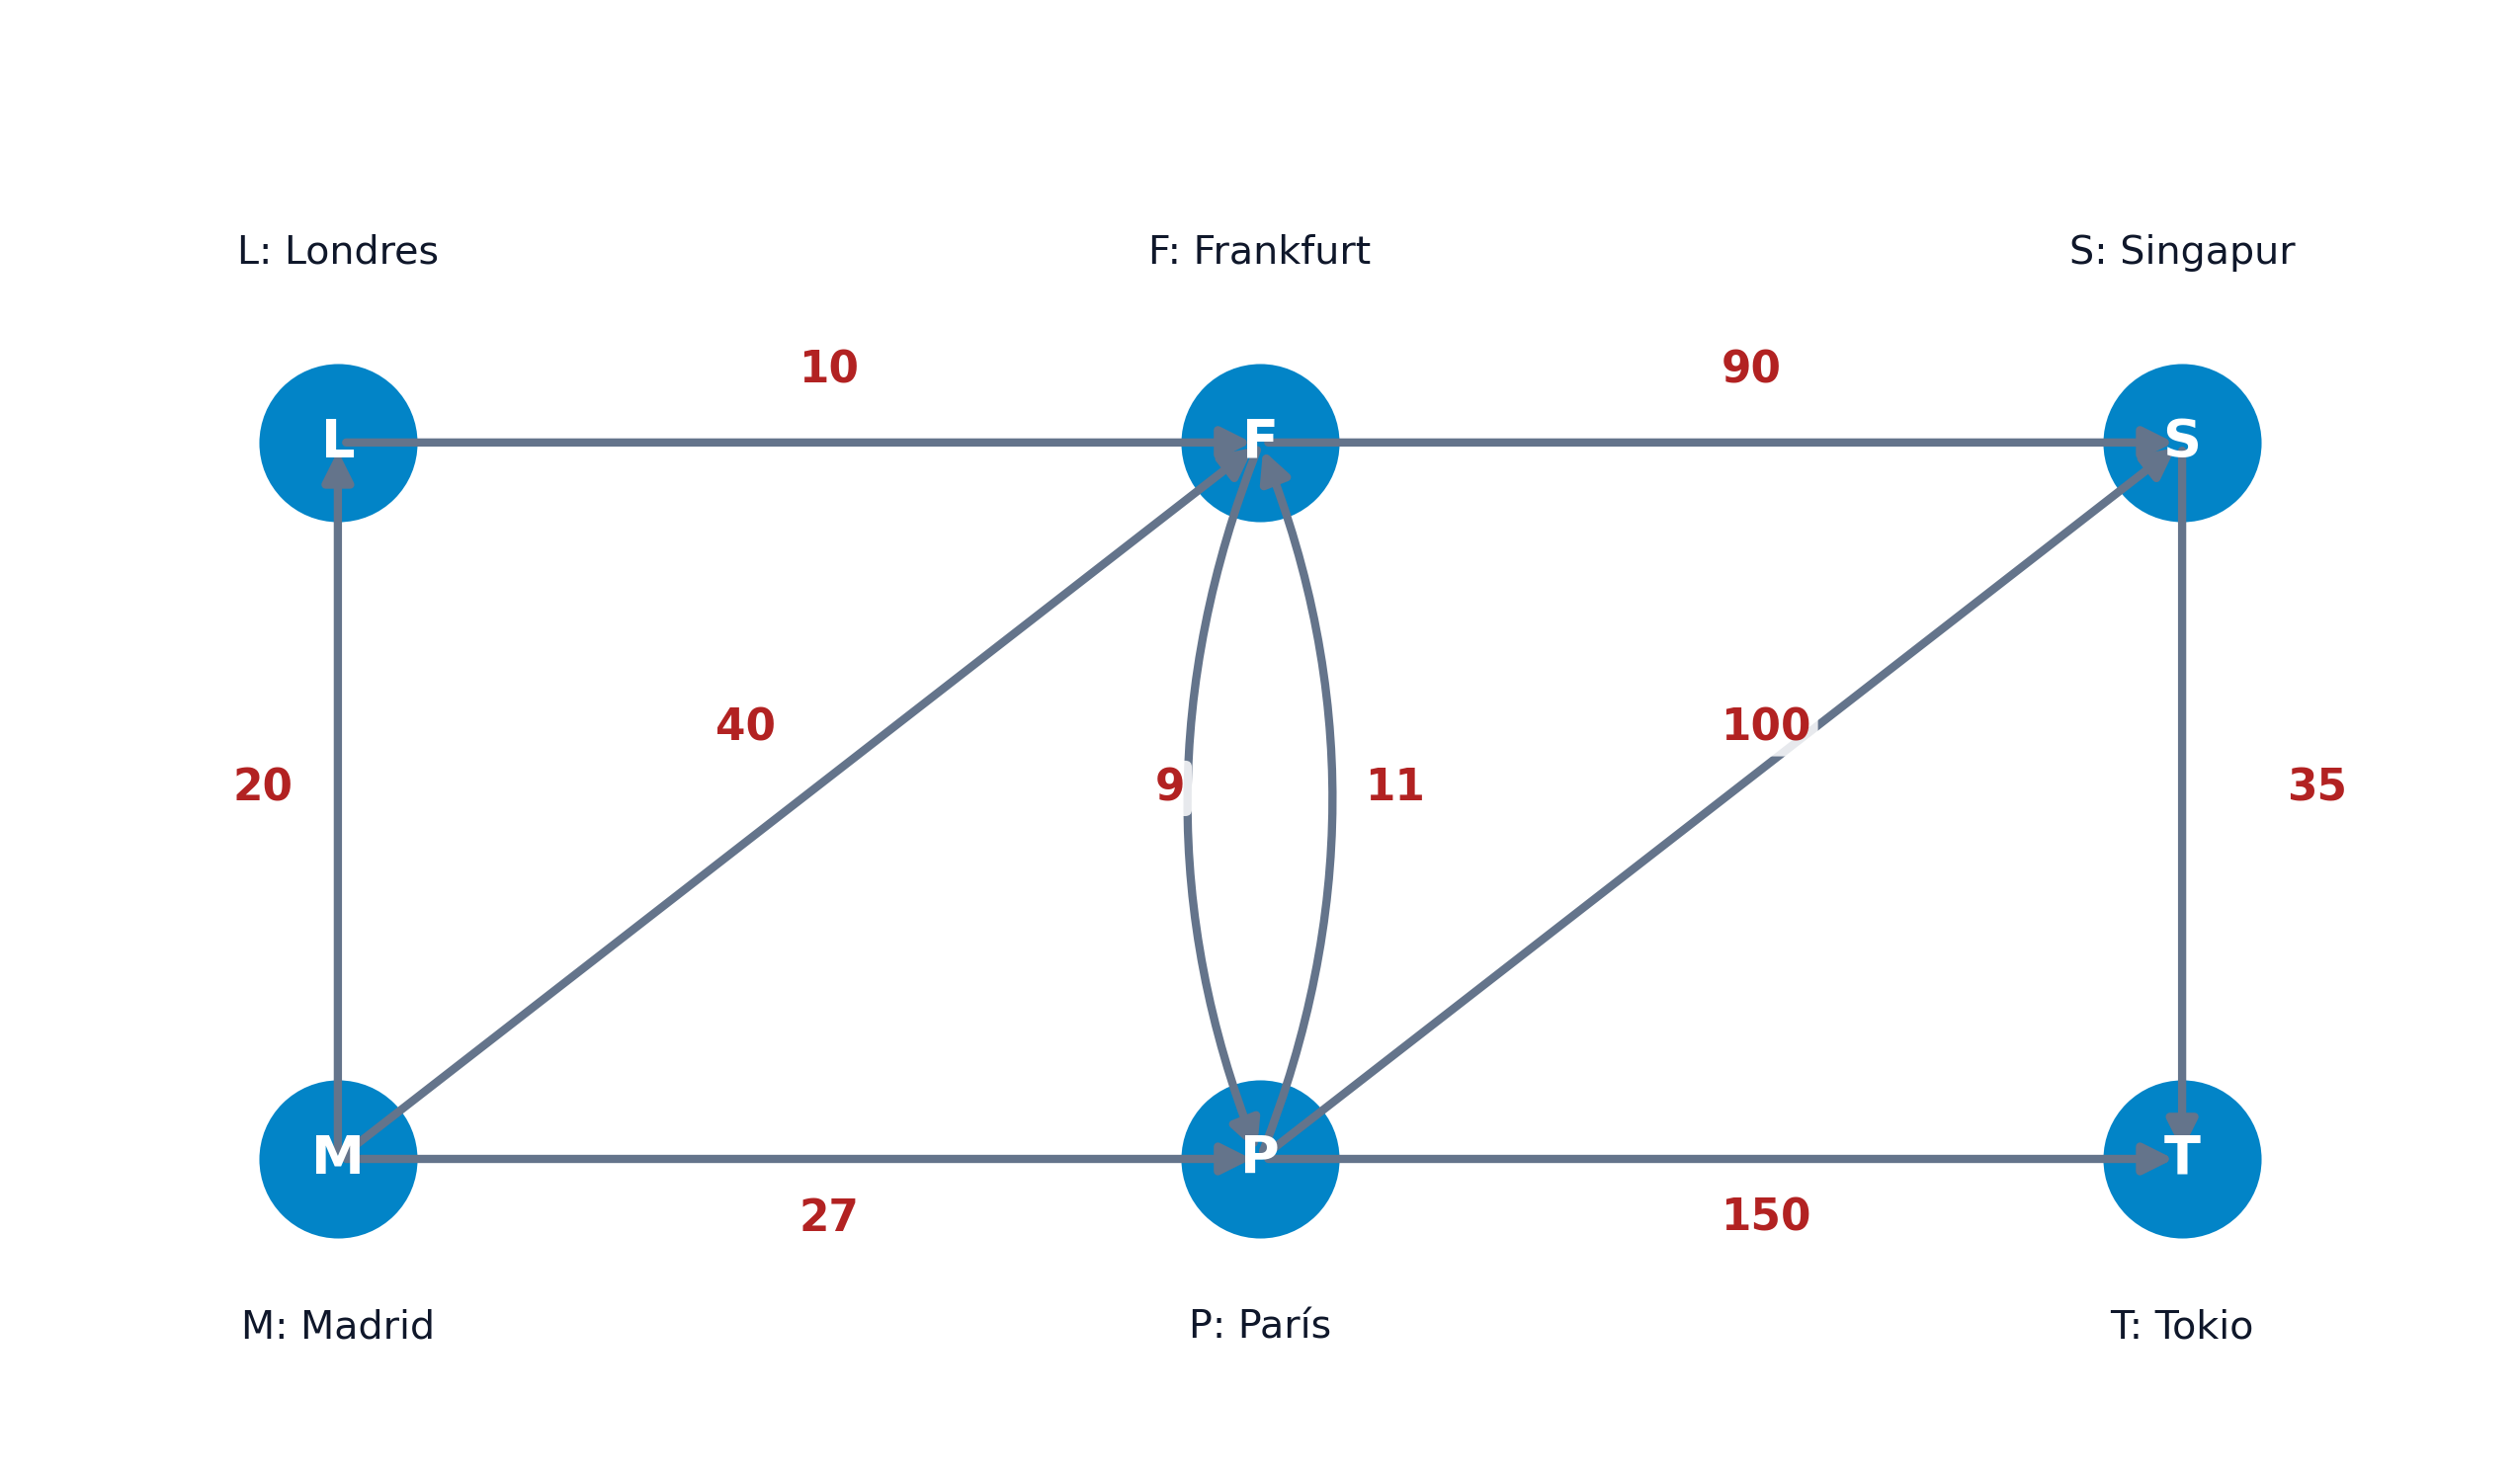
\includegraphics[width=1\linewidth,height=\textheight,keepaspectratio]{../images/cminimo_ejemplo_vuelos.png}
\end{center}
\end{column}
\end{columns}
\end{frame}

\begin{frame}{Ejemplo: Transporte marítimo con costes y beneficios}
\phantomsection\label{ejemplo-transporte-maruxedtimo-con-costes-y-beneficios}
\begin{columns}[T]
\begin{column}{0.55\linewidth}
\begin{itemize}
\tightlist
\item
  \textbf{Planteamiento}: Itinerario óptimo de navegación entre un
  puerto origen \(O\) y un puerto destino \(D\).
\item
  \textbf{Modelado dual de pesos}:

  \begin{itemize}
  \tightlist
  \item
    \textbf{Costes de combustible}: Valores positivos (\(d_{ij} > 0\)).
  \item
    \textbf{Beneficios de recarga}: Valores negativos (\(d_{ij} < 0\)).
  \end{itemize}
\item
  \textbf{Solución}: Minimizar costes en la red equivale a maximizar el
  beneficio neto total acumulado.
\end{itemize}
\end{column}

\begin{column}{0.45\linewidth}
\begin{tcolorbox}[enhanced jigsaw, arc=.35mm, title=\textcolor{quarto-callout-note-color}{\faInfo}\hspace{0.5em}{Diferencia fundamental con el MST}, titlerule=0mm, opacitybacktitle=0.6, left=2mm, rightrule=.15mm, colback=white, colframe=quarto-callout-note-color-frame, toprule=.15mm, opacityback=0, coltitle=black, breakable, colbacktitle=quarto-callout-note-color!10!white, bottomtitle=1mm, leftrule=.75mm, bottomrule=.15mm, toptitle=1mm]

A diferencia del MST (solución siempre finita), el camino mínimo con
arcos negativos puede presentar \textbf{divergencia a \(-\infty\)}.

\end{tcolorbox}
\end{column}
\end{columns}
\end{frame}

\begin{frame}{Paradoja del camino en grafos con circuitos negativos}
\phantomsection\label{paradoja-del-camino-en-grafos-con-circuitos-negativos}
\begin{columns}[T]
\begin{column}{0.5\linewidth}
\begin{itemize}
\item
  \textbf{Ruta simple inicial}: \(\mu_1 = (a, b, e, f)\) con coste:
  \[d(\mu_1) = 3 + (-6) + 2 = -1\]
\item
  \textbf{Circuito de coste negativo}: \(\mu_C = (b, e, f, b)\) con
  coste: \[d(\mu_C) = -6 + 2 + 2 = -2 < 0\]
\item
  \textbf{Divergencia a \(-\infty\)}: Dar \(k\) vueltas a \(\mu_C\)
  reduce el coste a:
  \[d(\mu_k) = -1 - 2k \xrightarrow[k \to \infty]{} -\infty\]
\end{itemize}
\end{column}

\begin{column}{0.5\linewidth}
\end{column}
\end{columns}
\end{frame}

\begin{frame}{Condición de existencia de solución óptima finita}
\phantomsection\label{condiciuxf3n-de-existencia-de-soluciuxf3n-uxf3ptima-finita}
\begin{tcolorbox}[enhanced jigsaw, arc=.35mm, title=\textcolor{quarto-callout-important-color}{\faExclamation}\hspace{0.5em}{Condición de existencia de solución óptima finita}, titlerule=0mm, opacitybacktitle=0.6, left=2mm, rightrule=.15mm, colback=white, colframe=quarto-callout-important-color-frame, toprule=.15mm, opacityback=0, coltitle=black, breakable, colbacktitle=quarto-callout-important-color!10!white, bottomtitle=1mm, leftrule=.75mm, bottomrule=.15mm, toptitle=1mm]

Dada una red dirigida \(G = (V, U, \mathbf{d})\) y dos vértices
\(s, t \in V\), existe una solución óptima finita al problema del camino
mínimo si y sólo si se cumplen:

\begin{itemize}
\item
  \textbf{Hipótesis \(H_1\) (Accesibilidad)}: Existe al menos un camino
  dirigido que conecta el nodo origen \(s\) con el destino \(t\).
\item
  \textbf{Hipótesis \(H_2\) (Ausencia de circuitos de coste negativo)}:
  Ningún camino dirigido de \(s\) a \(t\) contiene un circuito de coste
  total estrictamente negativo.
\end{itemize}

\end{tcolorbox}
\end{frame}

\section{Ecuaciones de optimalidad de
Bellman}\label{ecuaciones-de-optimalidad-de-bellman}

\begin{frame}{Principio de Optimalidad de Bellman (1957)}
\phantomsection\label{principio-de-optimalidad-de-bellman-1957}
\begin{tcolorbox}[enhanced jigsaw, arc=.35mm, title=\textcolor{quarto-callout-note-color}{\faInfo}\hspace{0.5em}{Principio de Optimalidad de Bellman}, titlerule=0mm, opacitybacktitle=0.6, left=2mm, rightrule=.15mm, colback=white, colframe=quarto-callout-note-color-frame, toprule=.15mm, opacityback=0, coltitle=black, breakable, colbacktitle=quarto-callout-note-color!10!white, bottomtitle=1mm, leftrule=.75mm, bottomrule=.15mm, toptitle=1mm]

Una secuencia óptima de decisiones que resuelve un problema de
optimización multietapa debe cumplir la propiedad de que, cualquiera que
sea el estado inicial y la decisión inicial adoptada, las decisiones
restantes deben constituir una \textbf{política óptima} respecto al
estado resultante.

\emph{(Toda subpolítica de una política óptima es a su vez una
subpolítica óptima)}

\end{tcolorbox}

\begin{itemize}
\tightlist
\item
  \textbf{Interpretación en caminos mínimos}: Si el camino mínimo entre
  \(s\) y \(t\) es \(\mu^*[s, t]\) y pasa por los vértices intermedios
  \(i\) y \(j\), la subruta \(\mu^*[i, j]\) es obligatoriamente el
  camino mínimo entre \(i\) y \(j\).
\end{itemize}
\end{frame}

\begin{frame}{Ecuaciones de optimalidad de Bellman}
\phantomsection\label{ecuaciones-de-optimalidad-de-bellman-1}
\begin{tcolorbox}[enhanced jigsaw, arc=.35mm, title=\textcolor{quarto-callout-important-color}{\faExclamation}\hspace{0.5em}{Ecuaciones de optimalidad de Bellman}, titlerule=0mm, opacitybacktitle=0.6, left=2mm, rightrule=.15mm, colback=white, colframe=quarto-callout-important-color-frame, toprule=.15mm, opacityback=0, coltitle=black, breakable, colbacktitle=quarto-callout-important-color!10!white, bottomtitle=1mm, leftrule=.75mm, bottomrule=.15mm, toptitle=1mm]

En una red dirigida sin circuitos de coste negativo, las distancias
mínimas \(u_j\) desde el origen \(s = 1\) a los vértices
\(j = 2, \dots, n\) satisfacen:

\[
\begin{aligned}
u_1 &= 0 \\
u_j &= \min_{k \neq j} \{ u_k + d_{kj} \}, \quad \forall j = 2, \dots, n
\end{aligned}
\]

\end{tcolorbox}

\begin{itemize}
\tightlist
\item
  Físicamente expresan que la distancia a \(j\) es el mínimo entre las
  distancias acumuladas a sus predecesores \(k\) más el coste del arco
  directo \((k, j)\).
\end{itemize}
\end{frame}

\begin{frame}{Ejemplo: Planteamiento de las ecuaciones de Bellman}
\phantomsection\label{ejemplo-planteamiento-de-las-ecuaciones-de-bellman}
\begin{columns}[T]
\begin{column}{0.5\linewidth}
\begin{center}
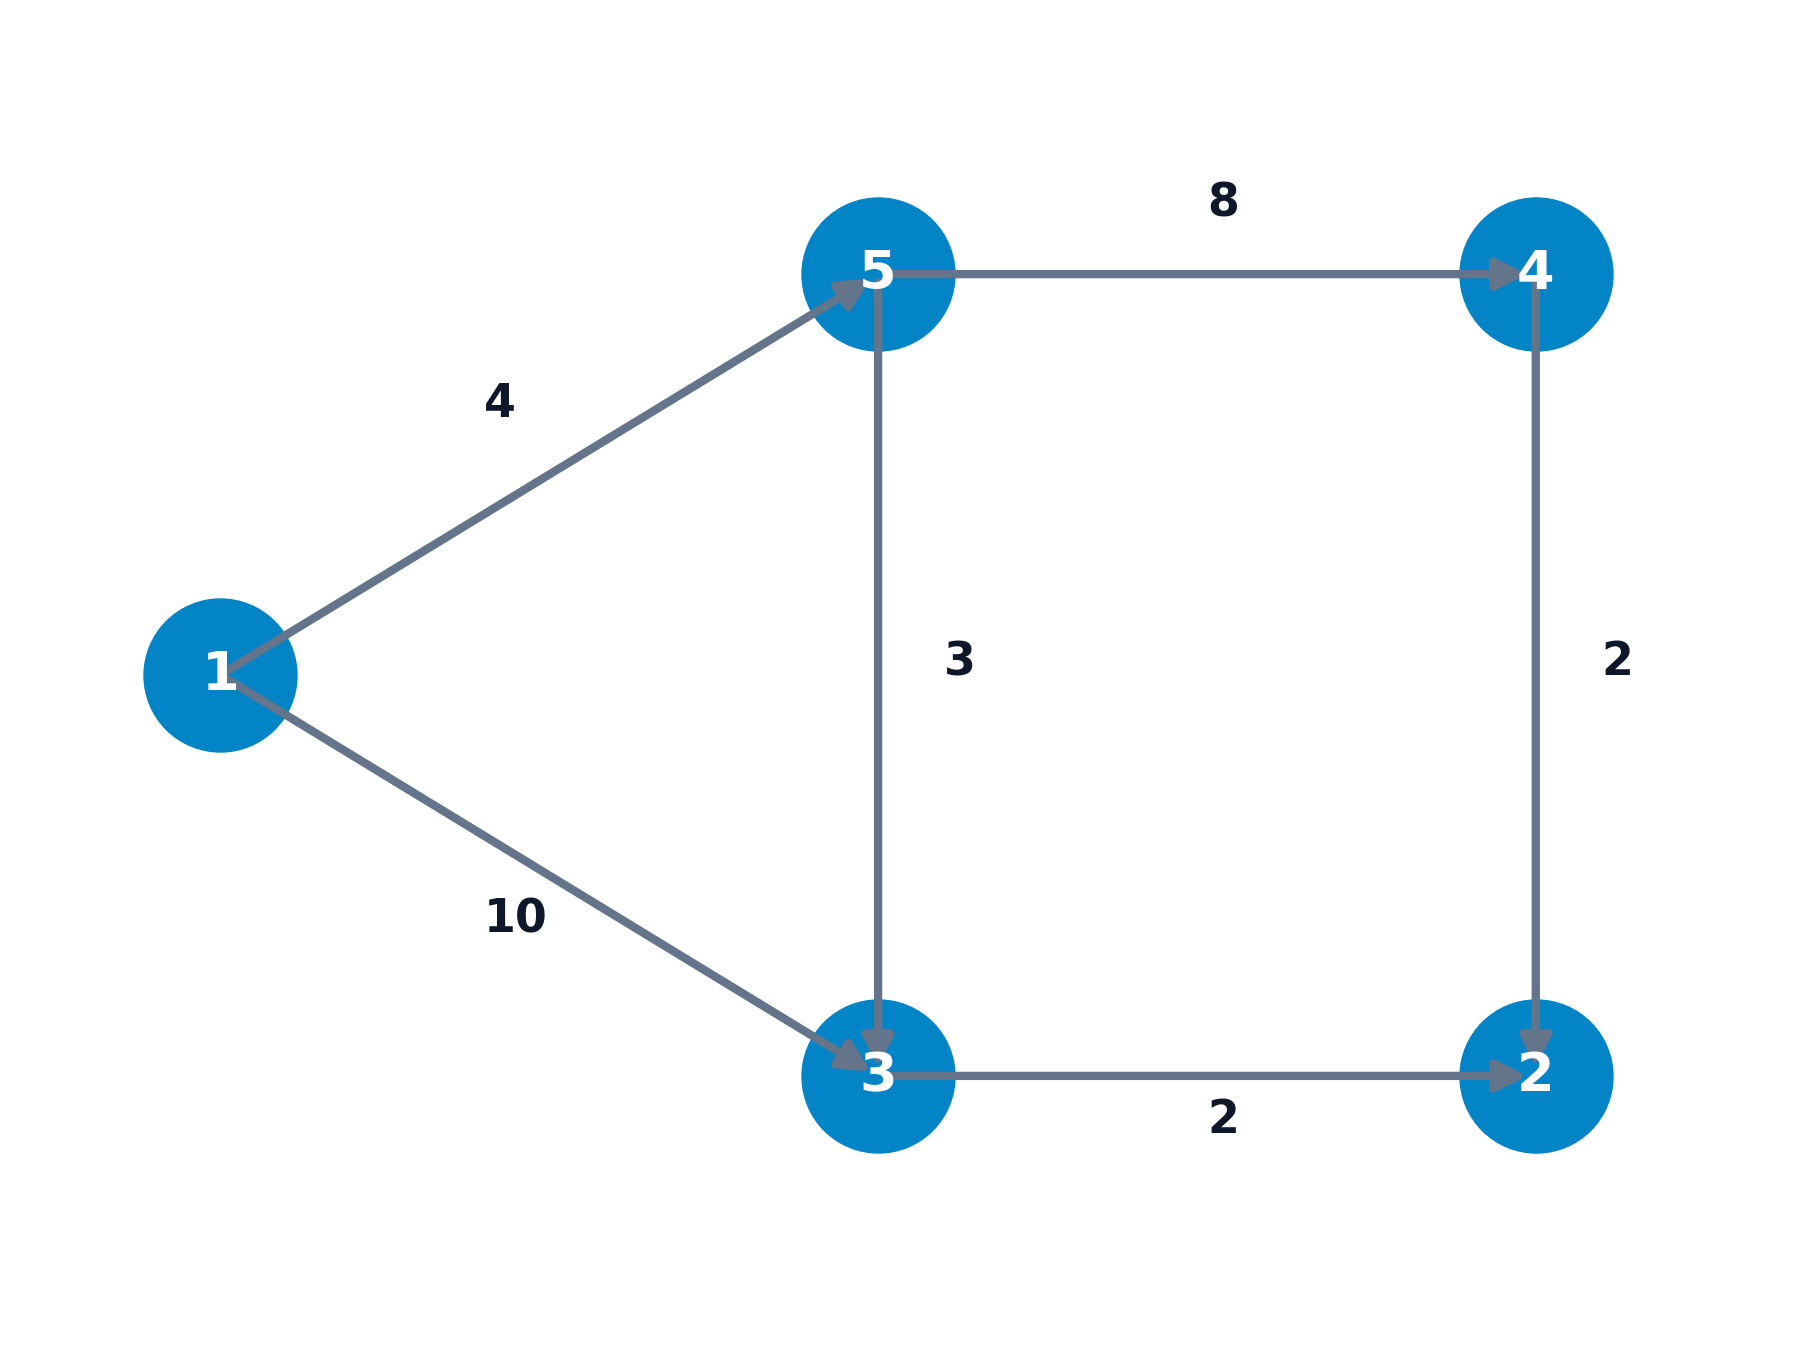
\includegraphics[width=0.95\linewidth,height=\textheight,keepaspectratio]{../images/bellman_ecuaciones_ejemplo.png}
\end{center}
\end{column}

\begin{column}{0.5\linewidth}
\begin{itemize}
\item
  \textbf{Formulación del sistema para \(s = 1\)}: \[
  \begin{aligned}
  u_1 &= 0 \\
  u_5 &= \min \{ u_1 + 4 \} = 4 \\
  u_3 &= \min \{ u_1 + 10, u_5 + 3 \} = \min \{ 10, 7 \} = 7 \\
  u_4 &= \min \{ u_5 + 8 \} = 12 \\
  u_2 &= \min \{ u_3 + 2, u_4 + 2 \} = \min \{ 9, 14 \} = 9
  \end{aligned}
  \]
\item
  \textbf{Resultados}:

  \begin{itemize}
  \tightlist
  \item
    \(\mathbf{u} = (0, 9, 7, 12, 4)\).
  \item
    \(\text{Pred} = (1, 3, 5, 5, 1)\).
  \item
    Arborescencia: \(\{ (1,5), (5,3), (5,4), (3,2) \}\).
  \end{itemize}
\end{itemize}
\end{column}
\end{columns}
\end{frame}

\begin{frame}{Insuficiencia y no unicidad ante circuitos de coste nulo}
\phantomsection\label{insuficiencia-y-no-unicidad-ante-circuitos-de-coste-nulo}
\begin{columns}[T]
\begin{column}{0.45\linewidth}
\begin{center}
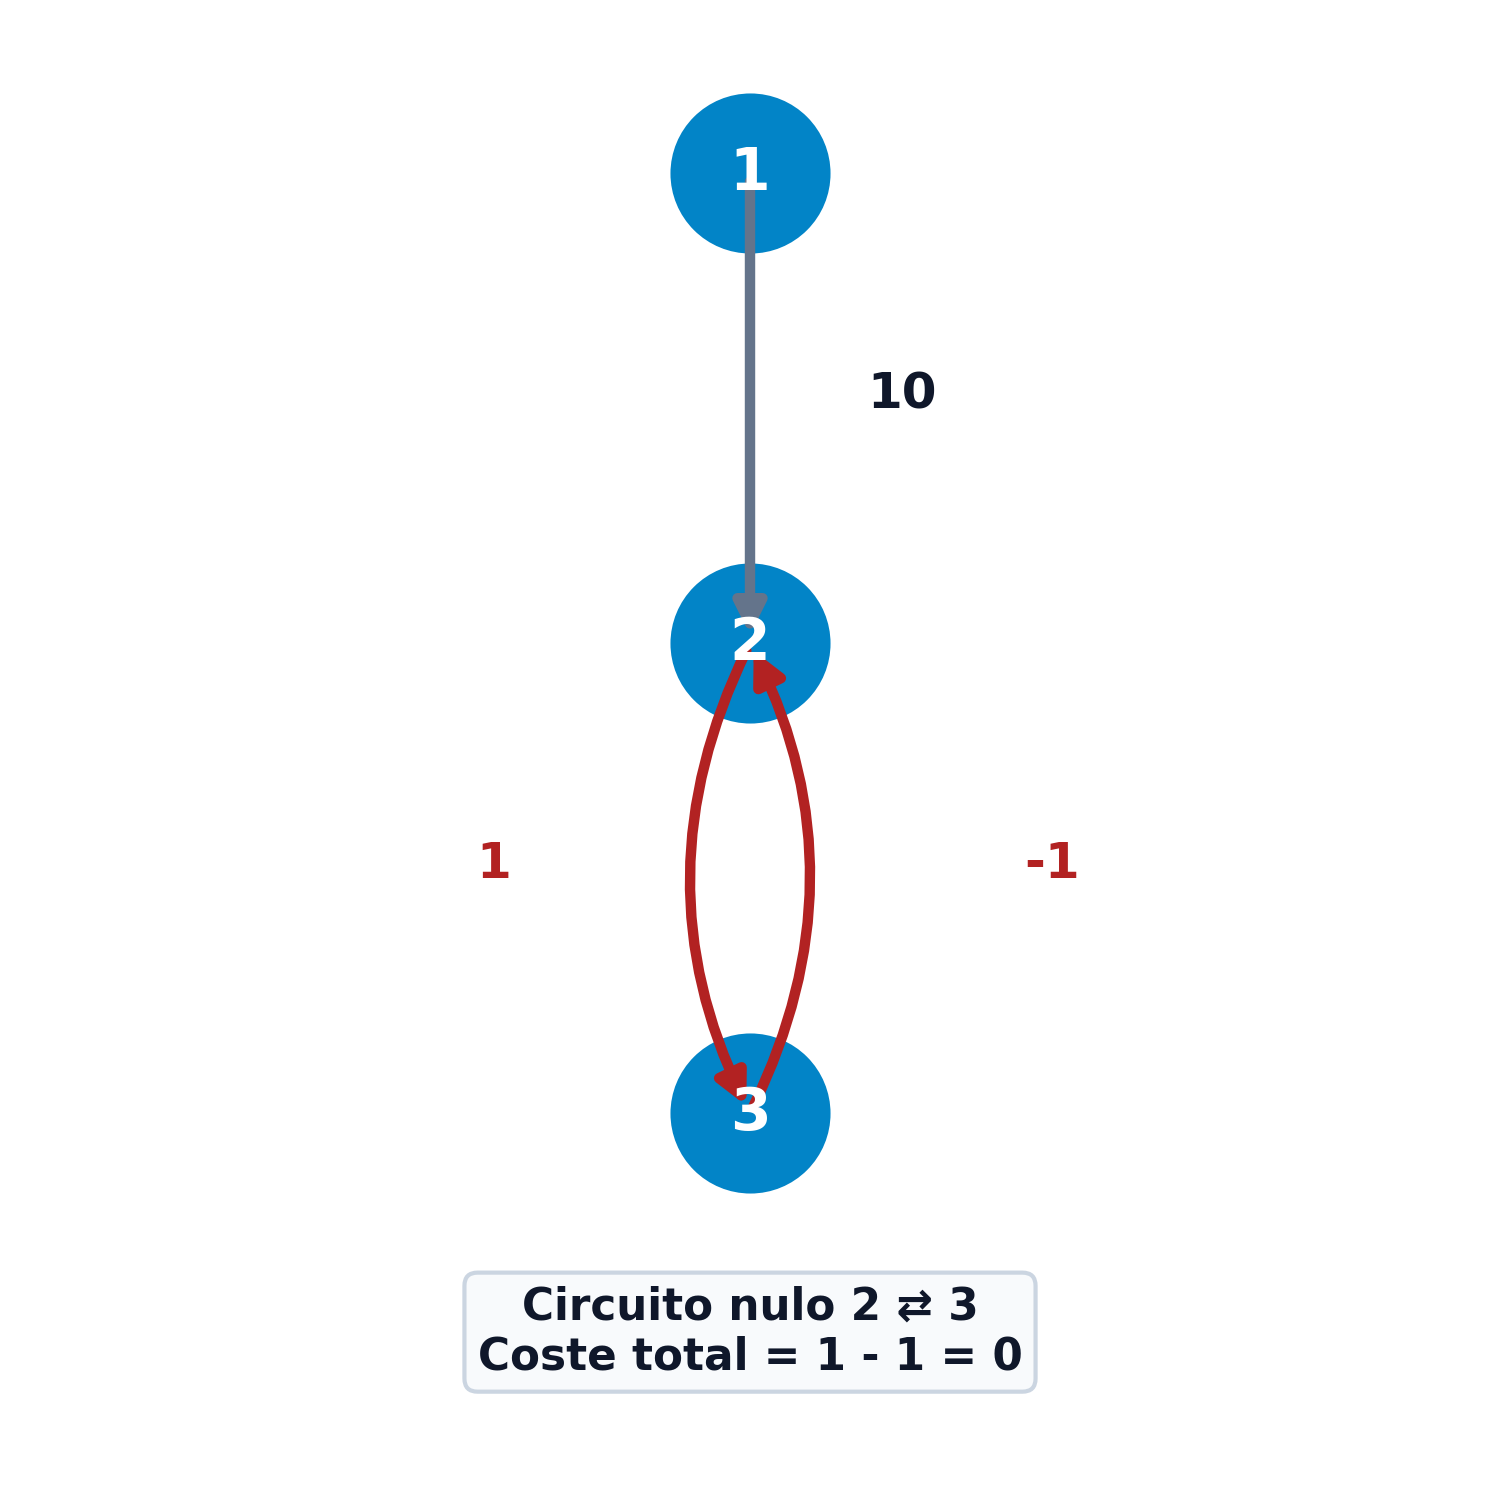
\includegraphics[width=0.95\linewidth,height=\textheight,keepaspectratio]{../images/cminimo_circuito_nulo.png}
\end{center}
\end{column}

\begin{column}{0.55\linewidth}
\begin{itemize}
\item
  \textbf{Circuito de coste nulo}: \(2 \rightleftarrows 3\) con
  \(d_{23} + d_{32} = 1 + (-1) = 0\).
\item
  \textbf{Sistema de ecuaciones de Bellman}: \[
  \begin{aligned}
  u_1 &= 0 \\
  u_2 &= \min \{ 10, u_3 - 1 \} \\
  u_3 &= u_2 + 1
  \end{aligned}
  \]
\item
  \textbf{Múltiples soluciones algebraicas}:

  \begin{itemize}
  \tightlist
  \item
    \(\mathbf{u} = (0, 10, 11) \implies\) \textbf{Solución física real}.
  \item
    \(\mathbf{u} = (0, 5, 6) \implies\) Satisface las ecuaciones pero
    \textbf{es falsa}.
  \end{itemize}
\end{itemize}
\end{column}
\end{columns}
\end{frame}

\begin{frame}{Proposición: Arborescencia asociada a Bellman}
\phantomsection\label{proposiciuxf3n-arborescencia-asociada-a-bellman}
\begin{tcolorbox}[enhanced jigsaw, arc=.35mm, title=\textcolor{quarto-callout-note-color}{\faInfo}\hspace{0.5em}{Construcción de la arborescencia soporte}, titlerule=0mm, opacitybacktitle=0.6, left=2mm, rightrule=.15mm, colback=white, colframe=quarto-callout-note-color-frame, toprule=.15mm, opacityback=0, coltitle=black, breakable, colbacktitle=quarto-callout-note-color!10!white, bottomtitle=1mm, leftrule=.75mm, bottomrule=.15mm, toptitle=1mm]

Las ecuaciones de optimalidad de Bellman:

\[
u_1 = 0, \quad u_j = \min_{k \neq j} \{ u_k + d_{kj} \}, \quad \forall j \neq 1
\]

permiten construir de forma \textbf{única} la arborescencia de caminos
mínimos con raíz en \(1\) si y sólo si en la red \textbf{no existen
circuitos dirigidos de coste nulo ni negativo}.

\end{tcolorbox}
\end{frame}

\begin{frame}{Ejemplo: Ecuaciones de Bellman en la red de aeropuertos}
\phantomsection\label{ejemplo-ecuaciones-de-bellman-en-la-red-de-aeropuertos}
\begin{columns}[T]
\begin{column}{0.35\linewidth}
\begin{center}
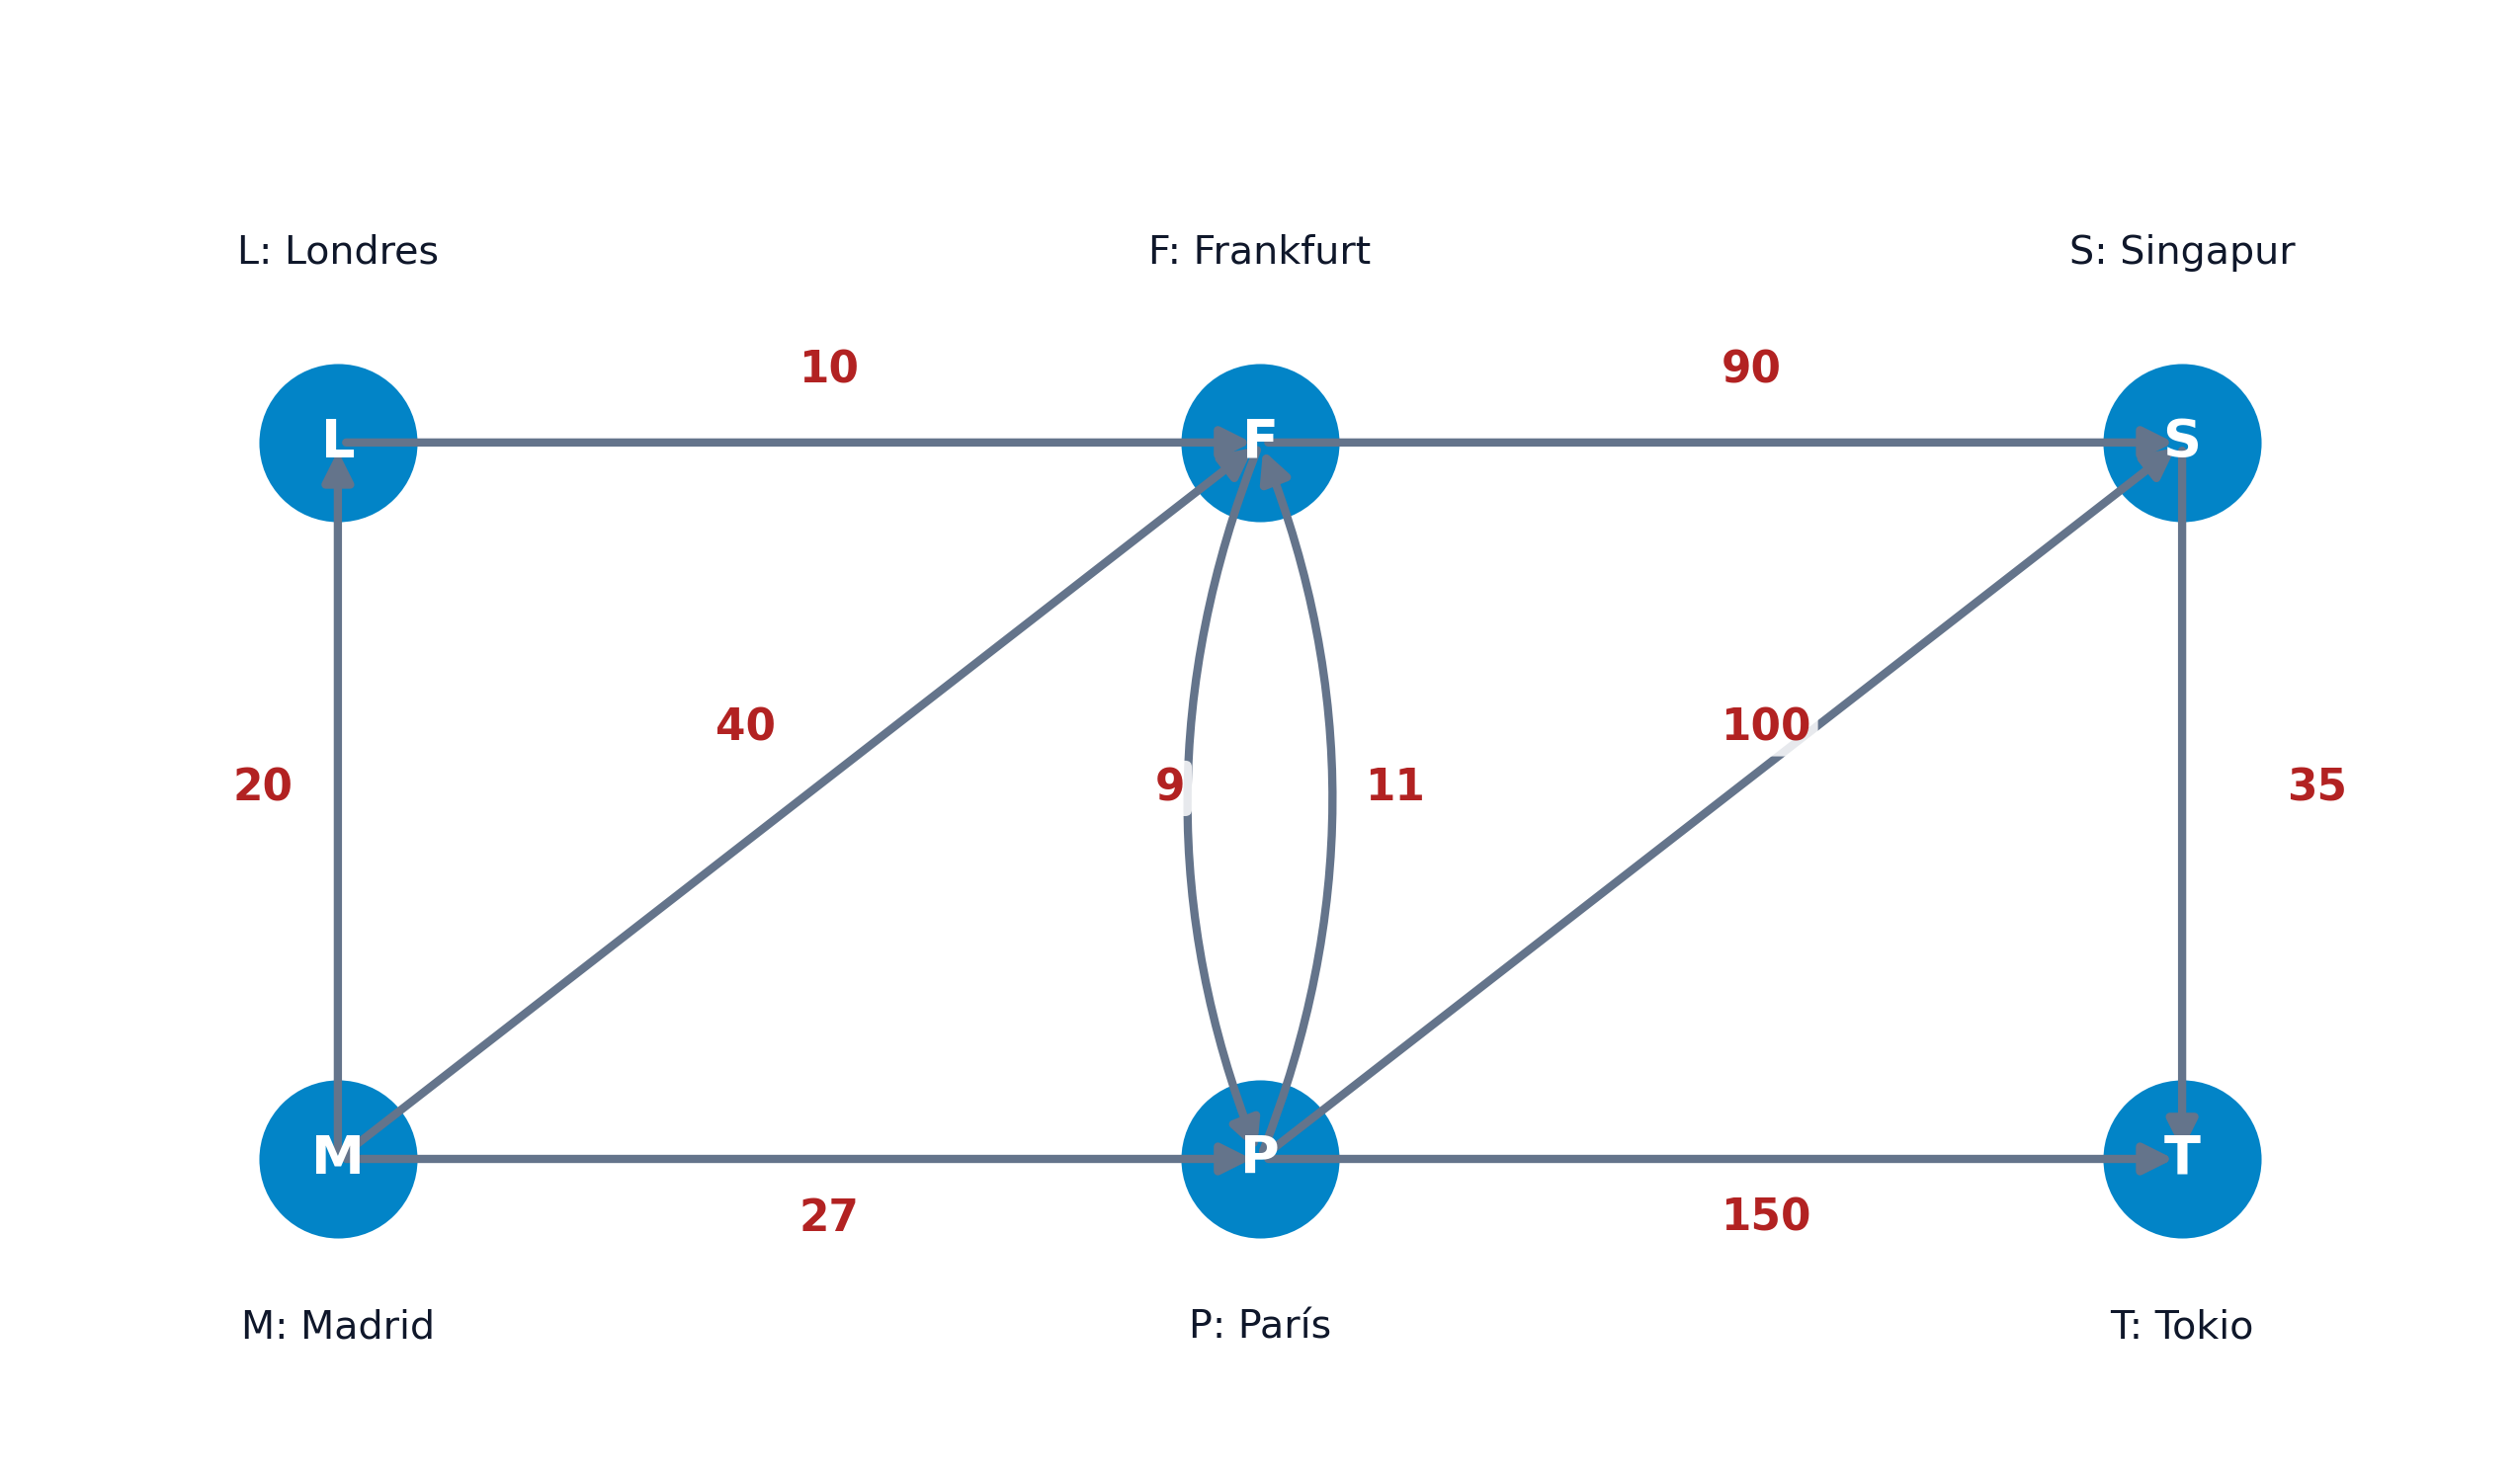
\includegraphics[width=0.95\linewidth,height=\textheight,keepaspectratio]{../images/cminimo_ejemplo_vuelos.png}
\end{center}
\end{column}

\begin{column}{0.65\linewidth}
\begin{itemize}
\item
  \textbf{Ecuaciones desde Madrid (\(M\)) - Nodos iniciales}:

  \begin{itemize}
  \tightlist
  \item
    \textbf{Madrid (\(M\))}: \(u_M = 0\)
  \item
    \textbf{Londres (\(L\))}:
    \[ \small u_L = \min \{ u_M + 20 \} = 20 \]
  \item
    \textbf{París (\(P\))}:
    \[ \small u_P = \min \{ u_M + 27, \, u_F + 9 \} = \min \{ 27, 39 \} = 27 \]
  \item
    \textbf{Frankfurt (\(F\))}: \[ \small
    \begin{aligned}
    u_F &= \min \{ u_M + 40, \, u_L + 10, \, u_P + 11 \} \\
        &= \min \{ 40, 30, 38 \} = 30
    \end{aligned}
    \]
  \end{itemize}
\end{itemize}
\end{column}
\end{columns}
\end{frame}

\begin{frame}{Ejemplo: Ecuaciones de Bellman en la red de aeropuertos
(cont.)}
\phantomsection\label{ejemplo-ecuaciones-de-bellman-en-la-red-de-aeropuertos-cont.}
\begin{columns}[T]
\begin{column}{0.35\linewidth}
\begin{center}
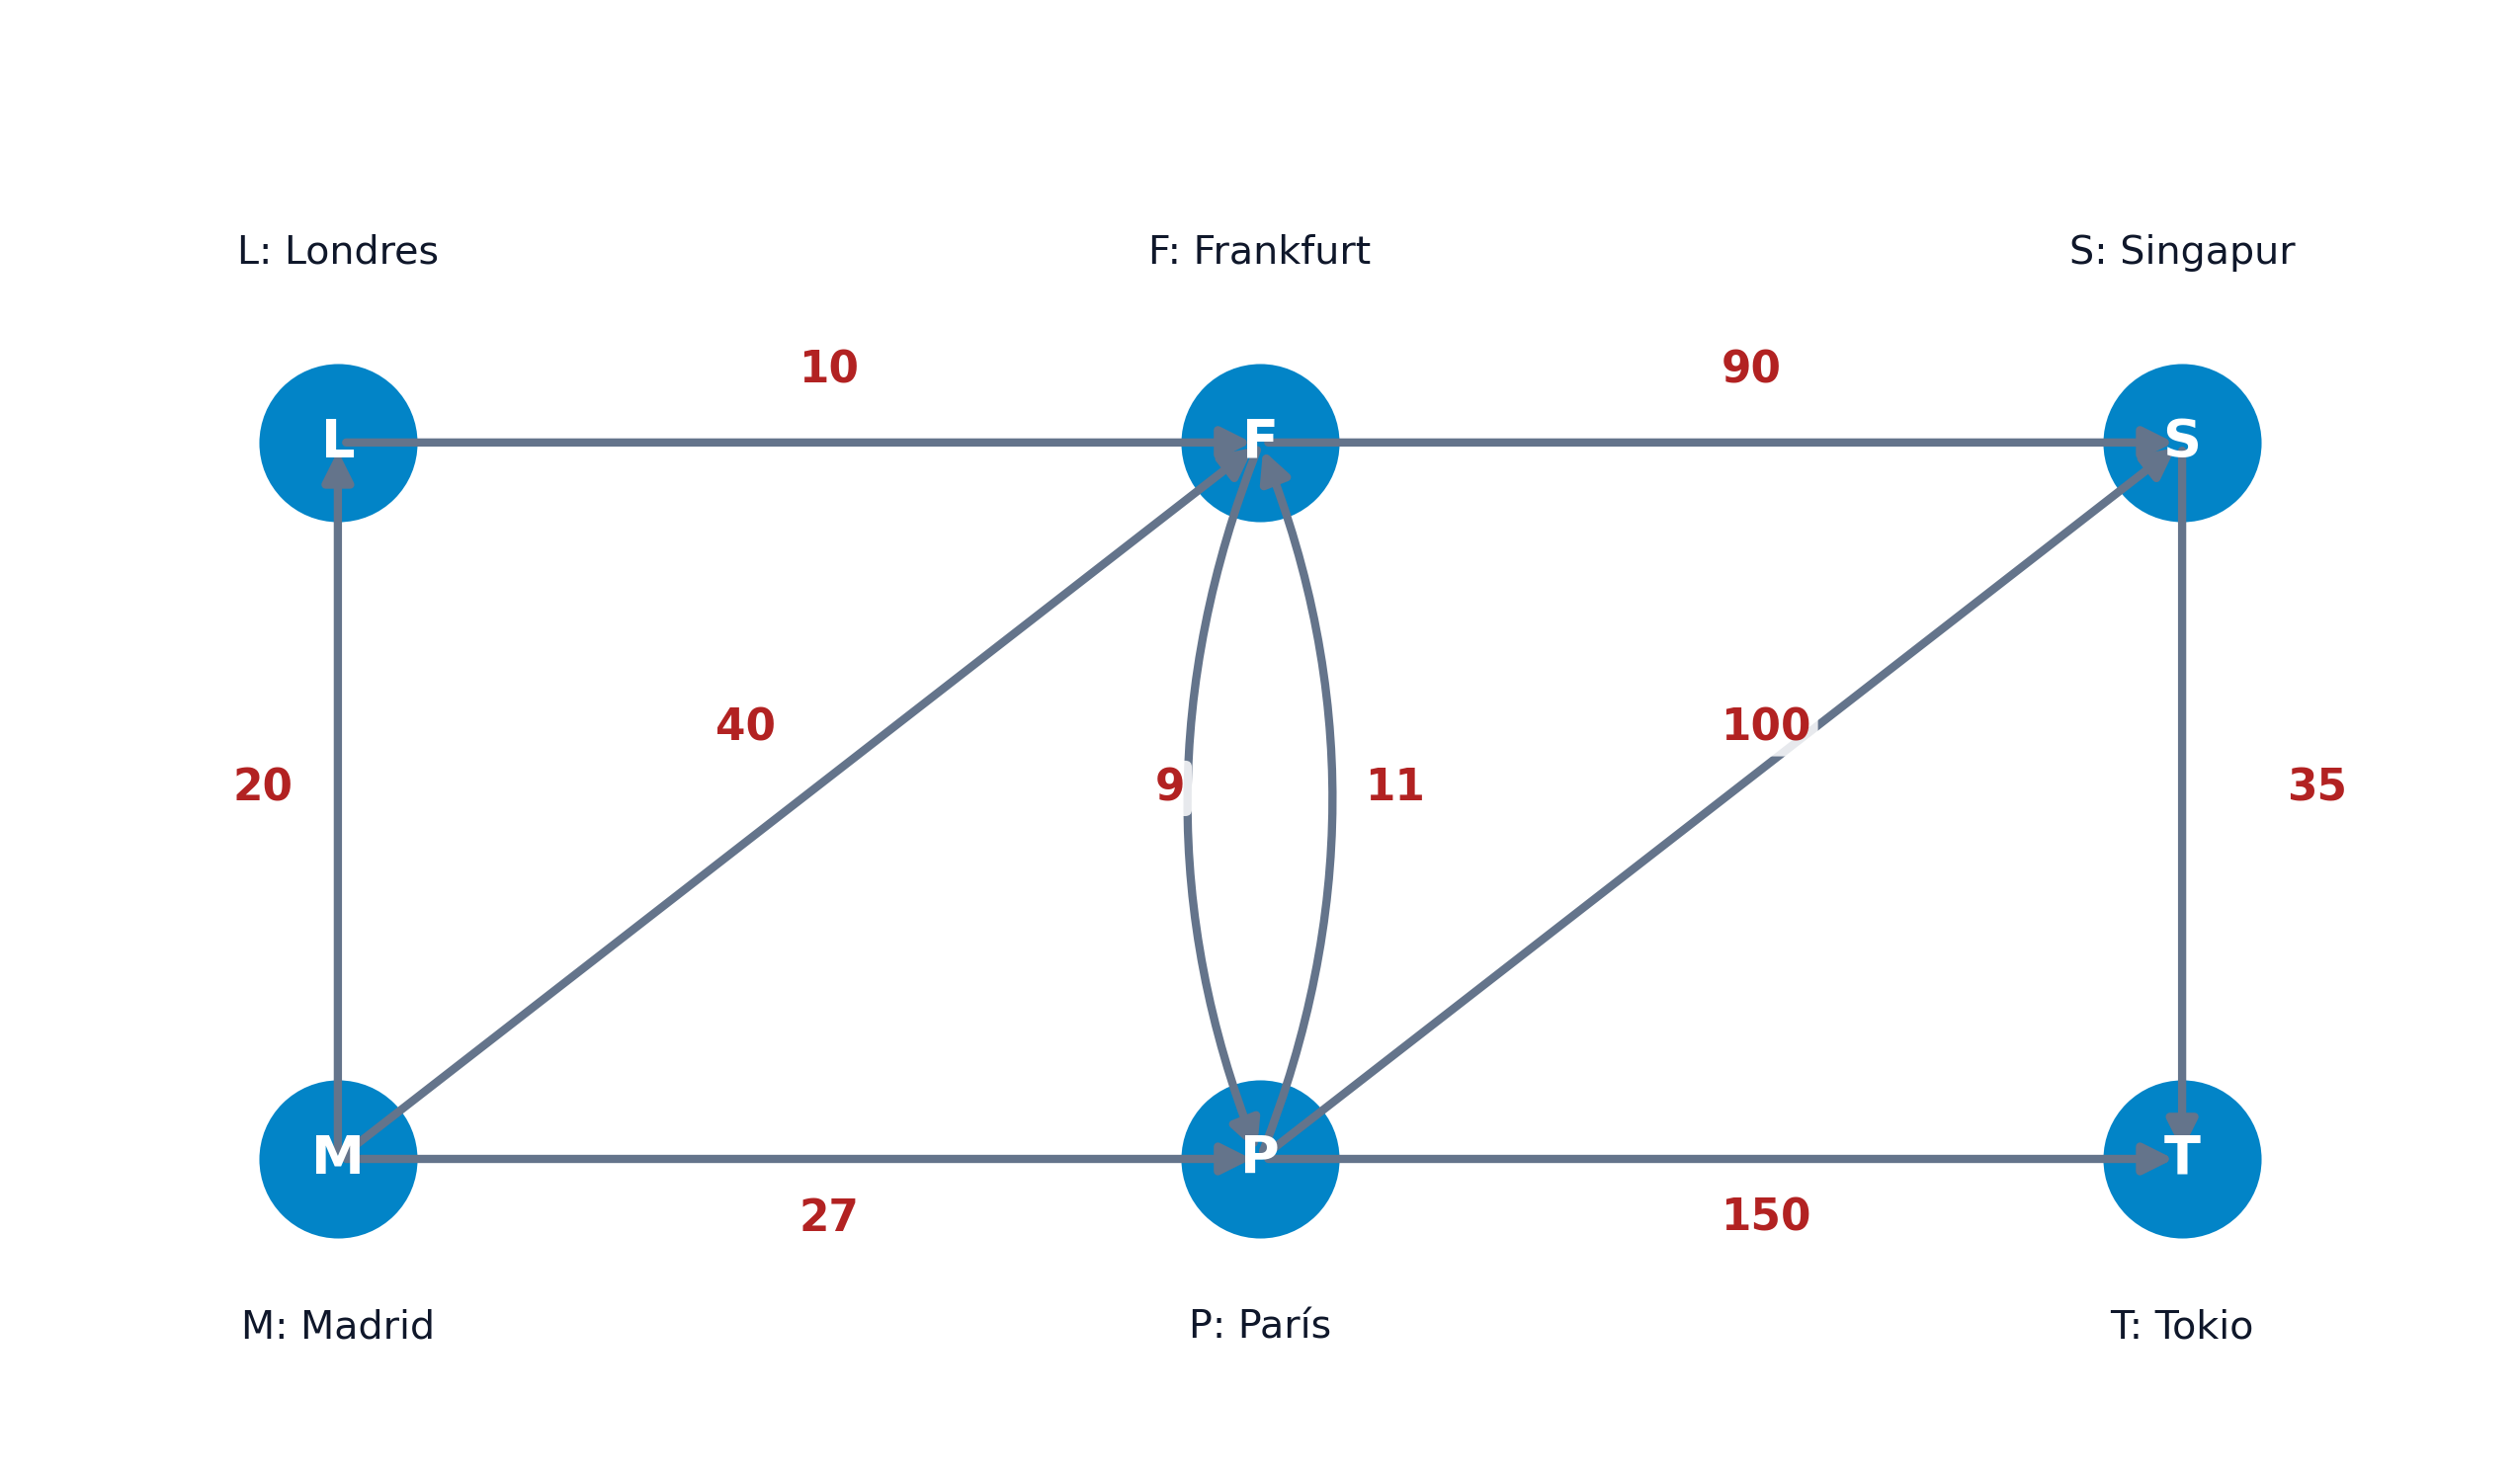
\includegraphics[width=0.95\linewidth,height=\textheight,keepaspectratio]{../images/cminimo_ejemplo_vuelos.png}
\end{center}
\end{column}

\begin{column}{0.65\linewidth}
\begin{itemize}
\item
  \textbf{Ecuaciones hacia el destino final}: \[ \small
  \begin{aligned}
  u_S &= \min \{ u_F + 90, \, u_P + 100 \} = \min \{ 120, 127 \} = 120 \\
  u_T &= \min \{ u_P + 150, \, u_S + 35 \} = \min \{ 177, 155 \} = 155
  \end{aligned}
  \]
\item
  \textbf{Solución y Arborescencia Óptima \(T^*\)}:

  \begin{itemize}
  \tightlist
  \item
    \textbf{Ruta a Tokio}: \(M \to L \to F \to S \to T\) (155 €).
  \item
    \textbf{Predecesores}:
    \(L \gets M, \, P \gets M, \, F \gets L, \, S \gets F, \, T \gets S\).
  \item
    \textbf{Arcos de \(T^*\)}:
    \(\{(M,L), (M,P), (L,F), (F,S), (S,T)\}\).
  \end{itemize}
\end{itemize}
\end{column}
\end{columns}
\end{frame}

\begin{frame}{Complejidad computacional de las ecuaciones de Bellman}
\phantomsection\label{complejidad-computacional-de-las-ecuaciones-de-bellman}
\begin{itemize}
\item
  \textbf{Complejidad factorial \(O(n!)\) en redes generales}: Sin
  conocer el orden secuencial de resolución de los vértices, explorar
  las combinaciones de predecesores requiere \(O(n!)\) comparaciones.
\item
  \textbf{Reducción de complejidad mediante ordenación topológica}: Si
  los nodos se ordenan secuencialmente de forma adecuada, la complejidad
  se reduce a \textbf{\(O(n^2)\)} o tiempo estrictamente \textbf{lineal
  \(O(|V| + |U|)\)}.
\item
  \textbf{Condición necesaria}: La ordenación topológica secuencial
  exige que el digrafo \textbf{no contenga circuitos dirigidos} (DAGs).
\end{itemize}
\end{frame}

\section{Redes sin circuitos (DAGs) y ordenación
topológica}\label{redes-sin-circuitos-dags-y-ordenaciuxf3n-topoluxf3gica}

\begin{frame}{Caracterización de digrafos acíclicos (DAGs)}
\phantomsection\label{caracterizaciuxf3n-de-digrafos-acuxedclicos-dags}
\begin{tcolorbox}[enhanced jigsaw, arc=.35mm, title=\textcolor{quarto-callout-note-color}{\faInfo}\hspace{0.5em}{Caracterización mediante ordenación topológica}, titlerule=0mm, opacitybacktitle=0.6, left=2mm, rightrule=.15mm, colback=white, colframe=quarto-callout-note-color-frame, toprule=.15mm, opacityback=0, coltitle=black, breakable, colbacktitle=quarto-callout-note-color!10!white, bottomtitle=1mm, leftrule=.75mm, bottomrule=.15mm, toptitle=1mm]

Un digrafo \(G = (V, U)\) no tiene circuitos dirigidos si y sólo si
existe una numeración de sus \(n\) vértices \(v_1, v_2, \dots, v_n\) tal
que para todo arco dirigidos \((i, j) \in U\) se cumple:

\[i < j\]

\end{tcolorbox}

\begin{itemize}
\tightlist
\item
  \textbf{Consecuencia matemática}: Todos los arcos de la red avanzan
  estrictamente de izquierda a derecha. No existen arcos de retroceso
  que puedan formar bucles.
\end{itemize}
\end{frame}

\begin{frame}{Ejemplo: Verificación de ordenación topológica}
\phantomsection\label{ejemplo-verificaciuxf3n-de-ordenaciuxf3n-topoluxf3gica}
\begin{columns}[T]
\begin{column}{0.5\linewidth}
\begin{center}
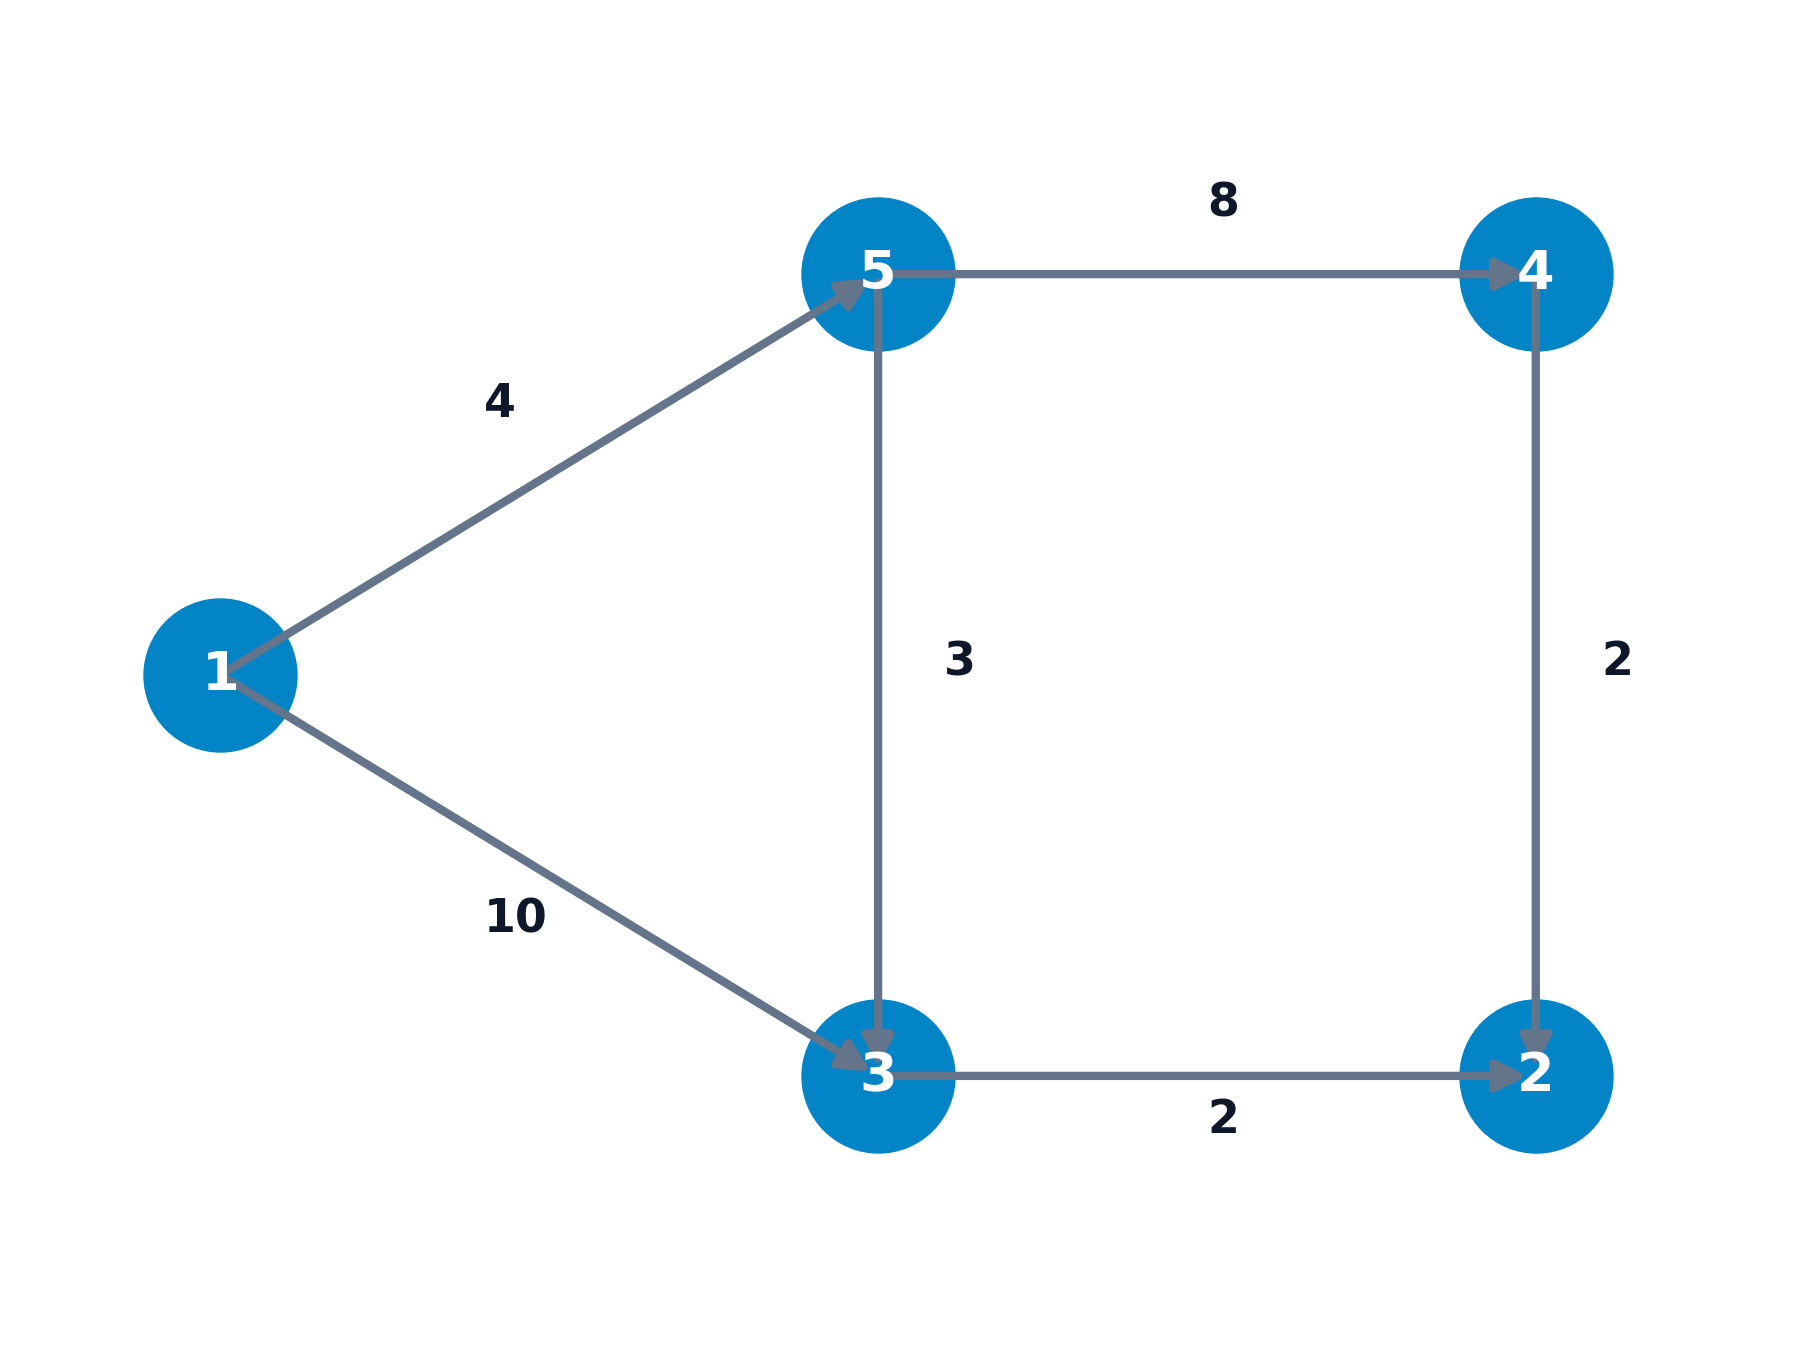
\includegraphics[width=0.9\linewidth,height=\textheight,keepaspectratio]{../images/bellman_ecuaciones_ejemplo.png}
\end{center}
\end{column}

\begin{column}{0.5\linewidth}
\begin{itemize}
\item
  \textbf{Secuencia propuesta}: \((1, 5, 3, 4, 2)\)
\item
  \textbf{Chequeo de arcos}:

  \begin{itemize}
  \tightlist
  \item
    \((1, 5) \implies 1^\circ \to 2^\circ\) (cumple \(i < j\))
  \item
    \((1, 3) \implies 1^\circ \to 3^\circ\) (cumple \(i < j\))
  \item
    \((5, 4) \implies 2^\circ \to 4^\circ\) (cumple \(i < j\))
  \item
    \((5, 3) \implies 2^\circ \to 3^\circ\) (cumple \(i < j\))
  \item
    \((4, 2) \implies 4^\circ \to 5^\circ\) (cumple \(i < j\))
  \item
    \((3, 2) \implies 3^\circ \to 5^\circ\) (cumple \(i < j\))
  \end{itemize}
\end{itemize}
\end{column}
\end{columns}
\end{frame}

\begin{frame}{Esquema del algoritmo de ordenación topológica}
\phantomsection\label{esquema-del-algoritmo-de-ordenaciuxf3n-topoluxf3gica}
\begin{tcolorbox}[enhanced jigsaw, arc=.35mm, title=\textcolor{quarto-callout-note-color}{\faInfo}\hspace{0.5em}{Algoritmo de numeración topológica}, titlerule=0mm, opacitybacktitle=0.6, left=2mm, rightrule=.15mm, colback=white, colframe=quarto-callout-note-color-frame, toprule=.15mm, opacityback=0, coltitle=black, breakable, colbacktitle=quarto-callout-note-color!10!white, bottomtitle=1mm, leftrule=.75mm, bottomrule=.15mm, toptitle=1mm]

Dada la red dirigida \(G = (V, U)\) con \(n = |V|\) vértices:

\begin{enumerate}
\tightlist
\item
  \textbf{Paso 0}: Hacer \(k \leftarrow 1\), \(V' \leftarrow V\),
  \(U' \leftarrow U\).
\item
  \textbf{Paso 1}: Seleccionar un nodo fuente \(i \in V'\) con grado de
  entrada \(d^-(i) = 0\) en \(U'\).
\item
  \textbf{Paso 2}: Asignar al nodo \(i\) el orden \(k\). Eliminar \(i\)
  y sus arcos incidentes:
  \[V' \leftarrow V' \setminus \{i\}, \quad U' \leftarrow U' \setminus \{ (i, j) \}\]
\item
  \textbf{Paso 3}: Si \(k = n\), \textbf{parar}. En otro caso, hacer
  \(k \leftarrow k + 1\) y regresar al Paso 1.
\end{enumerate}

\end{tcolorbox}
\end{frame}

\begin{frame}{Resolución de Bellman en tiempo lineal en DAGs}
\phantomsection\label{resoluciuxf3n-de-bellman-en-tiempo-lineal-en-dags}
\begin{itemize}
\item
  \textbf{Fórmula de recurrencia en orden topológico}: \[
  \begin{aligned}
  u_1 &= 0 \\
  u_j &= \min_{i < j, \, (i, j) \in U} \{ u_i + d_{ij} \}, \quad \forall j = 2, \dots, n
  \end{aligned}
  \]
\item
  \textbf{Complejidad algorítmica}: Cada arco de la red se examina
  exactamente una vez durante el recorrido secuencial.
  \[\text{Tiempo total} = O(|V| + |U|)\]
\end{itemize}
\end{frame}

\begin{frame}{Ejemplo DAG: Grafo acíclico de 7 nodos}
\phantomsection\label{ejemplo-dag-grafo-acuxedclico-de-7-nodos}
\begin{itemize}
\tightlist
\item
  \textbf{Grafo acíclico valorado}: Vértices
  \(V = \{1, 2, 3, 4, 5, 6, 7\}\) con costes positivos y negativos.
\end{itemize}

\begin{center}
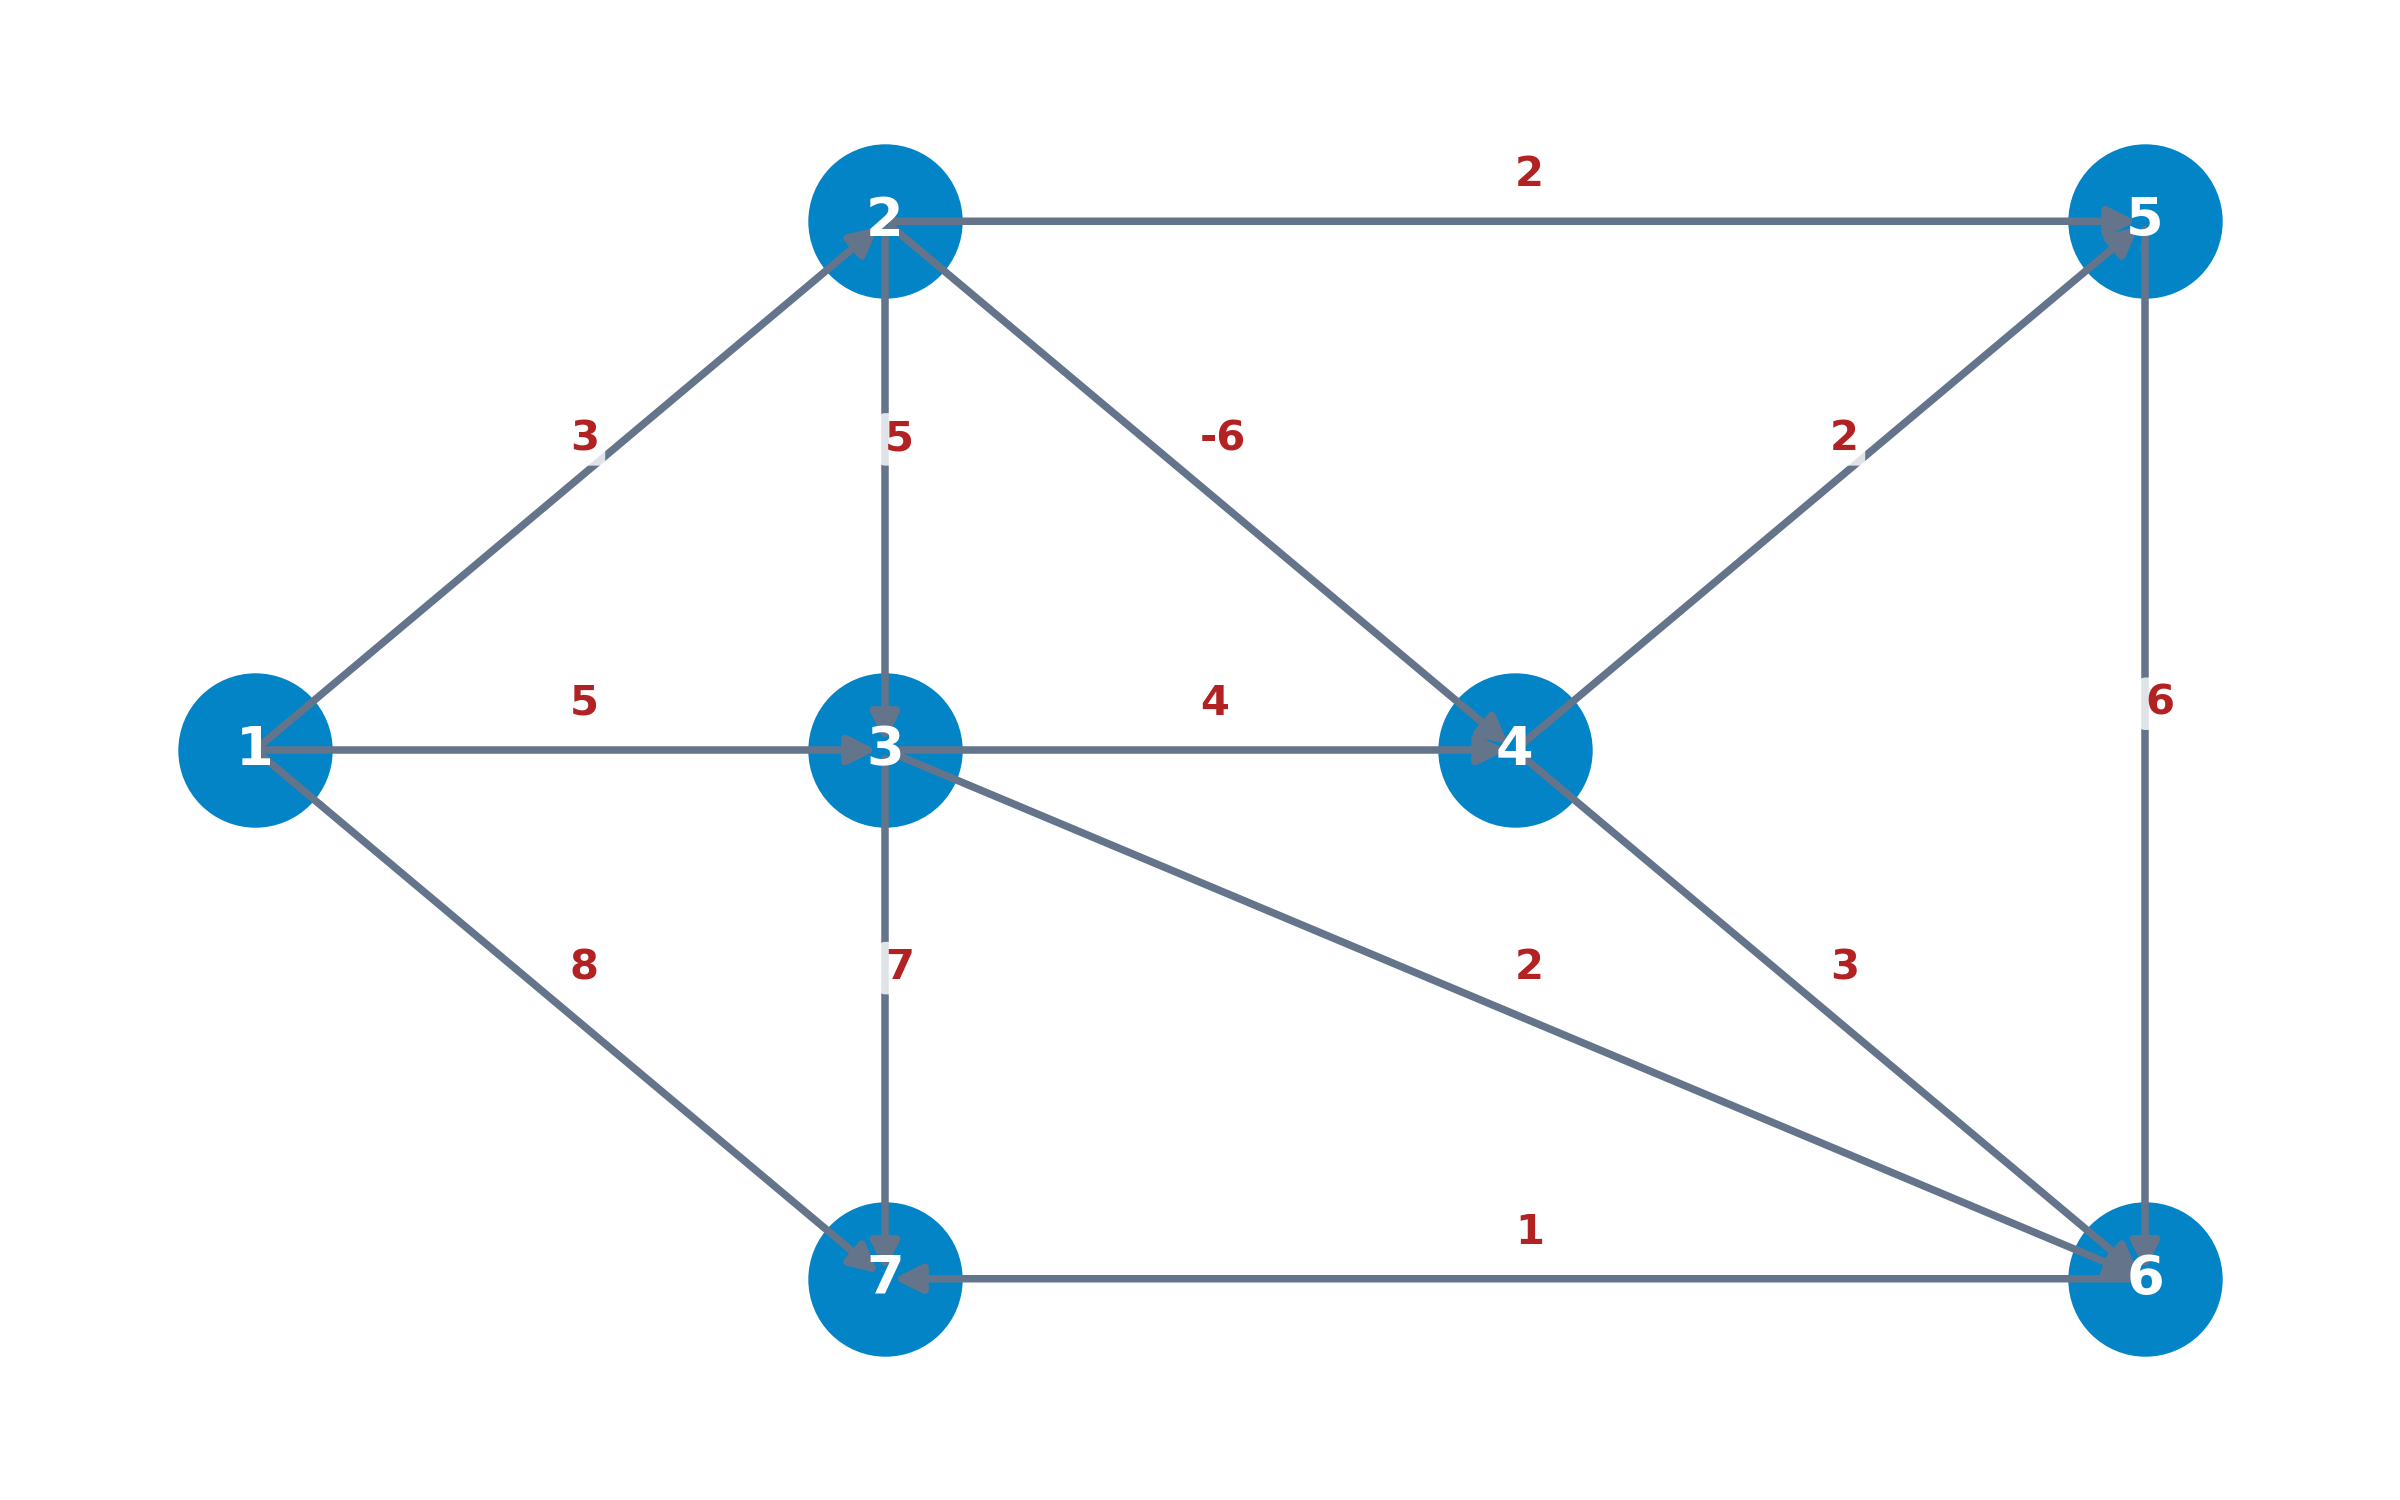
\includegraphics[width=0.85\linewidth,height=\textheight,keepaspectratio]{../images/dag_ejemplo_7nodos.png}
\end{center}
\end{frame}

\begin{frame}{Ejemplo DAG: Iteraciones analíticas nodo por nodo}
\phantomsection\label{ejemplo-dag-iteraciones-analuxedticas-nodo-por-nodo}
\begin{itemize}
\tightlist
\item
  \textbf{\(u_1 = 0\)} (Origen).
\item
  \textbf{\(u_2 = u_1 + d_{12} = 0 + 3 = 3\)} (\(\text{Pred}(2) = 1\)).
\item
  \textbf{\(u_3 = \min \{ u_1 + d_{13}, u_2 + d_{23} \} = \min \{ 0+5, 3+5 \} = 5\)}
  (\(\text{Pred}(3) = 1\)).
\item
  \textbf{\(u_4 = \min \{ u_2 + d_{24}, u_3 + d_{34} \} = \min \{ 3-6, 5+4 \} = -3\)}
  (\(\text{Pred}(4) = 2\)).
\item
  \textbf{\(u_5 = \min \{ u_2 + d_{25}, u_4 + d_{45} \} = \min \{ 3+2, -3+2 \} = -1\)}
  (\(\text{Pred}(5) = 4\)).
\item
  \textbf{\(u_6 = \min \{ u_3 + d_{36}, u_4 + d_{46}, u_5 + d_{56} \} = \min \{ 5+2, -3+3, -1+6 \} = 0\)}
  (\(\text{Pred}(6) = 4\)).
\item
  \textbf{\(u_7 = \min \{ u_1 + d_{17}, u_3 + d_{37}, u_6 + d_{67} \} = \min \{ 0+8, 5+7, 0+1 \} = 1\)}
  (\(\text{Pred}(7) = 6\)).
\end{itemize}
\end{frame}

\begin{frame}{Ejemplo DAG: Traza animada interactiva}
\phantomsection\label{ejemplo-dag-traza-animada-interactiva}
\end{frame}

\section{Redes con pesos no negativos: Algoritmo de
Dijkstra}\label{redes-con-pesos-no-negativos-algoritmo-de-dijkstra}

\begin{frame}{Filosofía del Algoritmo de Dijkstra (1959)}
\phantomsection\label{filosofuxeda-del-algoritmo-de-dijkstra-1959}
\begin{tcolorbox}[enhanced jigsaw, arc=.35mm, title=\textcolor{quarto-callout-note-color}{\faInfo}\hspace{0.5em}{Estrategia voraz de etiquetado permanente}, titlerule=0mm, opacitybacktitle=0.6, left=2mm, rightrule=.15mm, colback=white, colframe=quarto-callout-note-color-frame, toprule=.15mm, opacityback=0, coltitle=black, breakable, colbacktitle=quarto-callout-note-color!10!white, bottomtitle=1mm, leftrule=.75mm, bottomrule=.15mm, toptitle=1mm]

Para redes con costes no negativos (\(d_{ij} \ge 0\)), se dividen los
vértices en dos conjuntos:

\begin{itemize}
\tightlist
\item
  \textbf{Nodos Permanentes \(\mathcal{P}\)}: Vértices con distancia
  óptima definitiva conocida (\(u_j = d(1, j)\)).
\item
  \textbf{Nodos Transitorios \(\mathcal{T} = V \setminus \mathcal{P}\)}:
  Vértices con cota de distancia provisional \(u_j\).
\end{itemize}

\end{tcolorbox}

\begin{itemize}
\tightlist
\item
  \textbf{Mecanismo voraz (\emph{Greedy})}: En cada etapa se transfiere
  a \(\mathcal{P}\) el nodo \(k \in \mathcal{T}\) con etiqueta mínima:
  \[u_k = \min_{j \in \mathcal{T}} \{ u_j \}\]
\end{itemize}
\end{frame}

\begin{frame}{Definición de cota provisional \(u_j^P\)}
\phantomsection\label{definiciuxf3n-de-cota-provisional-u_jp}
\begin{tcolorbox}[enhanced jigsaw, arc=.35mm, title=\textcolor{quarto-callout-note-color}{\faInfo}\hspace{0.5em}{Cota de distancia provisional}, titlerule=0mm, opacitybacktitle=0.6, left=2mm, rightrule=.15mm, colback=white, colframe=quarto-callout-note-color-frame, toprule=.15mm, opacityback=0, coltitle=black, breakable, colbacktitle=quarto-callout-note-color!10!white, bottomtitle=1mm, leftrule=.75mm, bottomrule=.15mm, toptitle=1mm]

Dado el subconjunto permanente \(\mathcal{P}\), la cota \(u_j^P\)
asociada a un nodo \(j \in \mathcal{T}\) representa la longitud del
camino mínimo desde el origen \(1\) al nodo \(j\) utilizando como
vértices intermedios \textbf{únicamente elementos de \(\mathcal{P}\)}:

\[
u_j^P \equiv \text{distancia mínima de } 1 \text{ a } j \text{ pasando solo por } \mathcal{P}
\]

\end{tcolorbox}

\begin{itemize}
\tightlist
\item
  Al incorporar \(k\) a \(\mathcal{P}\), las cotas de los vecinos
  transitorios se actualizan mediante:
  \[u_j \leftarrow \min \{ u_j, \, u_k + d_{kj} \}\]
\end{itemize}
\end{frame}

\begin{frame}{Esquema del Algoritmo de Dijkstra}
\phantomsection\label{esquema-del-algoritmo-de-dijkstra}
\begin{tcolorbox}[enhanced jigsaw, arc=.35mm, title=\textcolor{quarto-callout-note-color}{\faInfo}\hspace{0.5em}{Algoritmo de Dijkstra}, titlerule=0mm, opacitybacktitle=0.6, left=2mm, rightrule=.15mm, colback=white, colframe=quarto-callout-note-color-frame, toprule=.15mm, opacityback=0, coltitle=black, breakable, colbacktitle=quarto-callout-note-color!10!white, bottomtitle=1mm, leftrule=.75mm, bottomrule=.15mm, toptitle=1mm]

Dada la red con costes no negativos \(d_{ij} \ge 0\):

\begin{enumerate}
\tightlist
\item
  \textbf{Paso 0 (Inicialización)}:

  \begin{itemize}
  \tightlist
  \item
    \(u_1 = 0\), \(u_j = d_{1j}\) (\(\forall j \ge 2\)),
    \(\mathcal{P} = \{1\}\), \(\mathcal{T} = \{2, \dots, n\}\),
    \(\text{Pred}(j) = 1\).
  \end{itemize}
\item
  \textbf{Paso 1 (Etiquetado permanente)}:

  \begin{itemize}
  \tightlist
  \item
    Seleccionar \(k \in \mathcal{T}\) tal que
    \(u_k = \min_{j \in \mathcal{T}} \{ u_j \}\).
  \item
    Hacer \(\mathcal{P} \leftarrow \mathcal{P} \cup \{k\}\),
    \(\mathcal{T} \leftarrow \mathcal{T} \setminus \{k\}\).
  \item
    Si \(\mathcal{T} = \emptyset\) o \(u_k = \infty\), \textbf{parar}.
  \end{itemize}
\item
  \textbf{Paso 2 (Relajación de etiquetas)}:

  \begin{itemize}
  \tightlist
  \item
    Para cada \(j \in \mathcal{T}\) vecino de \(k\):
    \(u_j \leftarrow \min \{ u_j, \, u_k + d_{kj} \}\). Si cambia, hacer
    \(\text{Pred}(j) \leftarrow k\). Ir al Paso 1.
  \end{itemize}
\end{enumerate}

\end{tcolorbox}
\end{frame}

\begin{frame}{Correctitud del Algoritmo de Dijkstra}
\phantomsection\label{correctitud-del-algoritmo-de-dijkstra}
\begin{tcolorbox}[enhanced jigsaw, arc=.35mm, title=\textcolor{quarto-callout-important-color}{\faExclamation}\hspace{0.5em}{Correctitud del algoritmo de Dijkstra}, titlerule=0mm, opacitybacktitle=0.6, left=2mm, rightrule=.15mm, colback=white, colframe=quarto-callout-important-color-frame, toprule=.15mm, opacityback=0, coltitle=black, breakable, colbacktitle=quarto-callout-important-color!10!white, bottomtitle=1mm, leftrule=.75mm, bottomrule=.15mm, toptitle=1mm]

Si \(d_{ij} \ge 0\) para todo \((i, j) \in U\), la etiqueta \(u_k\)
asignada por el Algoritmo de Dijkstra en el momento en que un nodo \(k\)
pasa a ser permanente
(\(\mathcal{P} \leftarrow \mathcal{P} \cup \{k\}\)) es la
\textbf{distancia mínima exacta} desde el origen \(1\) al nodo \(k\).

\end{tcolorbox}

\begin{itemize}
\tightlist
\item
  \textbf{Interpretación y fundamento de la no negatividad}:

  \begin{itemize}
  \tightlist
  \item
    Como \(d_{ij} \ge 0\), la función de distancia a lo largo de
    cualquier camino es \textbf{monótona no decreciente}.
  \item
    Ningún camino que atraviese un nodo transitorio
    \(y \in \mathcal{T}\) puede ofrecer un coste menor que la etiqueta
    mínima \(u_k = \min_{j \in \mathcal{T}} \{ u_j \}\).
  \item
    Al pasar \(k\) a permanente, su distancia \(u_k\) queda
    \textbf{definitivamente fijada y garantizada como óptima}.
  \end{itemize}
\end{itemize}
\end{frame}

\begin{frame}{Complejidad computacional de Dijkstra}
\phantomsection\label{complejidad-computacional-de-dijkstra}
\begin{longtable}[]{@{}
  >{\raggedright\arraybackslash}p{(\linewidth - 4\tabcolsep) * \real{0.3333}}
  >{\raggedright\arraybackslash}p{(\linewidth - 4\tabcolsep) * \real{0.3333}}
  >{\raggedright\arraybackslash}p{(\linewidth - 4\tabcolsep) * \real{0.3333}}@{}}
\toprule\noalign{}
\begin{minipage}[b]{\linewidth}\raggedright
Estructura de Datos
\end{minipage} & \begin{minipage}[b]{\linewidth}\raggedright
Complejidad Temporal
\end{minipage} & \begin{minipage}[b]{\linewidth}\raggedright
Contexto de Aplicación
\end{minipage} \\
\midrule\noalign{}
\endhead
\textbf{Matriz de distancias} & \(O(n^2)\) & Redes densas
(\(m \approx n^2\)) \\
\textbf{Heap binario (Min-Heap)} & \(O(m \log n)\) & Redes dispersas
(\(m \ll n^2\)) \\
\textbf{Fibonacci Heap} & \textbf{\(O(m + n \log n)\)} & Máxima
eficiencia teórica \\
\bottomrule\noalign{}
\end{longtable}

\begin{itemize}
\tightlist
\item
  \textbf{Justificación de la voracidad}: Si \(d_{ij} \ge 0\), ningún
  nodo en \(\mathcal{T}\) puede ofrecer un camino más corto hacia \(k\)
  que la propia cota actual
  \(u_k = \min_{j \in \mathcal{T}} \{ u_j \}\).
\end{itemize}
\end{frame}

\begin{frame}{Ejemplo Dijkstra: Red de 5 nodos}
\phantomsection\label{ejemplo-dijkstra-red-de-5-nodos}
\begin{columns}[T]
\begin{column}{0.5\linewidth}
\begin{center}
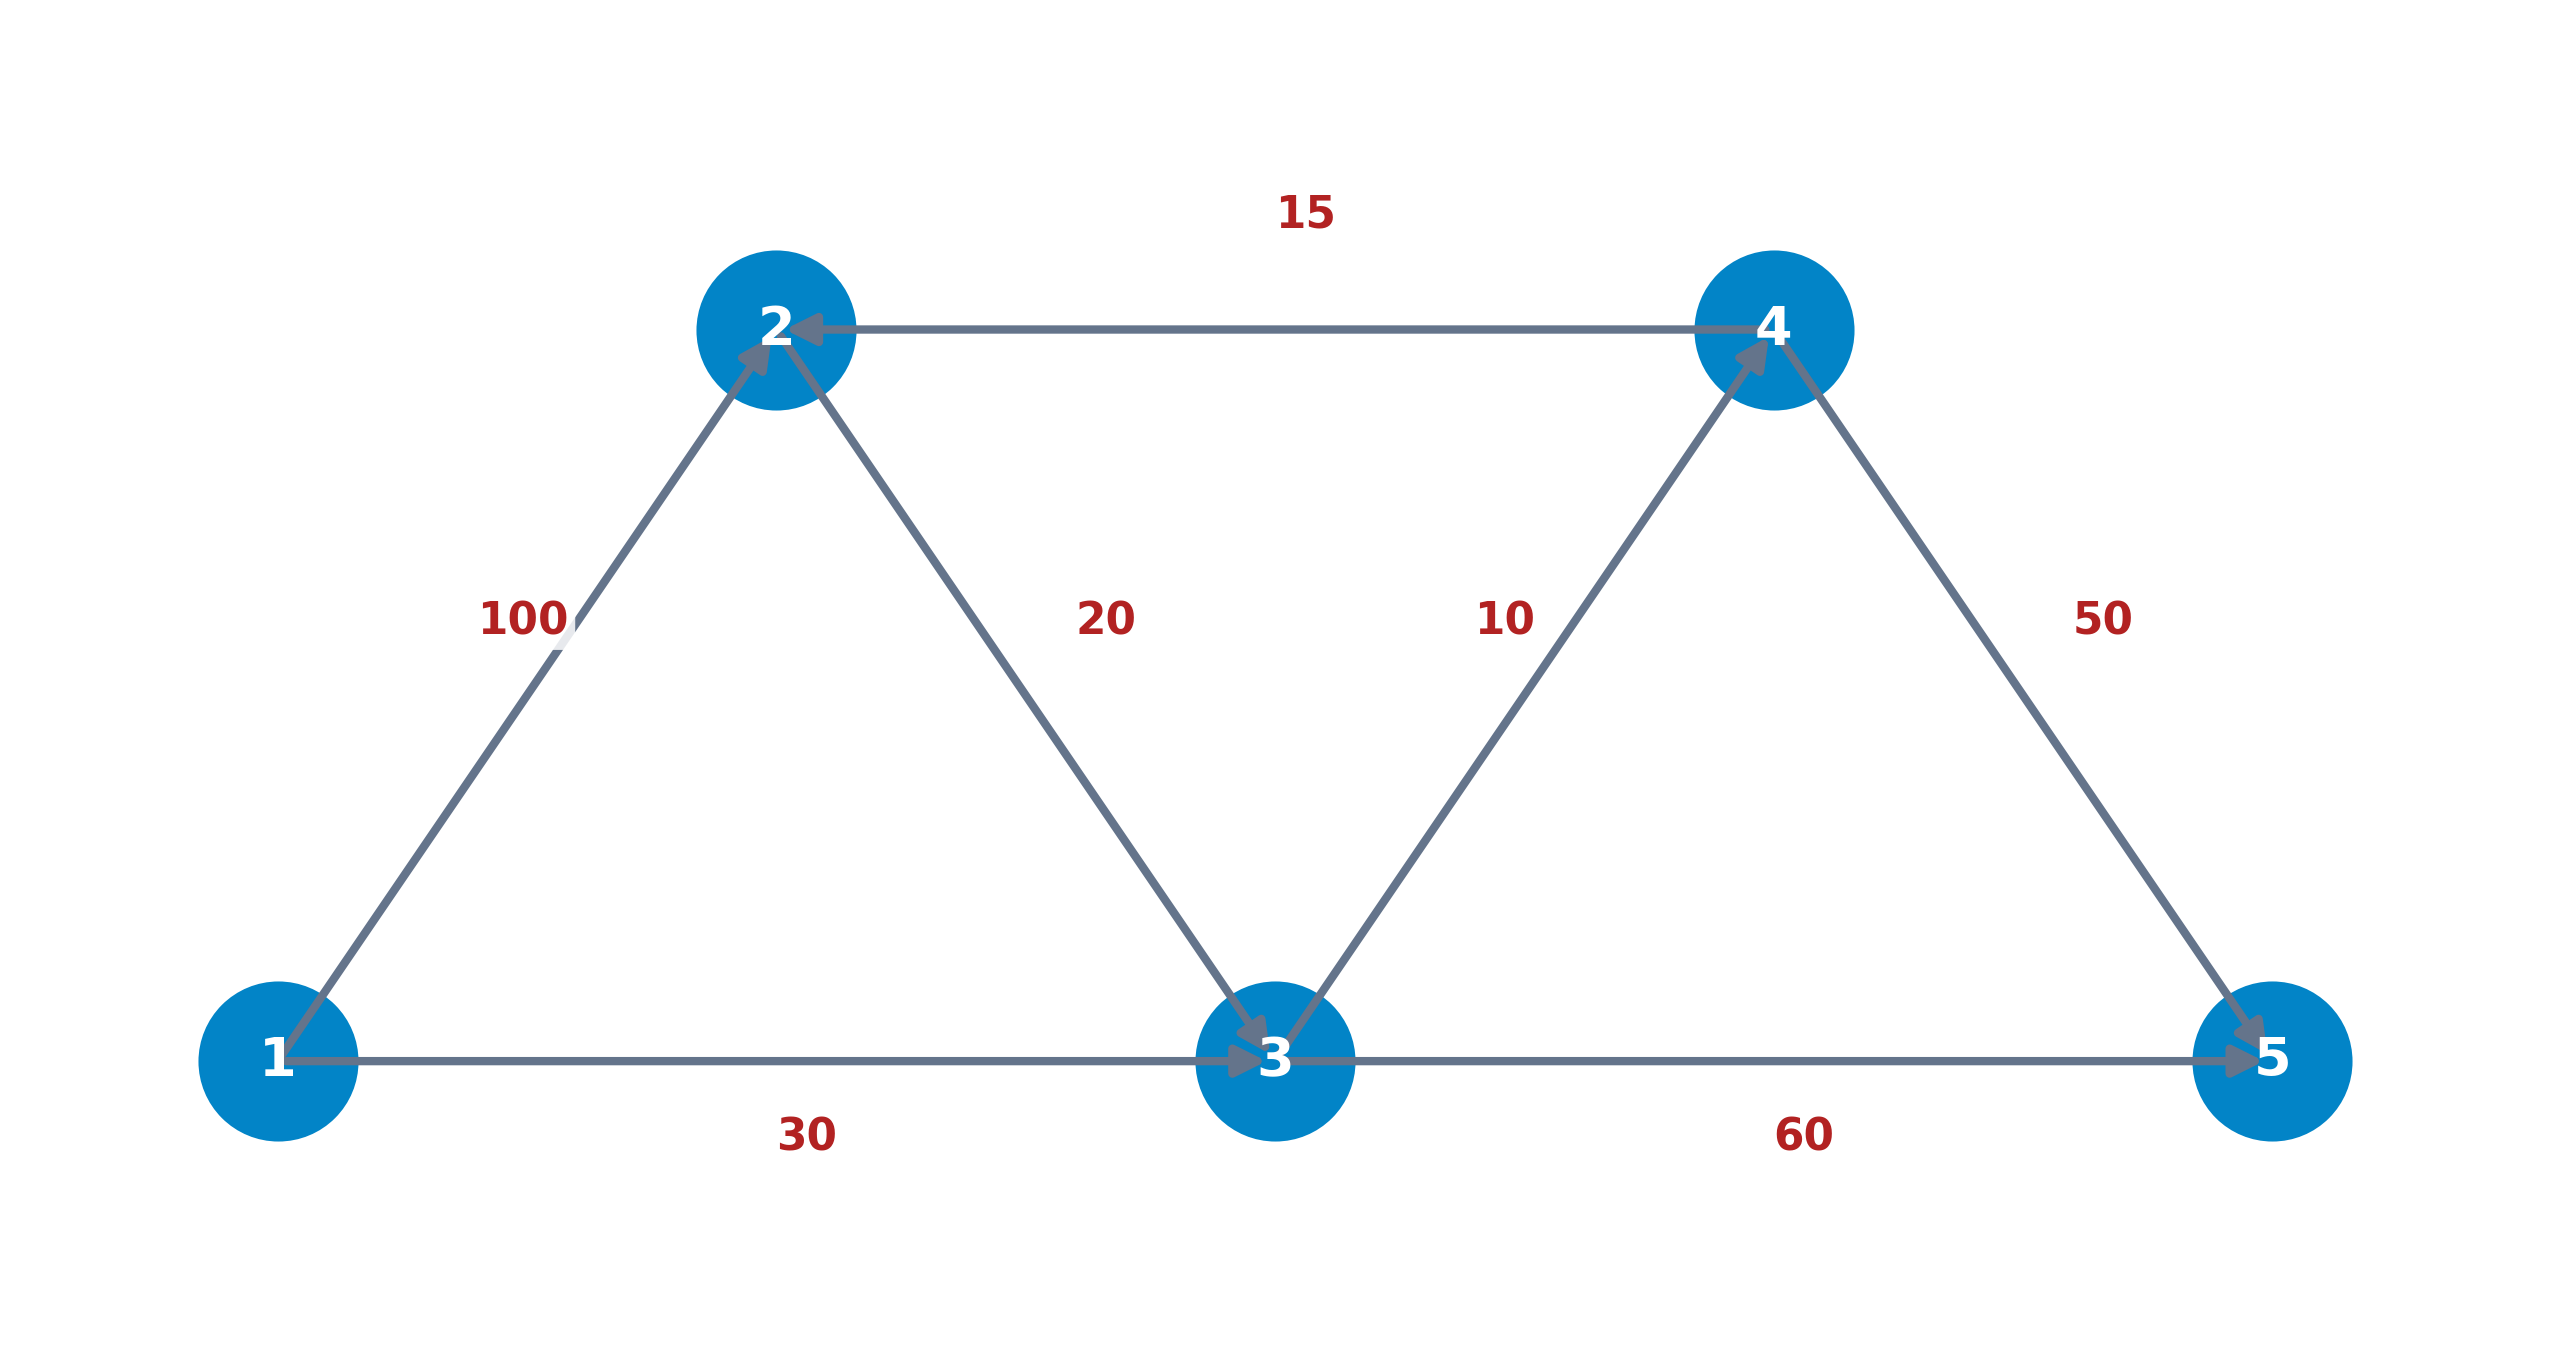
\includegraphics[width=0.95\linewidth,height=\textheight,keepaspectratio]{../images/dijkstra_ejemplo_5nodos.png}
\end{center}
\end{column}

\begin{column}{0.5\linewidth}
\begin{itemize}
\item
  \textbf{Digrafo de 5 nodos}: Costes estrictamente no negativos.
\item
  \textbf{Objetivo}: Determinar el árbol de caminos mínimos desde el
  nodo origen 1.
\end{itemize}
\end{column}
\end{columns}
\end{frame}

\begin{frame}{Ejemplo Dijkstra: Iteración 0 e Iteración 1}
\phantomsection\label{ejemplo-dijkstra-iteraciuxf3n-0-e-iteraciuxf3n-1}
\begin{itemize}
\tightlist
\item
  \textbf{Paso 0 (Inicialización)}:

  \begin{itemize}
  \tightlist
  \item
    \(\mathcal{P} = \{1\}\), \(\mathcal{T} = \{2, 3, 4, 5\}\).
  \item
    \(u = (0, 100, 30, \infty, \infty)\),
    \(\text{Pred} = (1, 1, 1, 1, 1)\).
  \end{itemize}
\item
  \textbf{Iteración 1}:

  \begin{itemize}
  \tightlist
  \item
    Mínimo en \(\mathcal{T}\): \(k = 3\) con
    \(u_3 = 30 \implies \mathcal{P} = \{1, 3\}\),
    \(\mathcal{T} = \{2, 4, 5\}\).
  \item
    Relajación de vecinos de 3:

    \begin{itemize}
    \tightlist
    \item
      \(u_2 \leftarrow \min \{100, 30 + 20\} = 50\)
      (\(\text{Pred}(2) = 3\)).
    \item
      \(u_4 \leftarrow \min \{\infty, 30 + 10\} = 40\)
      (\(\text{Pred}(4) = 3\)).
    \item
      \(u_5 \leftarrow \min \{\infty, 30 + 60\} = 90\)
      (\(\text{Pred}(5) = 3\)).
    \end{itemize}
  \end{itemize}
\end{itemize}
\end{frame}

\begin{frame}{Ejemplo Dijkstra: Iteraciones 2 a 4}
\phantomsection\label{ejemplo-dijkstra-iteraciones-2-a-4}
\begin{itemize}
\tightlist
\item
  \textbf{Iteración 2}:

  \begin{itemize}
  \tightlist
  \item
    Mínimo en \(\mathcal{T}\): \(k = 4\) con
    \(u_4 = 40 \implies \mathcal{P} = \{1, 3, 4\}\),
    \(\mathcal{T} = \{2, 5\}\).
  \item
    Vecinos de 4: (arco \((4,2)\) peso 15: \(40+15=55 > 50\), sin
    cambio; \((4,5)\) peso 50: \(40+50=90\), sin cambio).
  \end{itemize}
\item
  \textbf{Iteración 3}:

  \begin{itemize}
  \tightlist
  \item
    Mínimo en \(\mathcal{T}\): \(k = 2\) con
    \(u_2 = 50 \implies \mathcal{P} = \{1, 3, 4, 2\}\),
    \(\mathcal{T} = \{5\}\).
  \end{itemize}
\item
  \textbf{Iteración 4}:

  \begin{itemize}
  \tightlist
  \item
    Mínimo en \(\mathcal{T}\): \(k = 5\) con
    \(u_5 = 90 \implies \mathcal{P} = \{1, 2, 3, 4, 5\}\),
    \(\mathcal{T} = \emptyset\). \textbf{PARADA}.
  \end{itemize}
\end{itemize}
\end{frame}

\begin{frame}{Ejemplo Dijkstra: Tabla resumen de desarrollo}
\phantomsection\label{ejemplo-dijkstra-tabla-resumen-de-desarrollo}
\begin{longtable}[]{@{}
  >{\raggedright\arraybackslash}p{(\linewidth - 10\tabcolsep) * \real{0.1667}}
  >{\raggedright\arraybackslash}p{(\linewidth - 10\tabcolsep) * \real{0.1667}}
  >{\raggedright\arraybackslash}p{(\linewidth - 10\tabcolsep) * \real{0.1667}}
  >{\raggedright\arraybackslash}p{(\linewidth - 10\tabcolsep) * \real{0.1667}}
  >{\raggedright\arraybackslash}p{(\linewidth - 10\tabcolsep) * \real{0.1667}}
  >{\raggedright\arraybackslash}p{(\linewidth - 10\tabcolsep) * \real{0.1667}}@{}}
\toprule\noalign{}
\begin{minipage}[b]{\linewidth}\raggedright
Etapa \(k\)
\end{minipage} & \begin{minipage}[b]{\linewidth}\raggedright
Nodo Permanetizado
\end{minipage} & \begin{minipage}[b]{\linewidth}\raggedright
\(u_k\)
\end{minipage} & \begin{minipage}[b]{\linewidth}\raggedright
Conjunto \(\mathcal{P}\)
\end{minipage} & \begin{minipage}[b]{\linewidth}\raggedright
Etiquetas \((u_1, u_2, u_3, u_4, u_5)\)
\end{minipage} & \begin{minipage}[b]{\linewidth}\raggedright
Predecesores \(\text{Pred}(1..5)\)
\end{minipage} \\
\midrule\noalign{}
\endhead
\textbf{Inicio} & \(1\) & \(0\) & \(\{1\}\) &
\((0, 100, 30, \infty, \infty)\) & \((1, 1, 1, 1, 1)\) \\
\textbf{Iter 1} & \(3\) & \(30\) & \(\{1, 3\}\) &
\((0, 50, 30, 40, 90)\) & \((1, 3, 1, 3, 3)\) \\
\textbf{Iter 2} & \(4\) & \(40\) & \(\{1, 3, 4\}\) &
\((0, 50, 30, 40, 90)\) & \((1, 3, 1, 3, 3)\) \\
\textbf{Iter 3} & \(2\) & \(50\) & \(\{1, 3, 4, 2\}\) &
\((0, 50, 30, 40, 90)\) & \((1, 3, 1, 3, 3)\) \\
\textbf{Iter 4} & \(5\) & \(90\) & \(\{1, 3, 4, 2, 5\}\) &
\((0, 50, 30, 40, 90)\) & \((1, 3, 1, 3, 3)\) \\
\bottomrule\noalign{}
\end{longtable}

\begin{itemize}
\tightlist
\item
  \textbf{Arborescencia Óptima}: \(\{ (1,3), (3,4), (3,2), (3,5) \}\).
\end{itemize}
\end{frame}

\begin{frame}{Ejemplo Dijkstra: Traza animada interactiva}
\phantomsection\label{ejemplo-dijkstra-traza-animada-interactiva}
\end{frame}

\section{Redes con pesos negativos: Algoritmo de
Bellman-Ford}\label{redes-con-pesos-negativos-algoritmo-de-bellman-ford}

\begin{frame}{Concepto: Aproximación por número de arcos (1956-1959)}
\phantomsection\label{concepto-aproximaciuxf3n-por-nuxfamero-de-arcos-1956-1959}
\begin{tcolorbox}[enhanced jigsaw, arc=.35mm, title=\textcolor{quarto-callout-note-color}{\faInfo}\hspace{0.5em}{Aproximación iterativa por longitud de arcos}, titlerule=0mm, opacitybacktitle=0.6, left=2mm, rightrule=.15mm, colback=white, colframe=quarto-callout-note-color-frame, toprule=.15mm, opacityback=0, coltitle=black, breakable, colbacktitle=quarto-callout-note-color!10!white, bottomtitle=1mm, leftrule=.75mm, bottomrule=.15mm, toptitle=1mm]

Para redes que contienen arcos con costes negativos (sin circuitos
negativos), el \textbf{Algoritmo de Bellman-Ford} define:

\begin{itemize}
\item
  \textbf{Etiqueta \(u_j^m\)}: Longitud del camino mínimo desde el
  origen \(1\) al nodo \(j\) utilizando \textbf{a lo sumo \(m\) arcos}.
\item
  \textbf{Relación de Recurrencia}:
  \[u_j^m = \min \left\{ u_j^{m-1}, \ \min_{k \neq j} \{ u_k^{m-1} + d_{kj} \} \right\}, \quad m = 1, \dots, n-1\]
\end{itemize}

\end{tcolorbox}

\begin{itemize}
\tightlist
\item
  \textbf{Complejidad}: \(O(|V| \cdot |U|) = O(n^3)\) para redes densas.
\end{itemize}
\end{frame}

\begin{frame}{Esquema del Algoritmo de Bellman-Ford (I: Inicialización)}
\phantomsection\label{esquema-del-algoritmo-de-bellman-ford-i-inicializaciuxf3n}
\begin{tcolorbox}[enhanced jigsaw, arc=.35mm, title=\textcolor{quarto-callout-note-color}{\faInfo}\hspace{0.5em}{Algoritmo de Bellman-Ford --- Paso 1: Inicialización}, titlerule=0mm, opacitybacktitle=0.6, left=2mm, rightrule=.15mm, colback=white, colframe=quarto-callout-note-color-frame, toprule=.15mm, opacityback=0, coltitle=black, breakable, colbacktitle=quarto-callout-note-color!10!white, bottomtitle=1mm, leftrule=.75mm, bottomrule=.15mm, toptitle=1mm]

Dada una red valorada dirigida \(G = (V, U, \mathbf{d})\) con
\(n = |V|\) vértices:

\begin{itemize}
\tightlist
\item
  \textbf{Paso 1 (Inicialización para \(m = 1\))}: Definir las etiquetas
  iniciales de distancia directa desde el origen \(1\): \[
  u_j^1 = \begin{cases} 
  0 & \text{si } j = 1 \\ 
  d_{1j} & \text{si } (1, j) \in U \\ 
  \infty & \text{si } (1, j) \notin U 
  \end{cases}
  \] y establecer el vector de predecesores iniciales
  \(\text{Pred}(j) = 1\). Inicializar el contador de arcos:
  \(m \leftarrow 1\).
\end{itemize}

\end{tcolorbox}
\end{frame}

\begin{frame}{Esquema del Algoritmo de Bellman-Ford (II: Relajación)}
\phantomsection\label{esquema-del-algoritmo-de-bellman-ford-ii-relajaciuxf3n}
\begin{tcolorbox}[enhanced jigsaw, arc=.35mm, title=\textcolor{quarto-callout-note-color}{\faInfo}\hspace{0.5em}{Algoritmo de Bellman-Ford --- Paso 2: Relajación de arcos}, titlerule=0mm, opacitybacktitle=0.6, left=2mm, rightrule=.15mm, colback=white, colframe=quarto-callout-note-color-frame, toprule=.15mm, opacityback=0, coltitle=black, breakable, colbacktitle=quarto-callout-note-color!10!white, bottomtitle=1mm, leftrule=.75mm, bottomrule=.15mm, toptitle=1mm]

\begin{itemize}
\tightlist
\item
  \textbf{Paso 2 (Iteración de relajación)}:

  \begin{itemize}
  \tightlist
  \item
    Incrementar la longitud máxima permitida del camino:
    \(m \leftarrow m + 1\).
  \item
    Para cada nodo \(j = 2, \dots, n\), evaluar si es más ventajoso
    mantener la cota anterior o acceder a \(j\) pasando por un nodo
    intermedio \(k\): \[
    u_j^m = \min \left\{ u_j^{m-1}, \ \min_{k \neq j} \{ u_k^{m-1} + d_{kj} \} \right\}
    \]
  \item
    Si la etiqueta cambia (\(u_j^m < u_j^{m-1}\)), actualizar el
    predecesor: \(\text{Pred}(j) \leftarrow k\).
  \end{itemize}
\end{itemize}

\end{tcolorbox}
\end{frame}

\begin{frame}{Esquema del Algoritmo de Bellman-Ford (III: Parada)}
\phantomsection\label{esquema-del-algoritmo-de-bellman-ford-iii-parada}
\begin{tcolorbox}[enhanced jigsaw, arc=.35mm, title=\textcolor{quarto-callout-note-color}{\faInfo}\hspace{0.5em}{Algoritmo de Bellman-Ford --- Paso 3: Criterios de Parada}, titlerule=0mm, opacitybacktitle=0.6, left=2mm, rightrule=.15mm, colback=white, colframe=quarto-callout-note-color-frame, toprule=.15mm, opacityback=0, coltitle=black, breakable, colbacktitle=quarto-callout-note-color!10!white, bottomtitle=1mm, leftrule=.75mm, bottomrule=.15mm, toptitle=1mm]

\begin{itemize}
\item
  \textbf{Paso 3 (Criterio de Parada y Convergencia)}:

  \begin{itemize}
  \item
    \textbf{Parada Anticipada (Estabilidad)}: Si \(u_j^m = u_j^{m-1}\)
    para todo \(j = 2, \dots, n\), la solución es \textbf{óptima y
    estable} \(\implies\) \textbf{PARAR}.
  \item
    \textbf{Criterio Límite (\(m = n - 1\))}: Si \(m = n - 1\), se ha
    alcanzado el número máximo de arcos de un camino simple \(\implies\)
    \textbf{PARAR}.
  \item
    \textbf{Continuación}: Si \(m < n - 1\) y \(u^m \neq u^{m-1}\),
    \textbf{regresar al Paso 2}.
  \end{itemize}
\end{itemize}

\end{tcolorbox}

\begin{itemize}
\tightlist
\item
  \textbf{Interpretación teórica}: Cualquier camino simple entre dos
  nodos contiene a lo sumo \(n-1\) arcos. Si la red no posee circuitos
  de coste negativo, la solución óptima se alcanza en \(m \le n-1\)
  iteraciones.
\end{itemize}
\end{frame}

\begin{frame}{Ejemplo Bellman-Ford: Red de 4 nodos con costes negativos}
\phantomsection\label{ejemplo-bellman-ford-red-de-4-nodos-con-costes-negativos}
\begin{columns}[T]
\begin{column}{0.5\linewidth}
\begin{center}
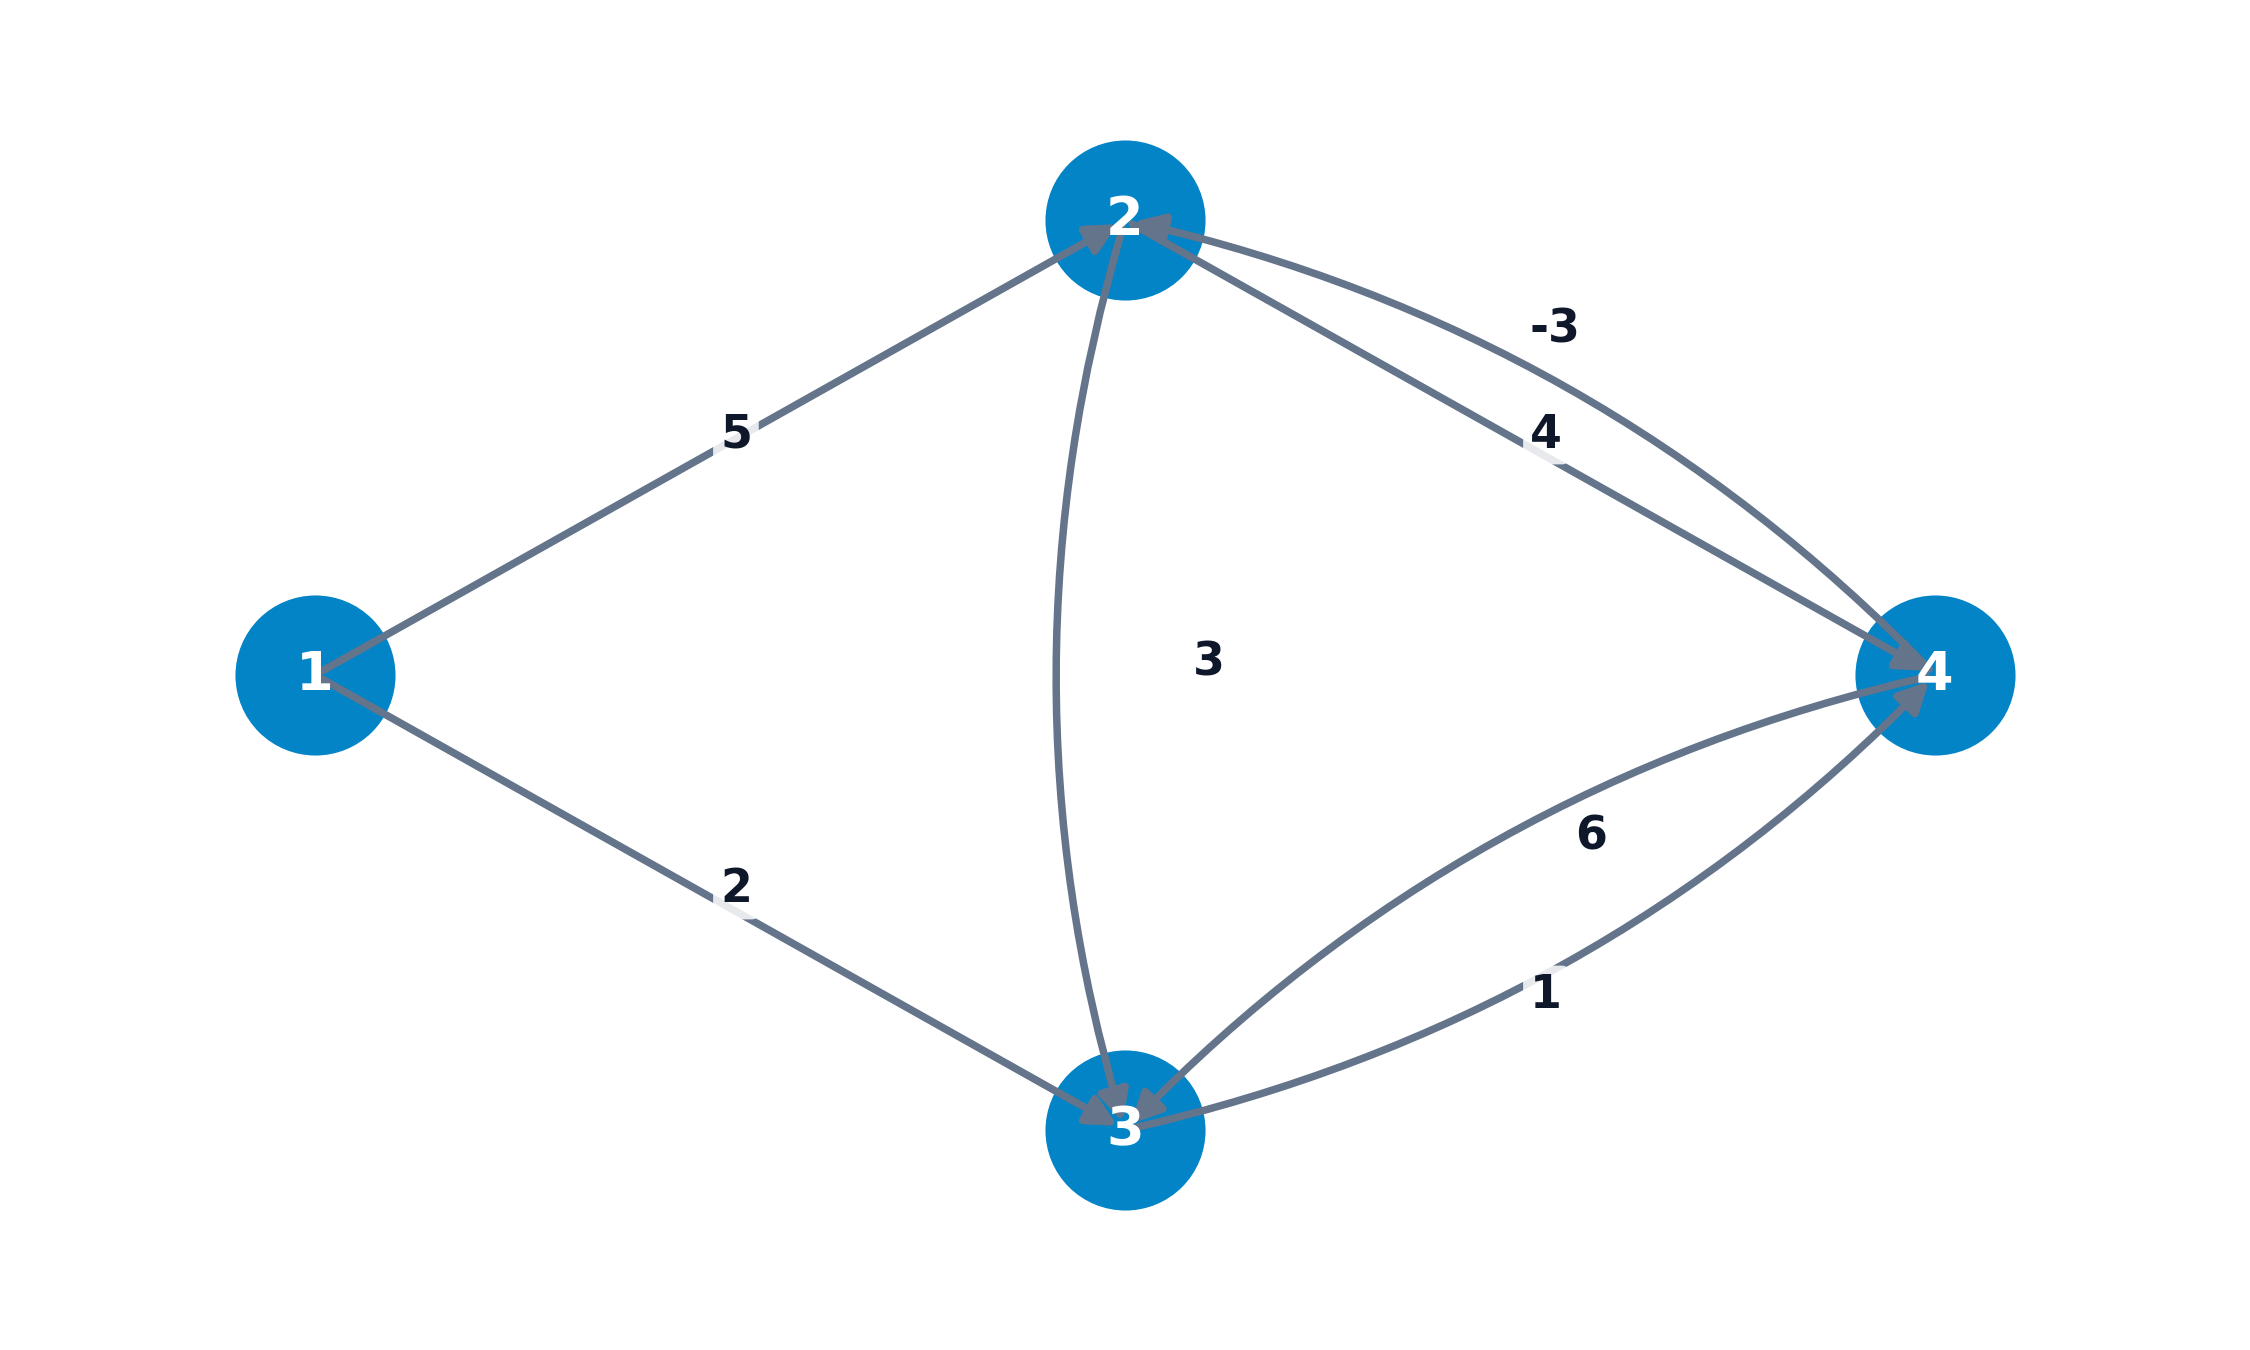
\includegraphics[width=0.95\linewidth,height=\textheight,keepaspectratio]{../images/bellman_ford_ejemplo_4nodos.png}
\end{center}
\end{column}

\begin{column}{0.5\linewidth}
\begin{itemize}
\item
  \textbf{Arco negativo}: \((4, 2)\) con coste \(d_{42} = -3\).
\item
  \textbf{Objetivo}: Obtener las distancias mínimas desde el nodo 1.
\end{itemize}
\end{column}
\end{columns}
\end{frame}

\begin{frame}{Ejemplo Bellman-Ford: Desarrollo iterativo m=1 y m=2}
\phantomsection\label{ejemplo-bellman-ford-desarrollo-iterativo-m1-y-m2}
\begin{itemize}
\tightlist
\item
  \textbf{Paso 1 (\(m=1\))}:

  \begin{itemize}
  \tightlist
  \item
    \(u^1 = (0, 5, 2, \infty)\), \(\text{Pred} = (1, 1, 1, 1)\).
  \end{itemize}
\item
  \textbf{Iteración \(m=2\)}:

  \begin{itemize}
  \tightlist
  \item
    \(u_2^2 = \min \{ u_2^1, u_3^1 + d_{32}, u_4^1 + d_{42} \} = \min \{ 5, 2+\infty, \infty-3 \} = 5\).
  \item
    \(u_3^2 = \min \{ u_3^1, u_2^1 + d_{23}, u_4^1 + d_{43} \} = \min \{ 2, 5+3, \infty+6 \} = 2\).
  \item
    \(u_4^2 = \min \{ u_4^1, u_2^1 + d_{24}, u_3^1 + d_{34} \} = \min \{ \infty, 5+4, 2+1 \} = 3\).
  \item
    Vector resultante: \(u^2 = (0, 5, 2, 3)\),
    \(\text{Pred} = (1, 1, 1, 3)\).
  \end{itemize}
\end{itemize}
\end{frame}

\begin{frame}{Ejemplo Bellman-Ford: Desarrollo iterativo m=3 y m=4}
\phantomsection\label{ejemplo-bellman-ford-desarrollo-iterativo-m3-y-m4}
\begin{itemize}
\tightlist
\item
  \textbf{Iteración \(m=3\)}:

  \begin{itemize}
  \tightlist
  \item
    \(u_2^3 = \min \{ 5, u_3^2 + d_{32}, u_4^2 + d_{42} \} = \min \{ 5, 2+\infty, 3 - 3 \} = 0\)
    (\(\text{Pred}(2) = 4\)).
  \item
    \(u_3^3 = \min \{ 2, u_2^2 + d_{23}, u_4^2 + d_{43} \} = \min \{ 2, 5+3, 3+6 \} = 2\).
  \item
    \(u_4^3 = \min \{ 3, u_2^2 + d_{24}, u_3^2 + d_{34} \} = \min \{ 3, 5+4, 2+1 \} = 3\).
  \item
    Vector resultante: \(u^3 = (0, 0, 2, 3)\),
    \(\text{Pred} = (1, 4, 1, 3)\).
  \end{itemize}
\item
  \textbf{Iteración \(m=4\)}:

  \begin{itemize}
  \tightlist
  \item
    \(u^4 = (0, 0, 2, 3) = u^3 \implies\) \textbf{CONVERGENCIA
    ALCANZADA}.
  \end{itemize}
\end{itemize}
\end{frame}

\begin{frame}{Ejemplo Bellman-Ford: Tabla resumen de iteraciones}
\phantomsection\label{ejemplo-bellman-ford-tabla-resumen-de-iteraciones}
\begin{longtable}[]{@{}
  >{\raggedright\arraybackslash}p{(\linewidth - 12\tabcolsep) * \real{0.1429}}
  >{\raggedright\arraybackslash}p{(\linewidth - 12\tabcolsep) * \real{0.1429}}
  >{\raggedright\arraybackslash}p{(\linewidth - 12\tabcolsep) * \real{0.1429}}
  >{\raggedright\arraybackslash}p{(\linewidth - 12\tabcolsep) * \real{0.1429}}
  >{\raggedright\arraybackslash}p{(\linewidth - 12\tabcolsep) * \real{0.1429}}
  >{\raggedright\arraybackslash}p{(\linewidth - 12\tabcolsep) * \real{0.1429}}
  >{\raggedright\arraybackslash}p{(\linewidth - 12\tabcolsep) * \real{0.1429}}@{}}
\toprule\noalign{}
\begin{minipage}[b]{\linewidth}\raggedright
Iteración \(m\)
\end{minipage} & \begin{minipage}[b]{\linewidth}\raggedright
\(u_1^m\)
\end{minipage} & \begin{minipage}[b]{\linewidth}\raggedright
\(u_2^m\)
\end{minipage} & \begin{minipage}[b]{\linewidth}\raggedright
\(u_3^m\)
\end{minipage} & \begin{minipage}[b]{\linewidth}\raggedright
\(u_4^m\)
\end{minipage} & \begin{minipage}[b]{\linewidth}\raggedright
Vector de Predecesores \(\text{Pred}\)
\end{minipage} & \begin{minipage}[b]{\linewidth}\raggedright
Estado de Convergencia
\end{minipage} \\
\midrule\noalign{}
\endhead
\textbf{\(m=1\)} & \(0\) & \(5\) & \(2\) & \(\infty\) & \((1, 1, 1, 1)\)
& Inicialización \\
\textbf{\(m=2\)} & \(0\) & \(5\) & \(2\) & \(3\) & \((1, 1, 1, 3)\) &
Relajación de \(u_4\) \\
\textbf{\(m=3\)} & \(0\) & \textbf{\(0\)} & \(2\) & \(3\) &
\((1, 4, 1, 3)\) & Relajación de \(u_2\) vía \((4,2)\) \\
\textbf{\(m=4\)} & \(0\) & \(0\) & \(2\) & \(3\) & \((1, 4, 1, 3)\) &
\(u^4 = u^3 \implies\) \textbf{Parada} \\
\bottomrule\noalign{}
\end{longtable}

\begin{itemize}
\tightlist
\item
  \textbf{Distancias Óptimas}: \(\mathbf{u}^* = (0, 0, 2, 3)\).
\item
  \textbf{Arborescencia}: \(\{ (1,3), (3,4), (4,2) \}\).
\end{itemize}
\end{frame}

\begin{frame}{Ejemplo Bellman-Ford: Traza animada interactiva}
\phantomsection\label{ejemplo-bellman-ford-traza-animada-interactiva}
\end{frame}

\begin{frame}{Detección de circuitos de coste negativo}
\phantomsection\label{detecciuxf3n-de-circuitos-de-coste-negativo}
\begin{tcolorbox}[enhanced jigsaw, arc=.35mm, title=\textcolor{quarto-callout-important-color}{\faExclamation}\hspace{0.5em}{Criterio de detección de circuitos de coste negativo}, titlerule=0mm, opacitybacktitle=0.6, left=2mm, rightrule=.15mm, colback=white, colframe=quarto-callout-important-color-frame, toprule=.15mm, opacityback=0, coltitle=black, breakable, colbacktitle=quarto-callout-important-color!10!white, bottomtitle=1mm, leftrule=.75mm, bottomrule=.15mm, toptitle=1mm]

Existe un circuito de coste negativo accesible desde el origen si y sólo
si en la iteración \(m = n\):

\[u_j^n \neq u_j^{n-1} \quad \text{para algún } j \in V\]

\end{tcolorbox}

\begin{itemize}
\tightlist
\item
  \textbf{Fundamento teórico}: Si no existen circuitos negativos, las
  distancias mínimas se alcanzan en a lo sumo \(n-1\) arcos. Si la
  iteración \(n\) modifica alguna distancia (\(u^n \neq u^{n-1}\)),
  existe un circuito de peso estrictamente negativo.
\end{itemize}
\end{frame}

\begin{frame}{Esquema: Algoritmo de Bellman-Ford adaptado}
\phantomsection\label{esquema-algoritmo-de-bellman-ford-adaptado}
\begin{tcolorbox}[enhanced jigsaw, arc=.35mm, title=\textcolor{quarto-callout-note-color}{\faInfo}\hspace{0.5em}{Algoritmo adaptado para detección de circuitos negativos}, titlerule=0mm, opacitybacktitle=0.6, left=2mm, rightrule=.15mm, colback=white, colframe=quarto-callout-note-color-frame, toprule=.15mm, opacityback=0, coltitle=black, breakable, colbacktitle=quarto-callout-note-color!10!white, bottomtitle=1mm, leftrule=.75mm, bottomrule=.15mm, toptitle=1mm]

Dada una red valorada general \(G = (V, U, \mathbf{d})\) con \(n = |V|\)
vértices:

\begin{enumerate}
\tightlist
\item
  \textbf{Inicialización (\(m=1\))}: \(u_1^1 = 0\), \(u_j^1 = d_{1j}\)
  (\(\forall j \ge 2\)), \(m \leftarrow 1\).
\item
  \textbf{Relajación iterativa}: Hacer \(m \leftarrow m + 1\). Para cada
  nodo \(j = 2, \dots, n\):
  \[u_j^m = \min \left\{ u_j^{m-1}, \, \min_{k \neq j} \{ u_k^{m-1} + d_{kj} \} \right\}\]
\item
  \textbf{Criterio de parada}:

  \begin{itemize}
  \tightlist
  \item
    Si \(u^m = u^{m-1}\), \textbf{PARAR}: Solución óptima alcanzada.
  \item
    Si \(m = n\) y \(u^n \neq u^{n-1}\), \textbf{PARAR}: Existen
    circuitos de coste negativo.
  \item
    En otro caso (\(m < n\)), regresar al Paso 2.
  \end{itemize}
\end{enumerate}

\end{tcolorbox}
\end{frame}

\begin{frame}{Ejemplo: Detección de circuito negativo (7 nodos)}
\phantomsection\label{ejemplo-detecciuxf3n-de-circuito-negativo-7-nodos}
\begin{columns}[T]
\begin{column}{0.45\linewidth}
\begin{center}
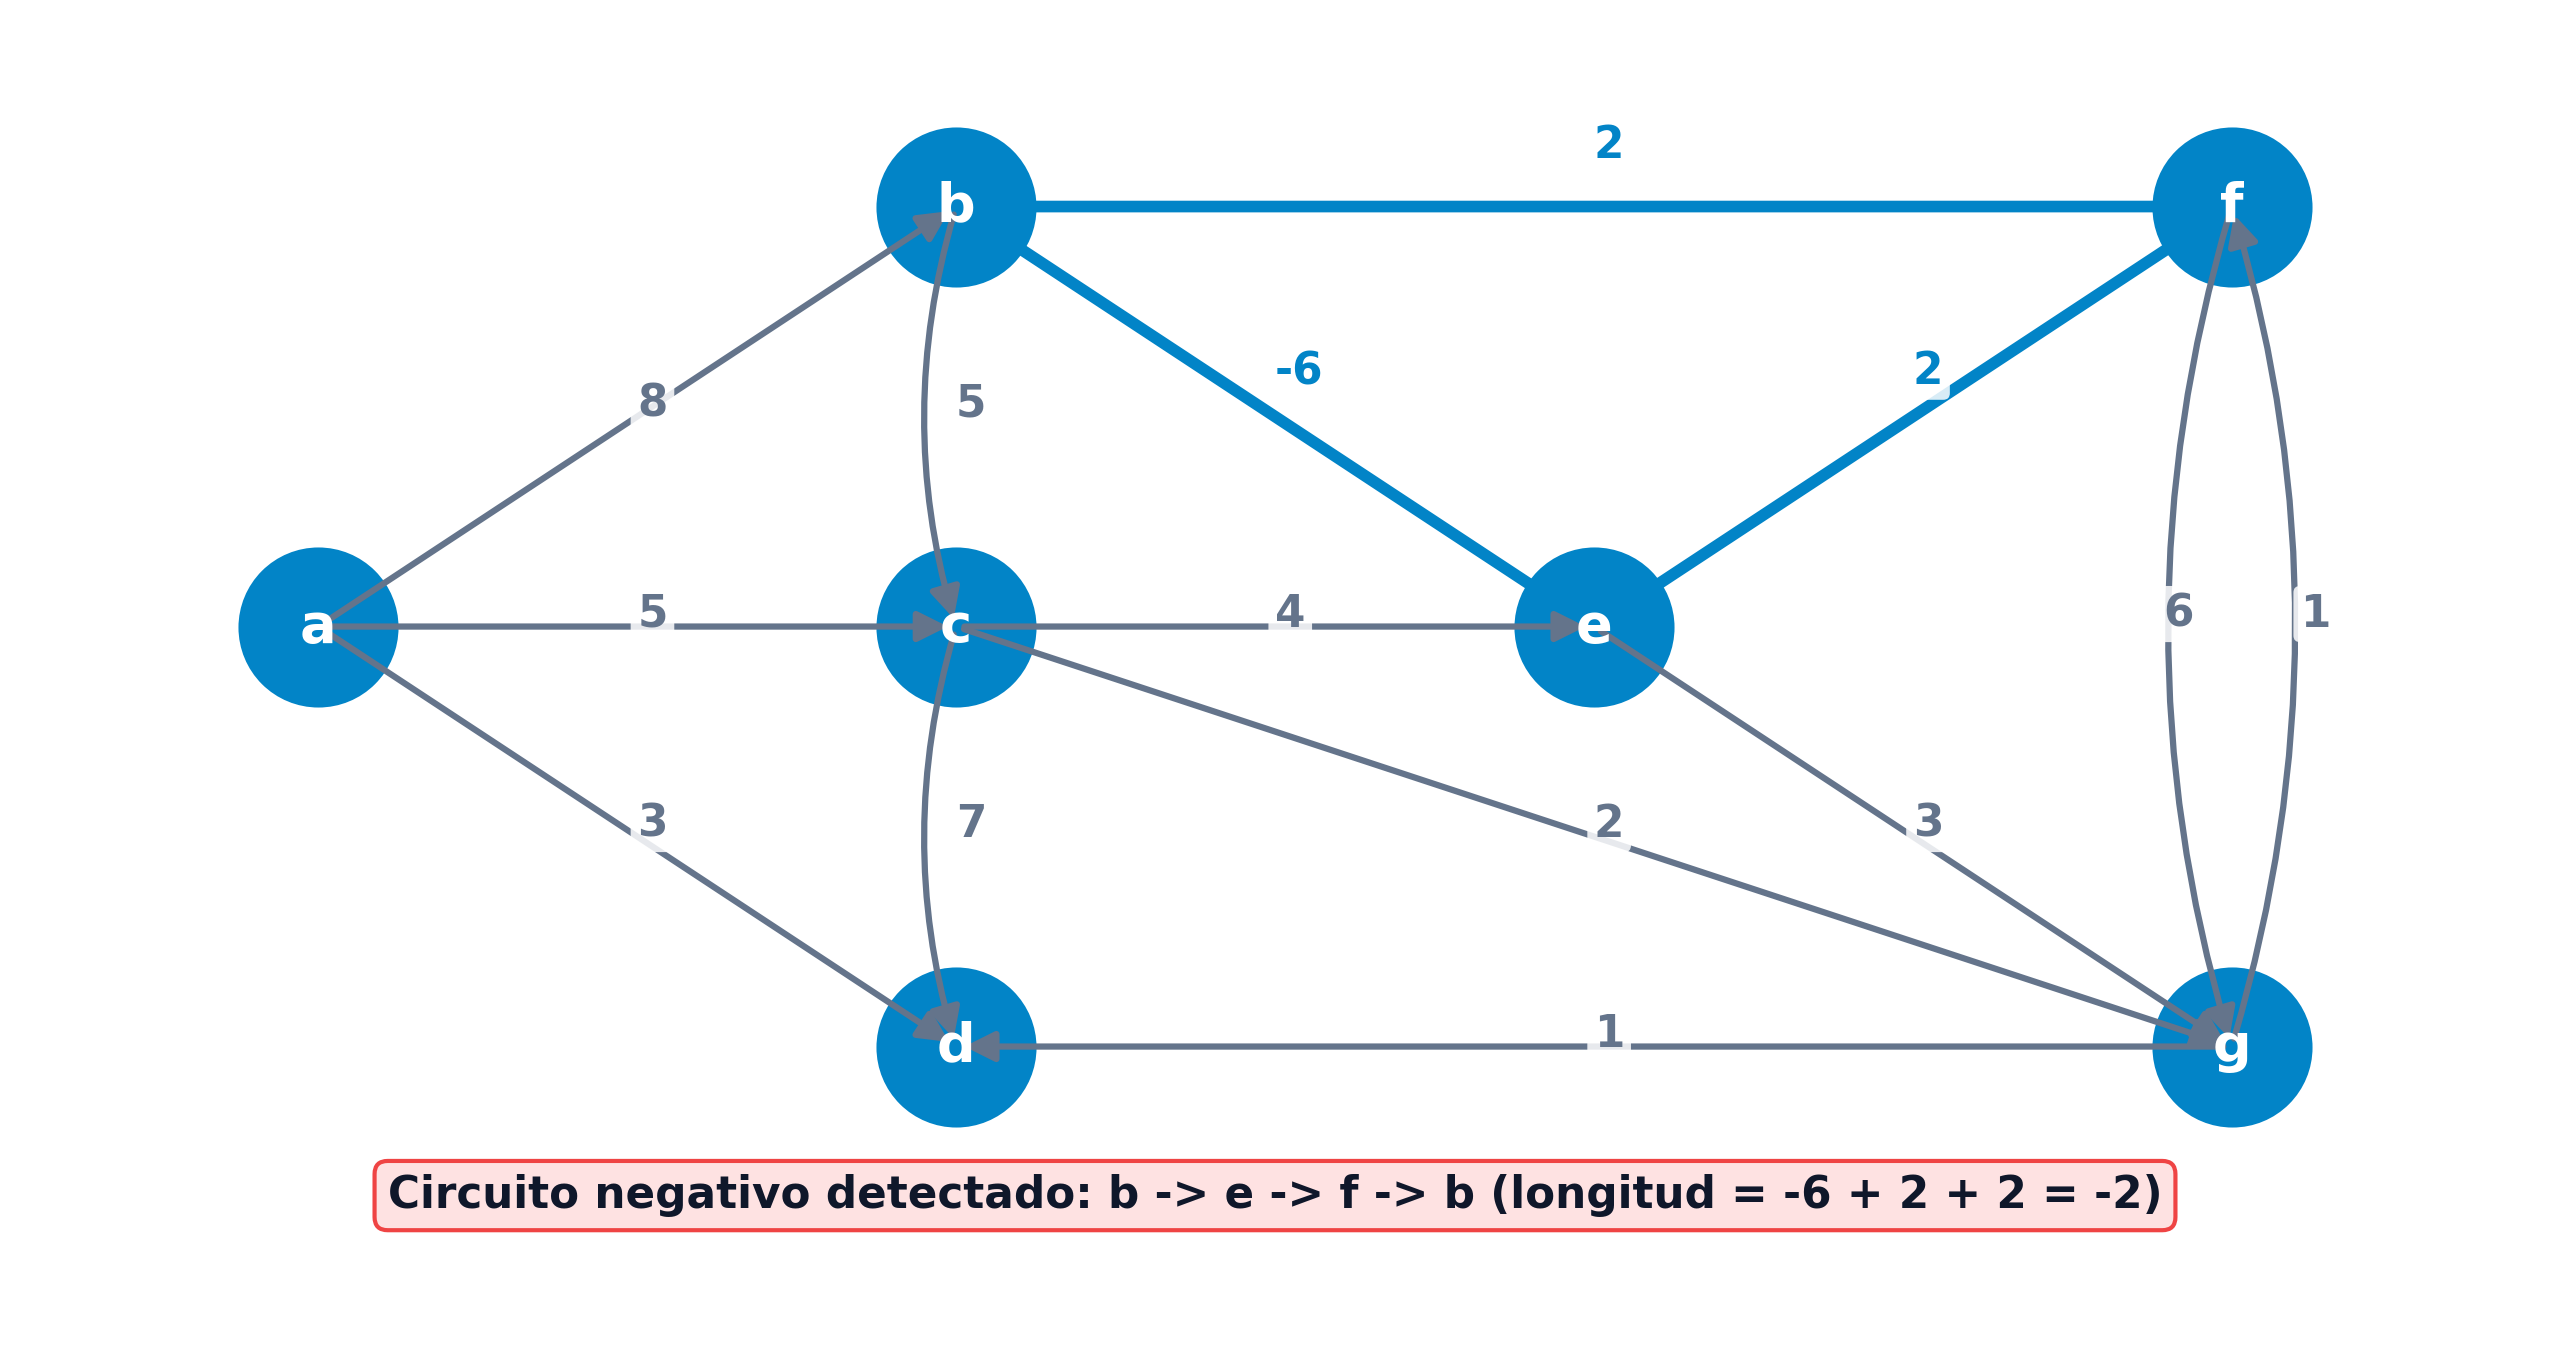
\includegraphics[width=0.95\linewidth,height=\textheight,keepaspectratio]{../images/bellman_ford_circuito_negativo_7nodos.png}
\end{center}
\end{column}

\begin{column}{0.55\linewidth}
\begin{itemize}
\item
  \textbf{Circuito negativo}: \(b \to e \to f \to b\) con coste
  acumulado \(-6 + 2 + 2 = -2 < 0\).
\item
  \textbf{Iteración \(m = 6\) (\(n-1\))}:
  \(u^6 = (0, 6, 5, 3, 0, 2, 3)\).
\item
  \textbf{Iteración suplementaria \(m = n = 7\)}:
  \(u_b^7 = \min \{ u_b^6, u_f^6 + 2 \} = \min \{ 6, 2+2 \} = 4\).
\item
  \textbf{Conclusión}:
  \(u_b^7 = 4 \neq 6 = u_b^6 \implies \mathbf{u}^7 \neq \mathbf{u}^6\).
  Demostrada formalmente la presencia del circuito negativo.
\end{itemize}
\end{column}
\end{columns}
\end{frame}

\section{Formulación en Programación Lineal
Primal-Dual}\label{formulaciuxf3n-en-programaciuxf3n-lineal-primal-dual}

\begin{frame}{Modelo Primal: Flujo de coste mínimo continuo}
\phantomsection\label{modelo-primal-flujo-de-coste-muxednimo-continuo}
\begin{itemize}
\item
  \textbf{Planteamiento}: Enviar 1 unidad de flujo desde el origen \(s\)
  al destino \(t\) al menor coste.
\item
  \textbf{Variables de decisión}: \(x_{ij} \in \{0, 1\}\) (1 si el arco
  \((i,j)\) forma parte del camino mínimo, 0 en otro caso).
\end{itemize}

\[
\begin{aligned}
\min_{\mathbf{x}} \quad & \sum_{(i,j) \in U} d_{ij} x_{ij} \\
\text{sujeto a} \quad & \sum_{k \mid (s,k) \in U} x_{sk} = 1 \quad (\text{Salida del nodo origen } s) \\
& \sum_{k \mid (k,t) \in U} x_{kt} = 1 \quad (\text{Entrada al nodo destino } t) \\
& \sum_{i \mid (i,k) \in U} x_{ik} = \sum_{j \mid (k,j) \in U} x_{kj}, \quad \forall k \neq s, t \quad (\text{Conservación de flujo}) \\
& x_{ij} \ge 0, \quad \forall (i, j) \in U
\end{aligned}
\]
\end{frame}

\begin{frame}{Teorema: Total Unimodularidad e Integridad (TUM)}
\phantomsection\label{teorema-total-unimodularidad-e-integridad-tum}
\begin{tcolorbox}[enhanced jigsaw, arc=.35mm, title=\textcolor{quarto-callout-important-color}{\faExclamation}\hspace{0.5em}{Total Unimodularidad de la matriz de incidencia}, titlerule=0mm, opacitybacktitle=0.6, left=2mm, rightrule=.15mm, colback=white, colframe=quarto-callout-important-color-frame, toprule=.15mm, opacityback=0, coltitle=black, breakable, colbacktitle=quarto-callout-important-color!10!white, bottomtitle=1mm, leftrule=.75mm, bottomrule=.15mm, toptitle=1mm]

La matriz de incidencia nodo-arco
\(\mathbf{A} \in \{-1, 0, 1\}^{n \times m}\) de cualquier digrafo es
\textbf{totalmente unimodular} (TUM).

Puesto que el vector de balances nodales
\(\mathbf{b} = (1, 0, \dots, 0, -1)^T\) es entero, todas las soluciones
básicas del poliedro continuo son \textbf{estrictamente enteras}:

\[x_{ij}^* \in \{0, 1\}\]

\end{tcolorbox}

\begin{itemize}
\tightlist
\item
  \textbf{Garantía matemática}: La relajación continua de PL resuelve
  exactamente el problema combinatorio discreto sin necesitar
  restricciones de programación entera.
\end{itemize}
\end{frame}

\begin{frame}{Modelo Dual: Potenciales nodales}
\phantomsection\label{modelo-dual-potenciales-nodales}
\begin{itemize}
\tightlist
\item
  \textbf{Variables duales \(u_i \in \mathbb{R}\) asociadas a la
  ecuación de balance de cada nodo \(i \in V\)}:
\end{itemize}

\[
\begin{aligned}
\max_{\mathbf{u}} \quad & u_t - u_s \\
\text{sujeto a} \quad & u_j - u_i \le d_{ij}, \quad \forall (i, j) \in U \\
& u_i \in \mathbb{R}, \quad \forall i \in V
\end{aligned}
\]

\begin{itemize}
\tightlist
\item
  \textbf{Fijación de Referencia y Distancia Óptima}: Al fijar el origen
  en \(u_s = 0\), la variable dual óptima \(u_j^*\) coincide exactamente
  con la \textbf{distancia mínima \(d(s, j)\)} desde \(s\) hasta \(j\).
\end{itemize}
\end{frame}

\begin{frame}{Holgura complementaria e interpretación geométrica}
\phantomsection\label{holgura-complementaria-e-interpretaciuxf3n-geomuxe9trica}
\begin{itemize}
\item
  \textbf{Condiciones de Holgura Complementaria KKT}:
  \[x_{ij}^* \left( d_{ij} - (u_j^* - u_i^*) \right) = 0, \quad \forall (i, j) \in U\]
\item
  \textbf{Significado geométrico de la dualidad}:

  \begin{itemize}
  \tightlist
  \item
    \textbf{Arco en la ruta óptima (\(x_{ij}^* = 1\))}: La restricción
    dual se satisface con \textbf{igualdad estricta}:
    \(u_j^* - u_i^* = d_{ij}\).
  \item
    \textbf{Arco no utilizado (\(x_{ij}^* = 0\))}: La diferencia de
    potencial entre extremos no supera la distancia directa:
    \(u_j^* - u_i^* < d_{ij}\).
  \end{itemize}
\end{itemize}
\end{frame}

\begin{frame}{Ejemplo: Formulación primal completa (7 nodos)}
\phantomsection\label{ejemplo-formulaciuxf3n-primal-completa-7-nodos}
\begin{columns}[T]
\begin{column}{0.45\linewidth}
\begin{center}
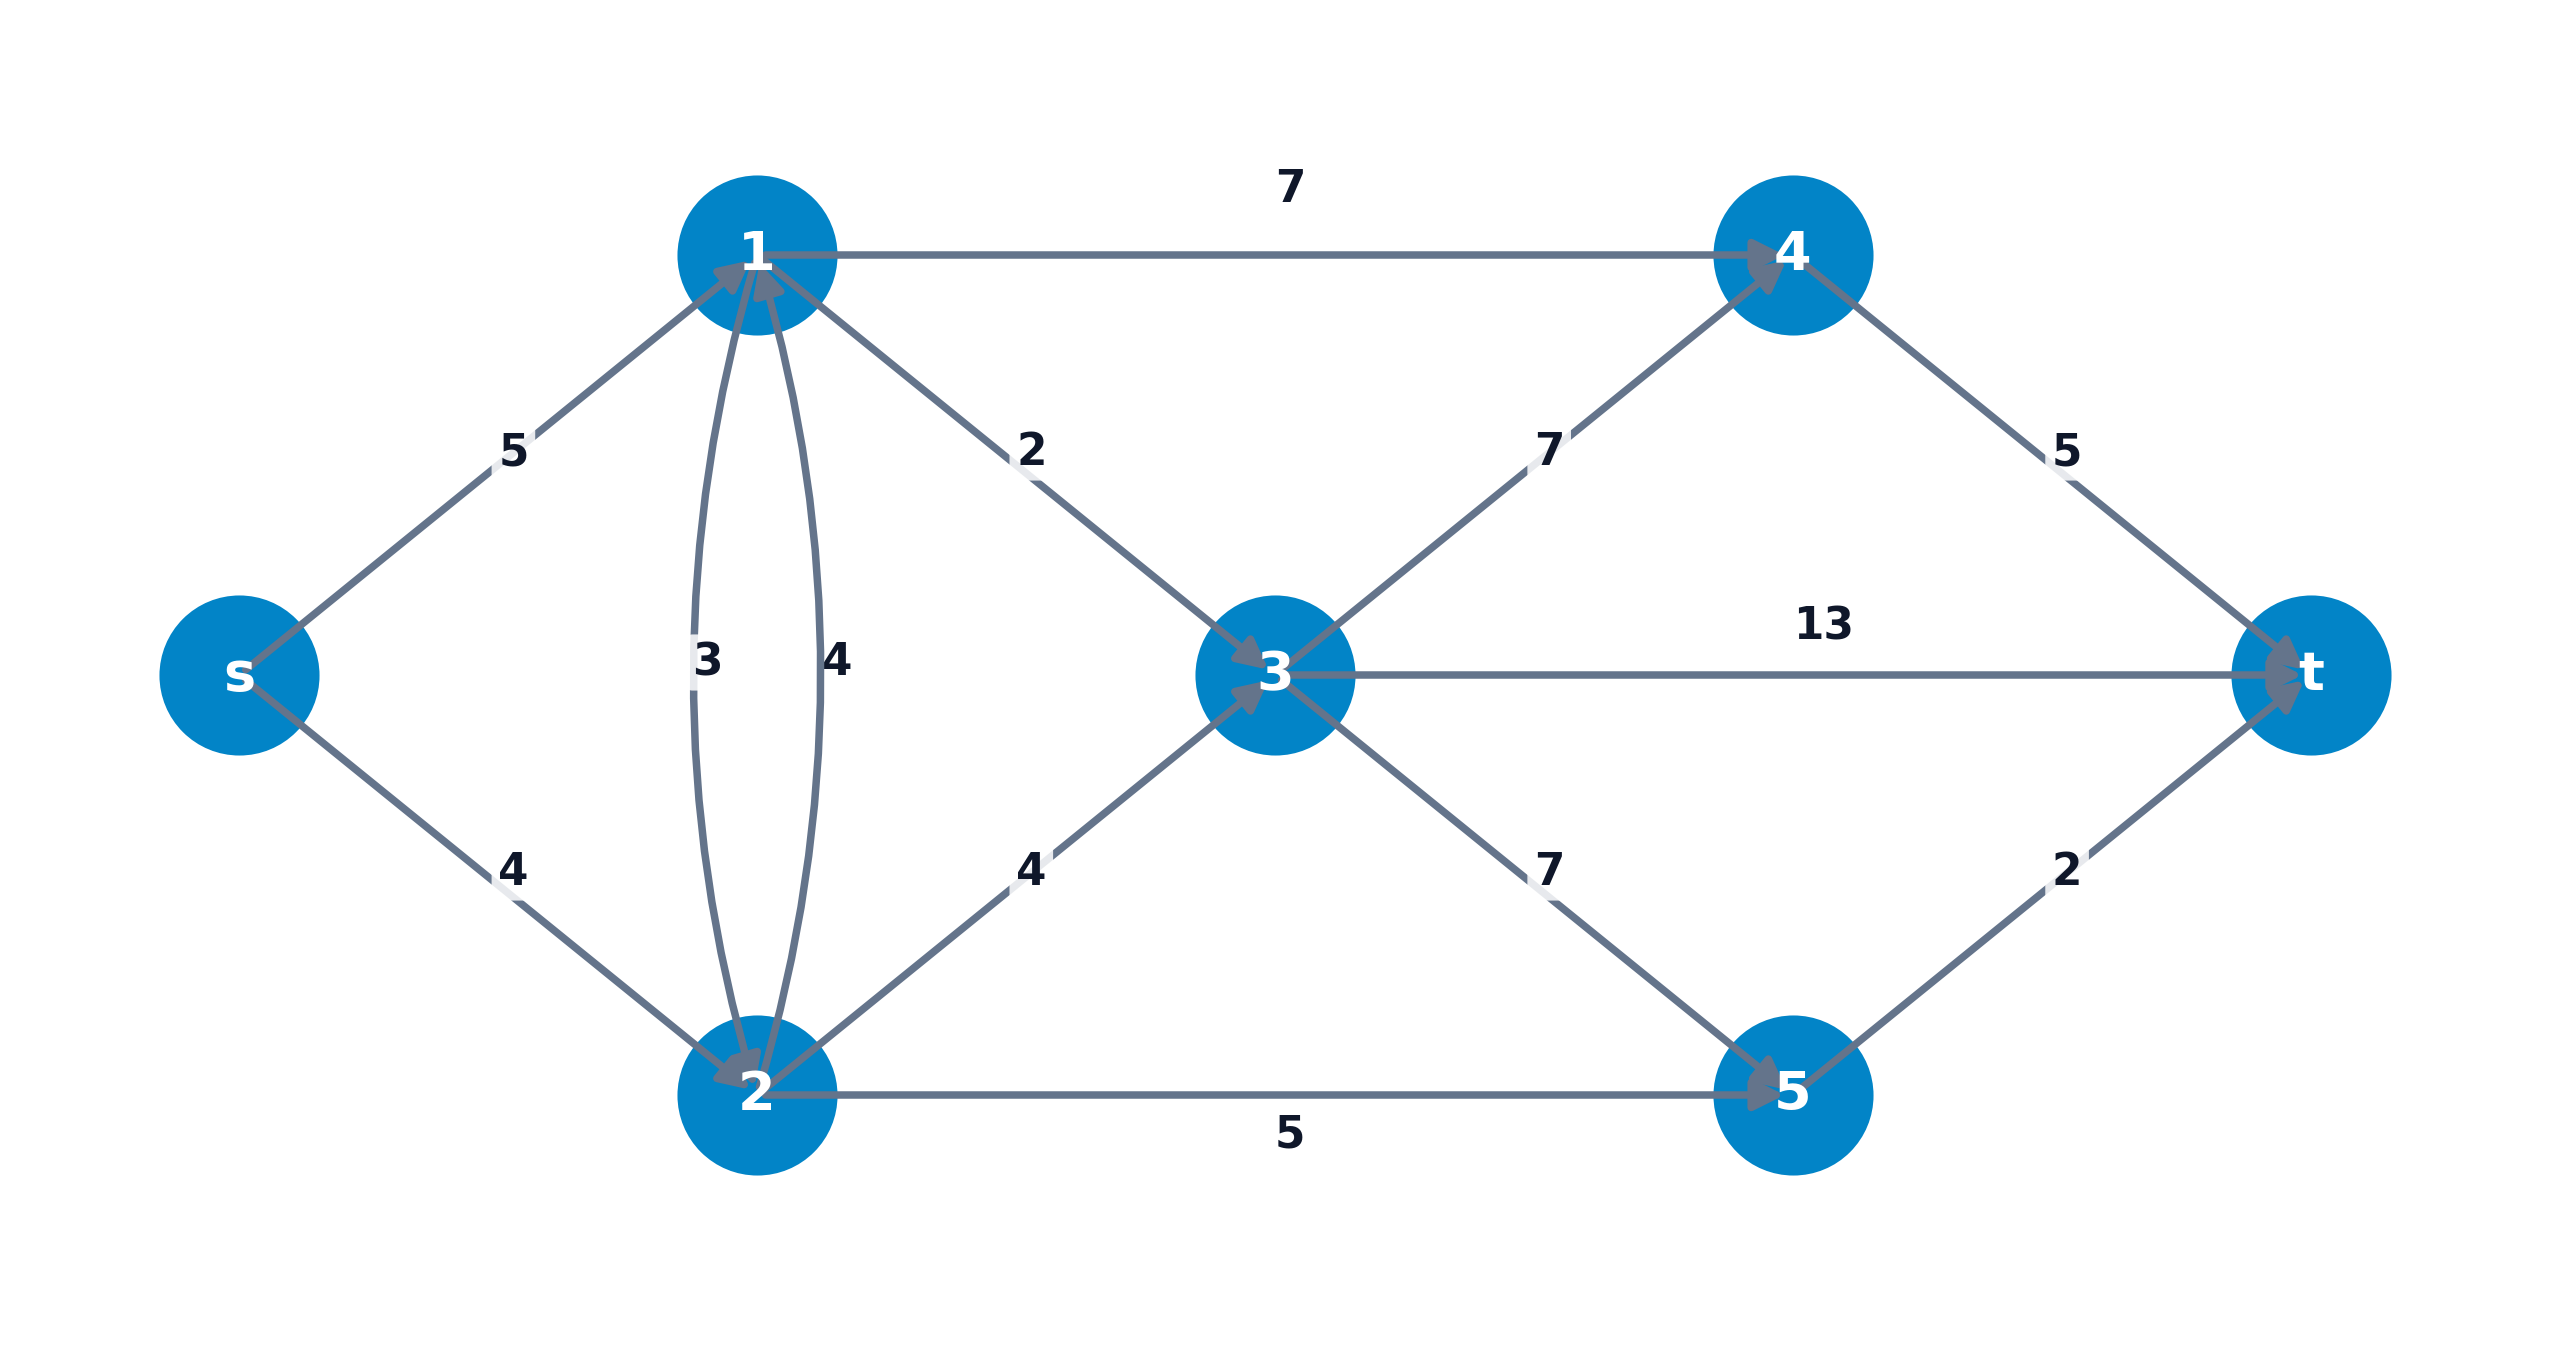
\includegraphics[width=0.95\linewidth,height=\textheight,keepaspectratio]{../images/linear_programming_ejemplo_7nodos.png}
\end{center}
\end{column}

\begin{column}{0.55\linewidth}
\begin{itemize}
\item
  \textbf{Función Objetivo}: \[ \small
  \begin{aligned}
  \min z = \ & 5 x_{s1} + 4 x_{s2} + 4 x_{12} + 2 x_{13} + 7 x_{14} + 3 x_{21} \\
  & + 4 x_{23} + 5 x_{25} + 7 x_{34} + 7 x_{35} + 13 x_{3t} \\
  & + 5 x_{4t} + 2 x_{5t}
  \end{aligned}
  \]
\item
  \textbf{Restricción Origen (\(s\))}: \(x_{s1} + x_{s2} = 1\)
\item
  \textbf{Restricción Destino (\(t\))}: \(x_{3t} + x_{4t} + x_{5t} = 1\)
\end{itemize}
\end{column}
\end{columns}
\end{frame}

\begin{frame}{Ejemplo: Formulación primal completa (cont.)}
\phantomsection\label{ejemplo-formulaciuxf3n-primal-completa-cont.}
\begin{columns}[T]
\begin{column}{0.45\linewidth}
\begin{center}
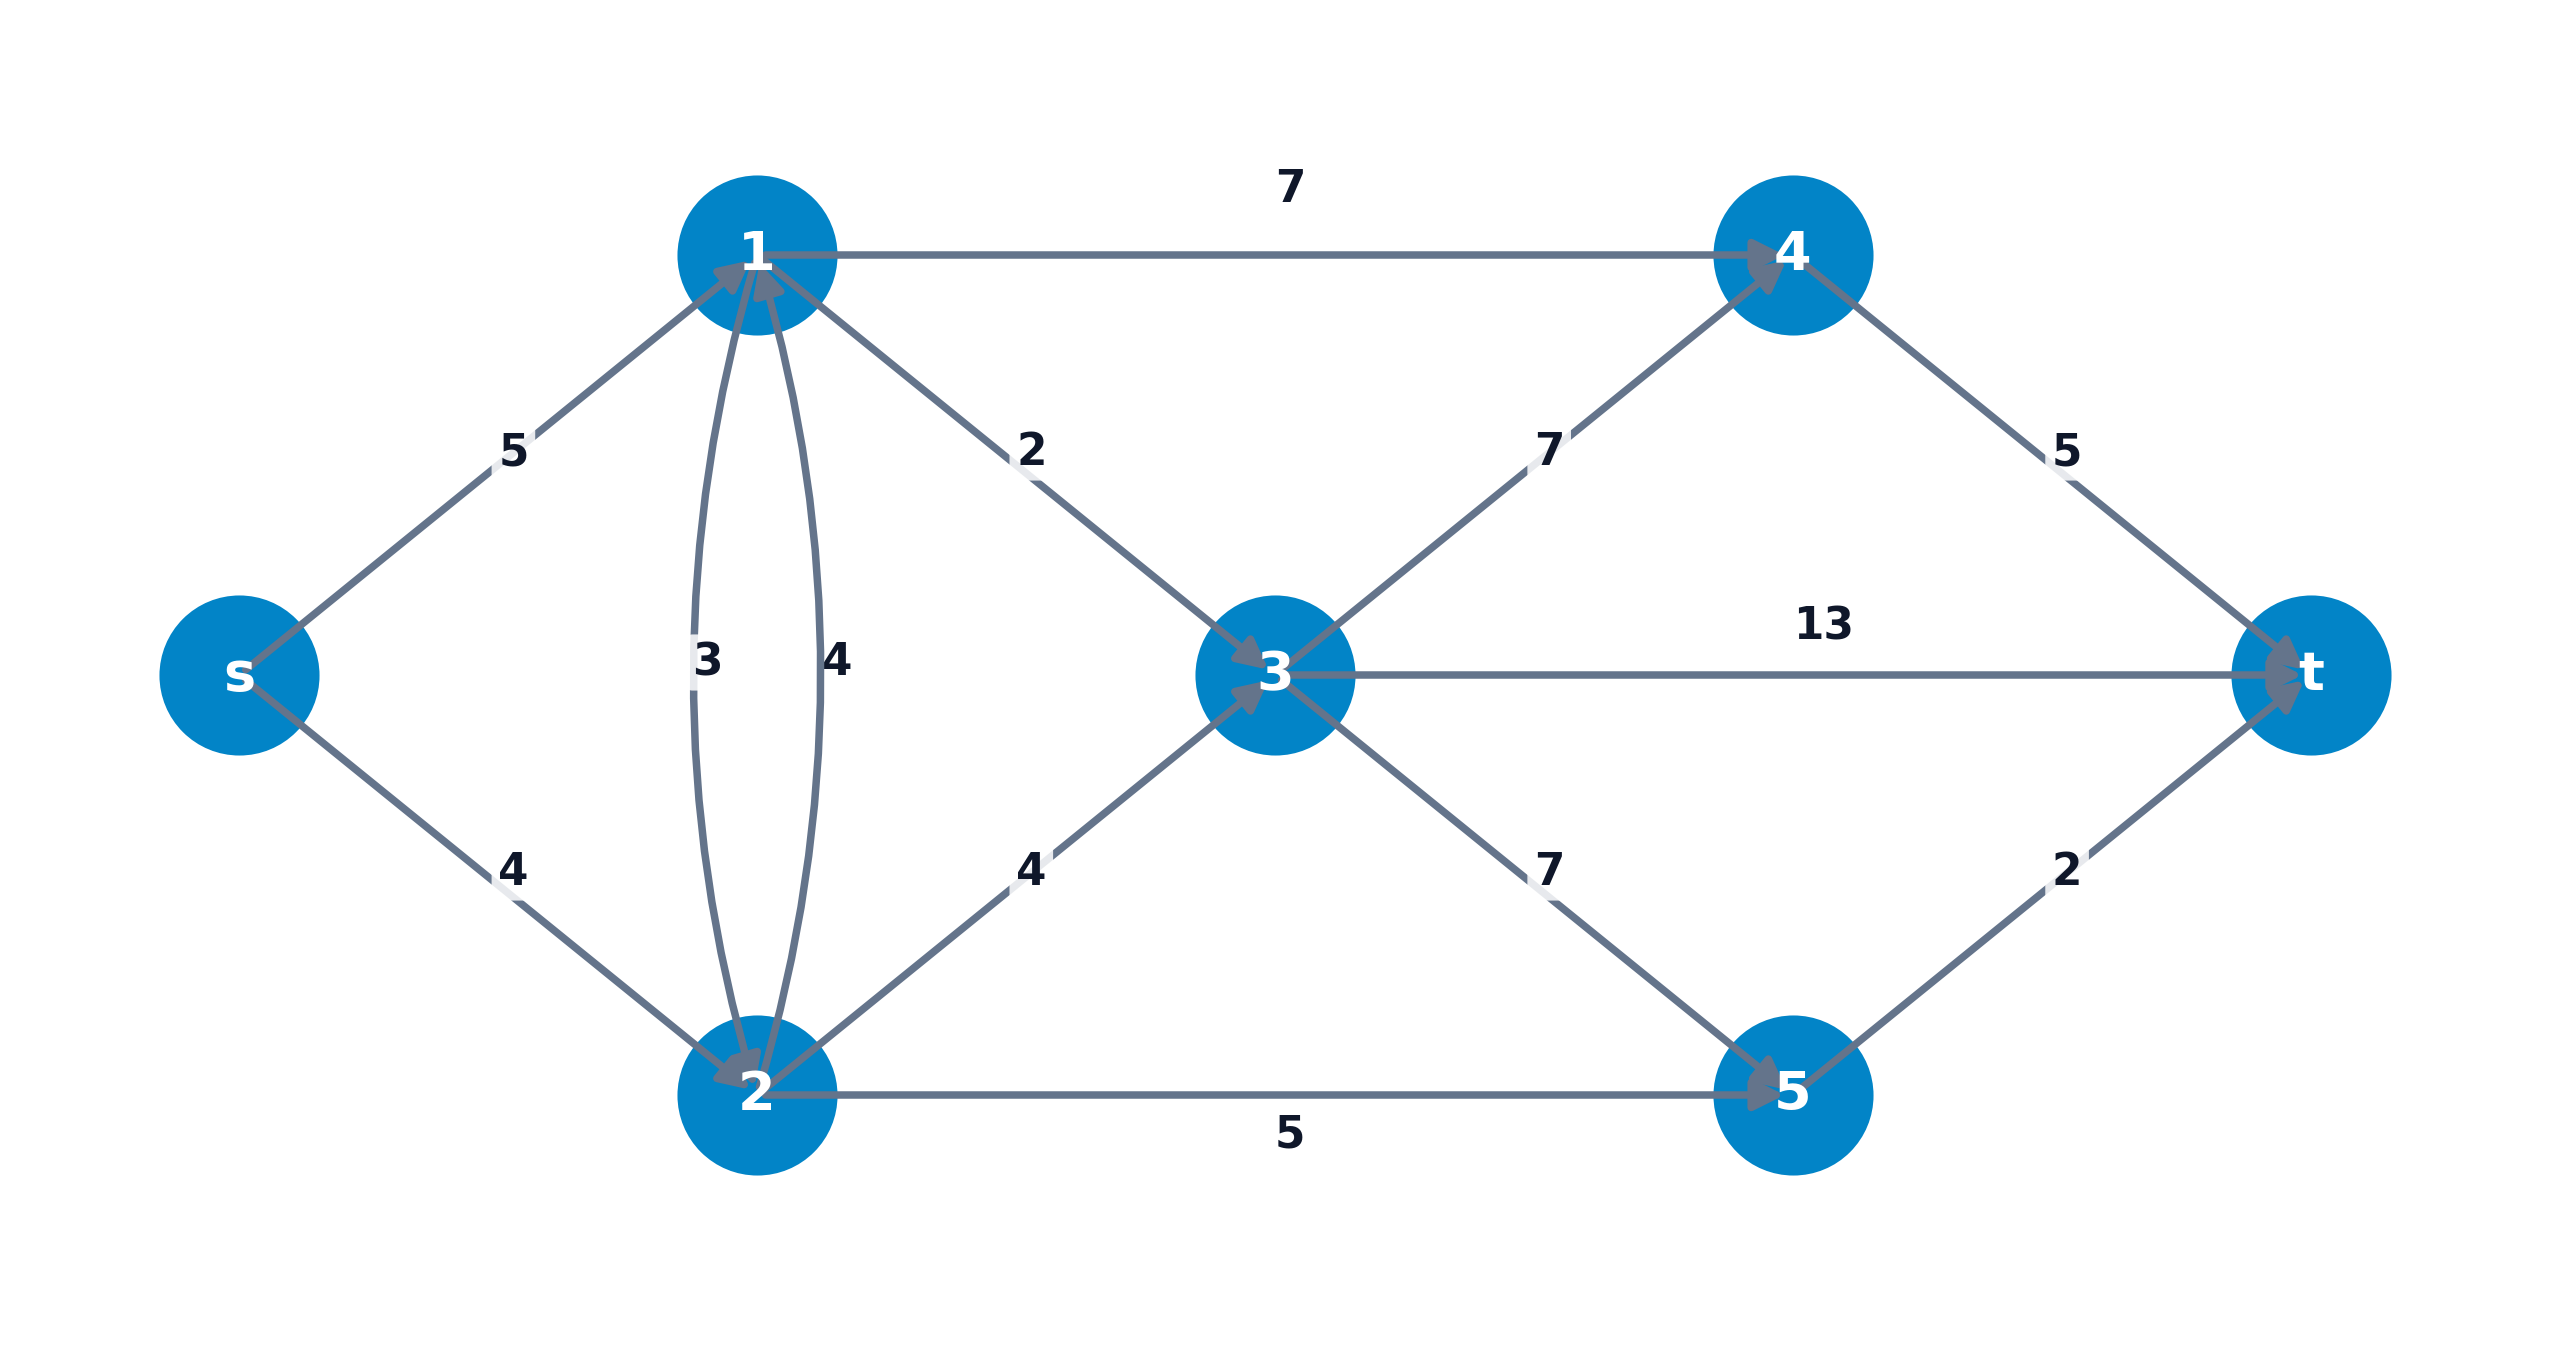
\includegraphics[width=0.95\linewidth,height=\textheight,keepaspectratio]{../images/linear_programming_ejemplo_7nodos.png}
\end{center}
\end{column}

\begin{column}{0.55\linewidth}
\begin{itemize}
\item
  \textbf{Conservación de flujo en nodos intermedios}: \[ \small
  \begin{aligned}
  \text{Nodo 1:} \quad & x_{s1} + x_{21} = x_{12} + x_{13} + x_{14} \\
  \text{Nodo 2:} \quad & x_{s2} + x_{12} = x_{21} + x_{23} + x_{25} \\
  \text{Nodo 3:} \quad & x_{13} + x_{23} = x_{34} + x_{35} + x_{3t} \\
  \text{Nodo 4:} \quad & x_{14} + x_{34} = x_{4t} \\
  \text{Nodo 5:} \quad & x_{25} + x_{35} = x_{5t}
  \end{aligned}
  \]
\item
  \textbf{Naturaleza de las variables}:
  \[x_{ij} \in \{0, 1\}, \quad \forall (i, j) \in U\]
\end{itemize}
\end{column}
\end{columns}
\end{frame}

\section{Caminos mínimos entre todos los pares de
nodos}\label{caminos-muxednimos-entre-todos-los-pares-de-nodos}

\begin{frame}{Motivación y estrategia global}
\phantomsection\label{motivaciuxf3n-y-estrategia-global}
\begin{itemize}
\item
  \textbf{Necesidad práctica}: Determinar las distancias mínimas entre
  \textbf{todos los pares de vértices \((i, j) \in V \times V\)}.
\item
  \textbf{Aproximaciones preliminares}:

  \begin{itemize}
  \tightlist
  \item
    Repetir \(n\) veces un algoritmo de origen único (Dijkstra o
    Bellman-Ford).
  \item
    Con Dijkstra (\(d_{ij} \ge 0\)):
    \(n \times O(m + n \log n) = O(nm + n^2 \log n)\).
  \item
    Con Bellman-Ford: \(n \times O(n^3) = O(n^4)\).
  \end{itemize}
\item
  \textbf{Desaprovechamiento de información}: La resolución
  independiente no reutiliza la información de subcaminos compartidos.
\end{itemize}
\end{frame}

\begin{frame}{Álgebra Min-Suma o Tropical (Definición y Operador)}
\phantomsection\label{uxe1lgebra-min-suma-o-tropical-definiciuxf3n-y-operador}
\begin{tcolorbox}[enhanced jigsaw, arc=.35mm, title=\textcolor{quarto-callout-note-color}{\faInfo}\hspace{0.5em}{Producto matricial Min-Suma}, titlerule=0mm, opacitybacktitle=0.6, left=2mm, rightrule=.15mm, colback=white, colframe=quarto-callout-note-color-frame, toprule=.15mm, opacityback=0, coltitle=black, breakable, colbacktitle=quarto-callout-note-color!10!white, bottomtitle=1mm, leftrule=.75mm, bottomrule=.15mm, toptitle=1mm]

Dadas dos matrices \(A, B \in \overline{\mathbb{R}}^{n \times n}\), se
define el \textbf{producto matricial Min-Suma} \(C = A \otimes B\) en el
semianillo \((\mathbb{R} \cup \{\infty\}, \min, +)\) mediante la
sustitución operatoria \(\sum \to \min\) y \(\cdot \to +\):

\[ \small
\begin{aligned}
\text{Producto Estándar: } & c_{ij} = \sum_{k=1}^n a_{ik} \cdot b_{kj} \\
\implies \quad \text{Producto Min-Suma: } & c_{ij} = \min_{1 \le k \le n} \left\{ a_{ik} + b_{kj} \right\}
\end{aligned}
\]

\end{tcolorbox}

\begin{itemize}
\tightlist
\item
  \textbf{Matriz Inicial \(D^{(1)} = D\)}:
  \[d_{ij}^{(1)} = d_{ij} \quad (\text{distancias directas de los arcos})\]
\end{itemize}
\end{frame}

\begin{frame}{Potencias Matriciales \(D^m\) y Paralelismo con
Bellman-Ford}
\phantomsection\label{potencias-matriciales-dm-y-paralelismo-con-bellman-ford}
\begin{columns}[T]
\begin{column}{0.52\linewidth}
\begin{tcolorbox}[enhanced jigsaw, arc=.35mm, title=\textcolor{quarto-callout-note-color}{\faInfo}\hspace{0.5em}{Relación de recurrencia en álgebra Min-Suma}, titlerule=0mm, opacitybacktitle=0.6, left=2mm, rightrule=.15mm, colback=white, colframe=quarto-callout-note-color-frame, toprule=.15mm, opacityback=0, coltitle=black, breakable, colbacktitle=quarto-callout-note-color!10!white, bottomtitle=1mm, leftrule=.75mm, bottomrule=.15mm, toptitle=1mm]

La componente \((d_{ij})^m\) de \(D^m = D^{m-1} \otimes D\) contiene la
\textbf{distancia mínima entre \(i\) y \(j\) en a lo sumo \(m\) arcos}:

\[ \small
\begin{aligned}
(d_{ij})^{m} = \min \Big\{ & (d_{ij})^{m-1}, \\
& \min_{k \in V} \{ (d_{ik})^{m-1} + d_{kj} \} \Big\}
\end{aligned}
\]

\end{tcolorbox}
\end{column}

\begin{column}{0.48\linewidth}
\begin{itemize}
\tightlist
\item
  \textbf{Equivalencia Didáctica con Bellman-Ford}:

  \begin{itemize}
  \tightlist
  \item
    La fila \(i\)-ésima de la matriz \(D^m\) equivale exactamente a
    resolver la iteración \(m\) de Bellman-Ford con el \textbf{vértice
    \(i\) como origen}.
  \item
    El cálculo \(D^m\) resuelve en paralelo el problema para los
    \textbf{\(n\) posibles nodos origen} de la red.
  \end{itemize}
\end{itemize}
\end{column}
\end{columns}
\end{frame}

\begin{frame}{Convergencia y Exponenciación Binaria (\emph{Repeated
Squaring})}
\phantomsection\label{convergencia-y-exponenciaciuxf3n-binaria-repeated-squaring}
\begin{columns}[T]
\begin{column}{0.5\linewidth}
\begin{itemize}
\tightlist
\item
  \textbf{Convergencia y Complejidad Secuencial}:

  \begin{itemize}
  \tightlist
  \item
    \textbf{Cota de finitud en \(D^{n-1}\)}: Cualquier camino simple en
    una red de \(n\) vértices contiene a lo sumo \(n-1\) arcos.
  \item
    \textbf{Convergencia}: Sin circuitos de coste negativo, el algoritmo
    converge en \(D^{n-1}\).
  \item
    \textbf{Complejidad Secuencial}: \(n-1\) productos matriciales
    \(\implies \mathbf{O(n^4)}\).
  \end{itemize}
\end{itemize}
\end{column}

\begin{column}{0.5\linewidth}
\begin{itemize}
\tightlist
\item
  \textbf{Optimización por Exponenciación Binaria}:

  \begin{itemize}
  \tightlist
  \item
    Evaluamos potencias cuadráticas:
    \[ \small D^1 \to D^2 \to D^4 \to D^8 \dots \to D^{2^{\lceil \log_2(n-1) \rceil}} \]
  \item
    \textbf{Complejidad Optimizada}: Se realizan únicamente
    \(\lceil \log_2(n-1) \rceil\) productos
    \(\implies \mathbf{O(n^3 \log n)}\).
  \end{itemize}
\end{itemize}
\end{column}
\end{columns}
\end{frame}

\begin{frame}{Ejemplo: Multiplicación de matrices min-suma --- Matriz
D\^{}(1)}
\phantomsection\label{ejemplo-multiplicaciuxf3n-de-matrices-min-suma-matriz-d1}
\begin{columns}[T]
\begin{column}{0.42\linewidth}
\begin{center}
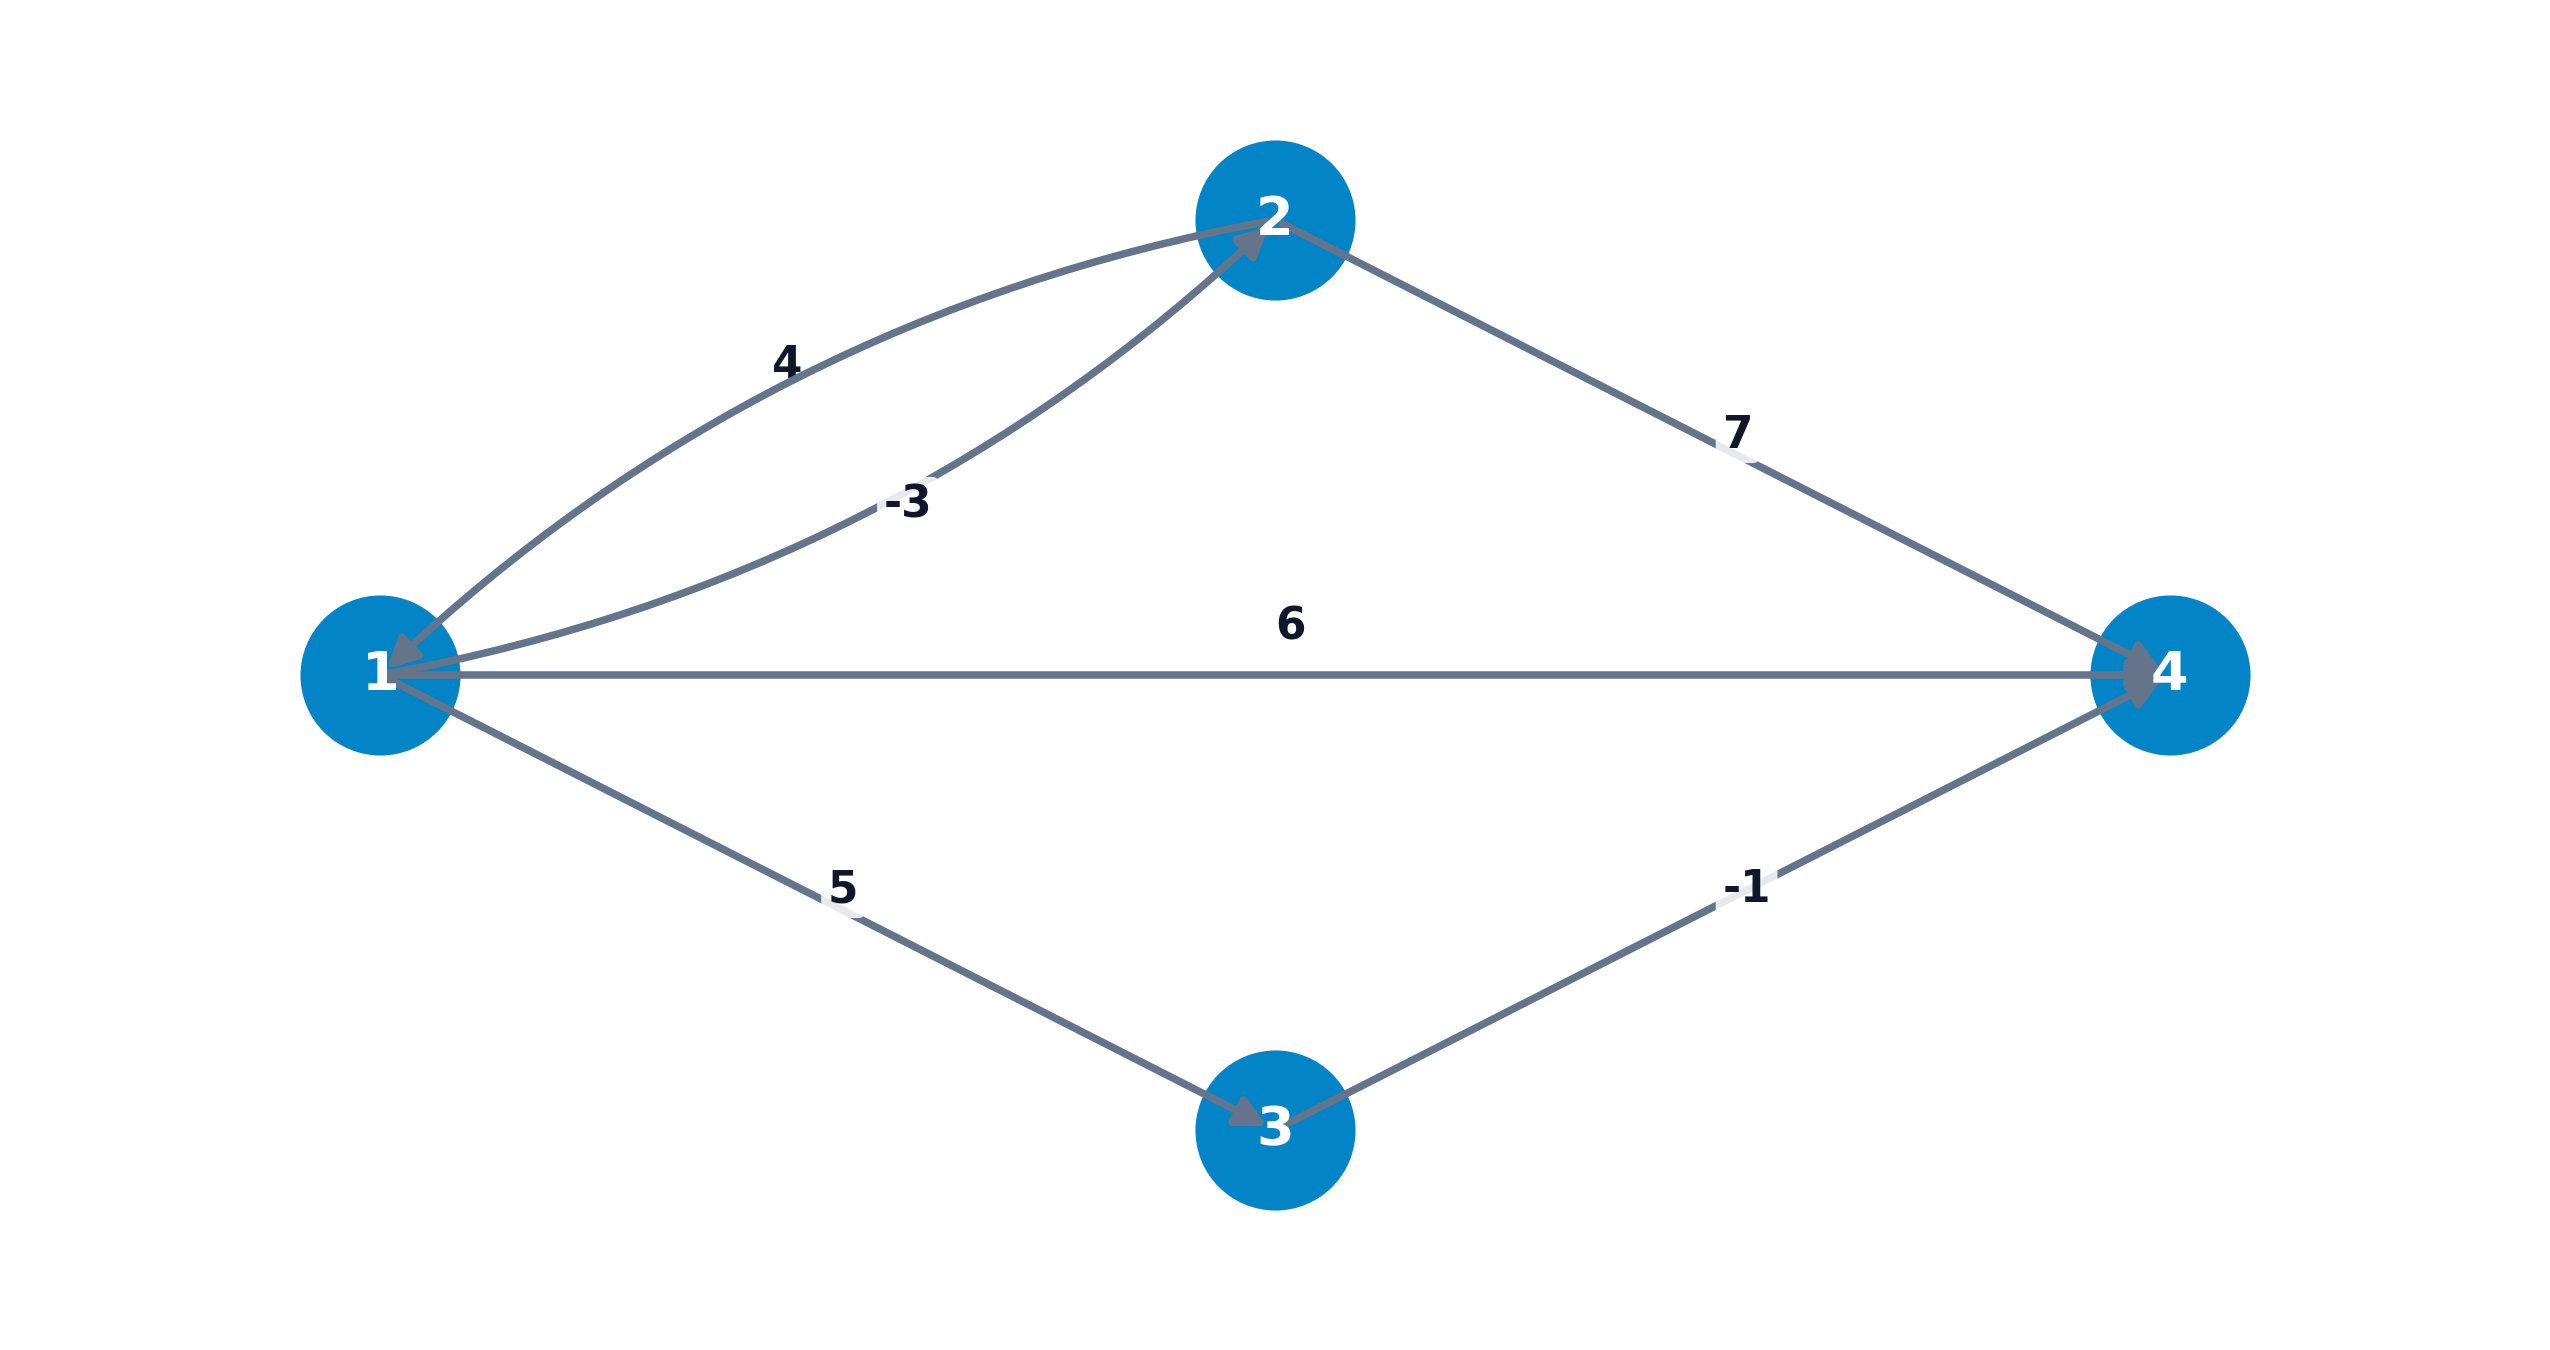
\includegraphics[width=0.95\linewidth,height=\textheight,keepaspectratio]{../images/matrix_multiplication_ejemplo_4nodos.png}
\end{center}
\end{column}

\begin{column}{0.58\linewidth}
\begin{itemize}
\item
  \textbf{Matriz Inicial de Distancias Directas \(D^{(1)}\)}: \[ \small
  D^{(1)} = \begin{pmatrix}
  0 & 4 & 5 & 6 \\
  -3 & 0 & \infty & 7 \\
  \infty & \infty & 0 & -1 \\
  \infty & \infty & \infty & 0
  \end{pmatrix}
  \]
\item
  Contiene las distancias directas entre todo par de vértices
  \(i, j \in V\) (caminos de a lo sumo 1 arco).
\end{itemize}
\end{column}
\end{columns}
\end{frame}

\begin{frame}{Ejemplo: Multiplicación de matrices min-suma --- Matriz
D\^{}(2)}
\phantomsection\label{ejemplo-multiplicaciuxf3n-de-matrices-min-suma-matriz-d2}
\begin{columns}[T]
\begin{column}{0.42\linewidth}
\begin{center}
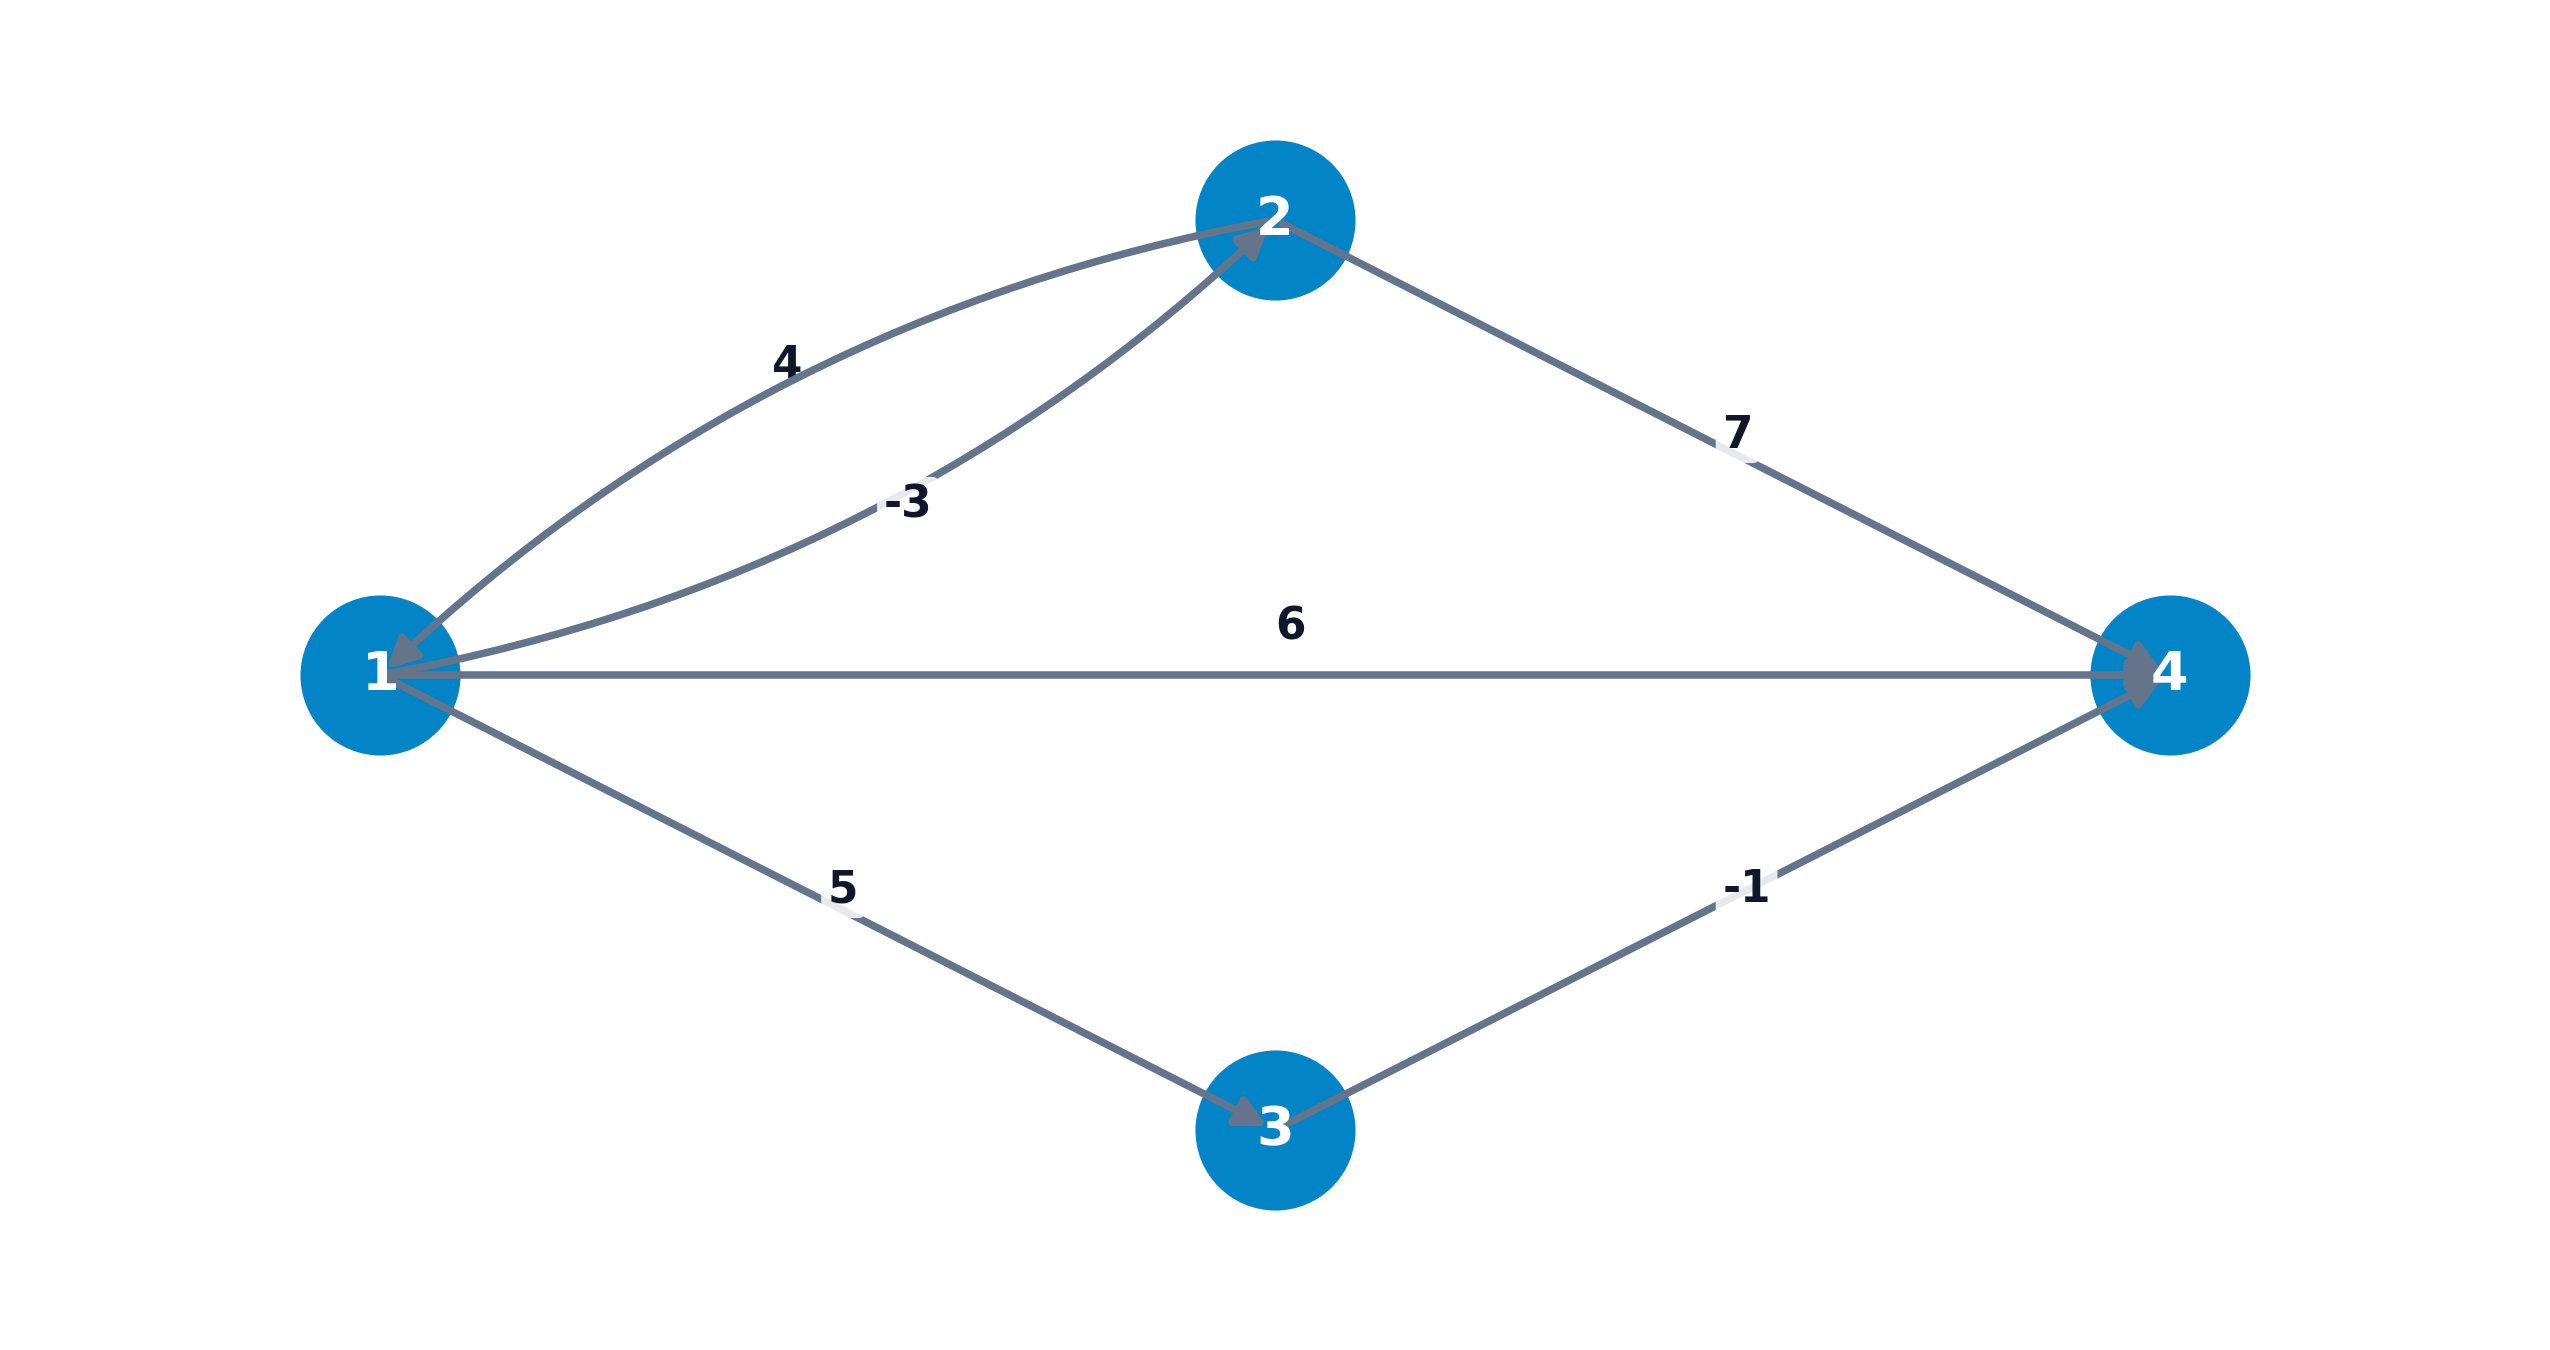
\includegraphics[width=0.95\linewidth,height=\textheight,keepaspectratio]{../images/matrix_multiplication_ejemplo_4nodos.png}
\end{center}
\end{column}

\begin{column}{0.58\linewidth}
\begin{itemize}
\item
  \textbf{Iteración 2 (\(D^{(2)} = D^{(1)} \otimes D^{(1)}\) - 2 arcos o
  menos)}: \[ \small
  D^{(2)} = \begin{pmatrix}
  0 & 4 & 5 & \textcolor{forestgreen}{\mathbf{4}} \\
  -3 & 0 & \textcolor{forestgreen}{\mathbf{2}} & \textcolor{forestgreen}{\mathbf{3}} \\
  \infty & \infty & 0 & -1 \\
  \infty & \infty & \infty & 0
  \end{pmatrix}
  \]
\item
  \textbf{Relajaciones destacadas}:

  \begin{itemize}
  \tightlist
  \item
    \((d_{14})^2 = \min \{ 6, \ 5 + (-1) \} = \textcolor{forestgreen}{\mathbf{4}}\)
    (vía \(1 \to 3 \to 4\)).
  \item
    \((d_{23})^2 = \min \{ \infty, \ -3 + 5 \} = \textcolor{forestgreen}{\mathbf{2}}\)
    (vía \(2 \to 1 \to 3\)).
  \end{itemize}
\end{itemize}
\end{column}
\end{columns}
\end{frame}

\begin{frame}{Ejemplo: Multiplicación de matrices min-suma --- Matriz
D\^{}(3)}
\phantomsection\label{ejemplo-multiplicaciuxf3n-de-matrices-min-suma-matriz-d3}
\begin{columns}[T]
\begin{column}{0.42\linewidth}
\begin{center}
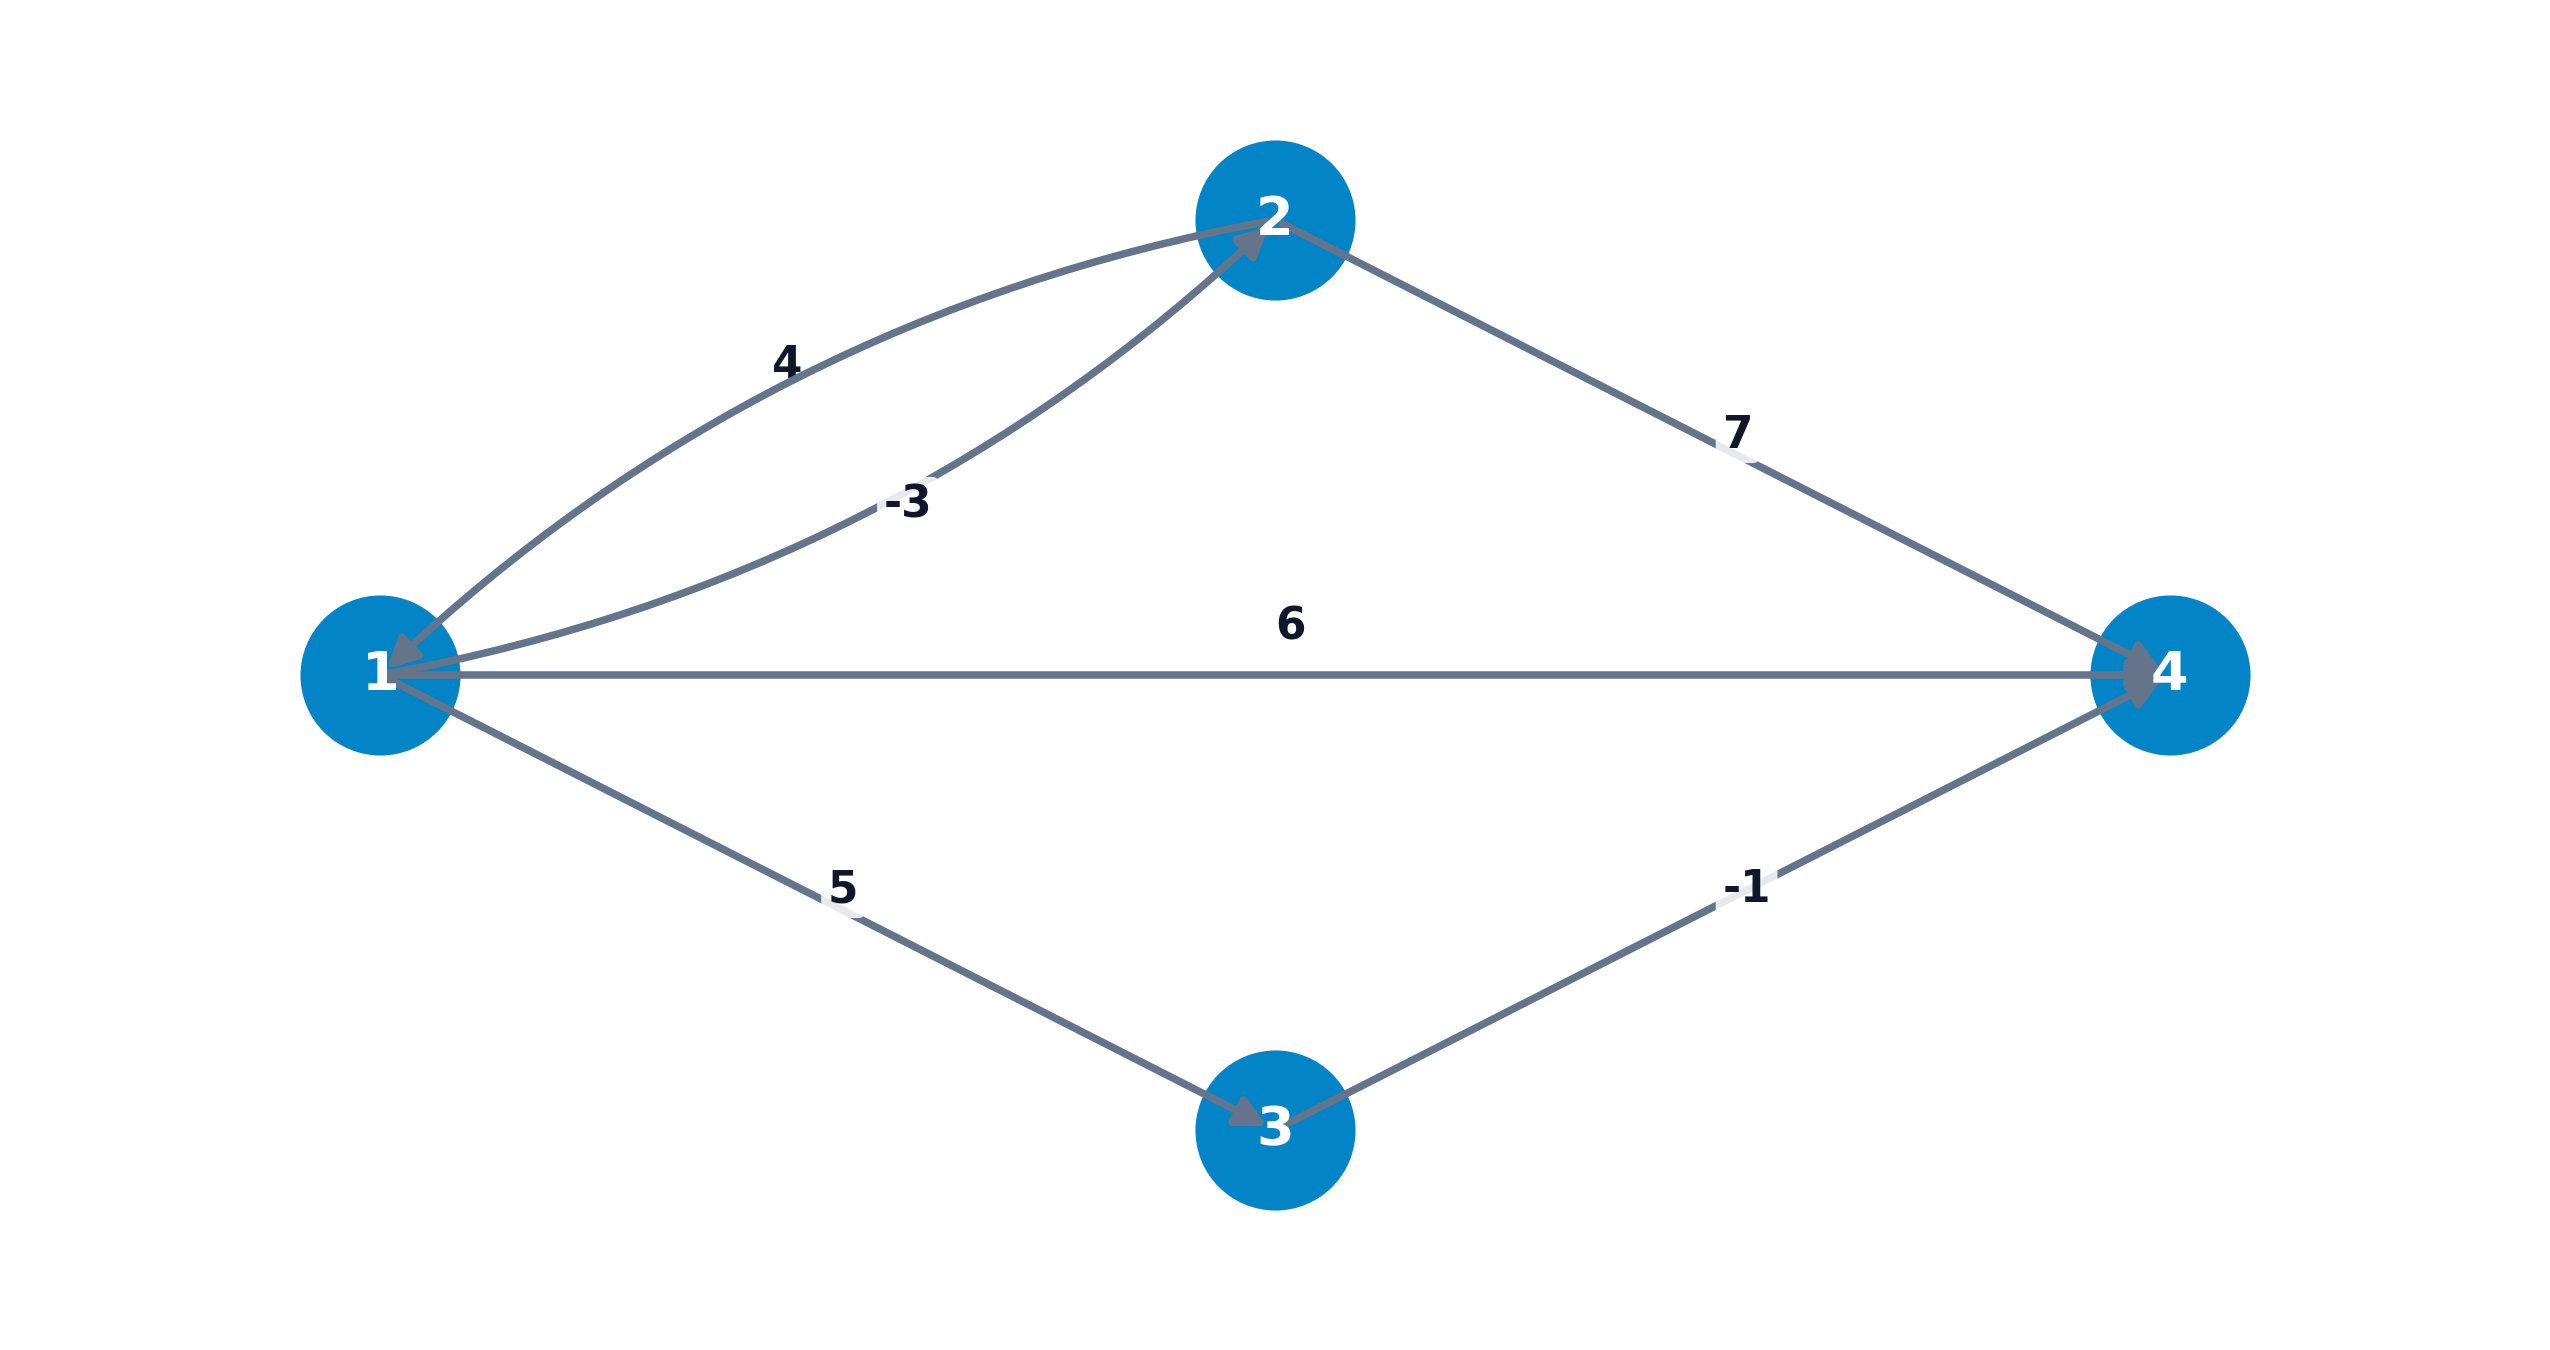
\includegraphics[width=0.95\linewidth,height=\textheight,keepaspectratio]{../images/matrix_multiplication_ejemplo_4nodos.png}
\end{center}
\end{column}

\begin{column}{0.58\linewidth}
\begin{itemize}
\item
  \textbf{Iteración 3 (\(D^{(3)} = D^{(2)} \otimes D^{(1)}\) - 3 arcos o
  menos)}: \[ \small
  D^{(3)} = \begin{pmatrix}
  0 & 4 & 5 & 4 \\
  -3 & 0 & 2 & \textcolor{forestgreen}{\mathbf{1}} \\
  \infty & \infty & 0 & -1 \\
  \infty & \infty & \infty & 0
  \end{pmatrix}
  \]
\item
  \textbf{Relajación de \((d_{24})^3\)}:
  \(\min \{ 3, \ -3 + 4 \} = \textcolor{forestgreen}{\mathbf{1}}\) (vía
  \(2 \to 1 \to 3 \to 4\)).
\item
  \textbf{Convergencia final}: Al ser \(n = 4\), el algoritmo finaliza
  en \(D^{(n-1)} = D^{(3)}\).
\end{itemize}
\end{column}
\end{columns}
\end{frame}

\begin{frame}{Algoritmo de Floyd-Warshall (1959-1962)}
\phantomsection\label{algoritmo-de-floyd-warshall-1959-1962}
\begin{tcolorbox}[enhanced jigsaw, arc=.35mm, title=\textcolor{quarto-callout-note-color}{\faInfo}\hspace{0.5em}{Relación de recurrencia de Programación Dinámica}, titlerule=0mm, opacitybacktitle=0.6, left=2mm, rightrule=.15mm, colback=white, colframe=quarto-callout-note-color-frame, toprule=.15mm, opacityback=0, coltitle=black, breakable, colbacktitle=quarto-callout-note-color!10!white, bottomtitle=1mm, leftrule=.75mm, bottomrule=.15mm, toptitle=1mm]

Sea \(d_{ij}^{(k)}\) la distancia mínima de \(i\) a \(j\) utilizando
como vértices intermedios exclusivamente elementos del subconjunto
\(\{1, 2, \dots, k\}\):

\[
d_{ij}^{(k)} = \min \left\{ d_{ij}^{(k-1)}, \ d_{ik}^{(k-1)} + d_{kj}^{(k-1)} \right\}, \quad \forall i, j \in V
\]

\end{tcolorbox}

\begin{itemize}
\tightlist
\item
  \textbf{Complejidad algorítmica}: \textbf{\(O(n^3)\)} con \(n\)
  iteraciones simples sobre matrices \(n \times n\).
\end{itemize}
\end{frame}

\begin{frame}{Esquema del Algoritmo de Floyd-Warshall}
\phantomsection\label{esquema-del-algoritmo-de-floyd-warshall}
\begin{tcolorbox}[enhanced jigsaw, arc=.35mm, title=\textcolor{quarto-callout-note-color}{\faInfo}\hspace{0.5em}{Algoritmo de Floyd-Warshall}, titlerule=0mm, opacitybacktitle=0.6, left=2mm, rightrule=.15mm, colback=white, colframe=quarto-callout-note-color-frame, toprule=.15mm, opacityback=0, coltitle=black, breakable, colbacktitle=quarto-callout-note-color!10!white, bottomtitle=1mm, leftrule=.75mm, bottomrule=.15mm, toptitle=1mm]

Dada la matriz de distancias \(D^{(0)} = D\) y la matriz de predecesores
\(P^{(0)}\) con \(P_{ij} = j\):

\begin{enumerate}
\tightlist
\item
  \textbf{Bucle externo}: Para \(k = 1, 2, \dots, n\):
\item
  \textbf{Bucles internos}: Para \(i = 1, 2, \dots, n\):
\item
  Para \(j = 1, 2, \dots, n\):
  \[\text{Si } d_{ik}^{(k-1)} + d_{kj}^{(k-1)} < d_{ij}^{(k-1)} \text{ entonces}:\]
  \[d_{ij}^{(k)} \leftarrow d_{ik}^{(k-1)} + d_{kj}^{(k-1)}, \quad P_{ij}^{(k)} \leftarrow P_{ik}^{(k-1)}\]
\end{enumerate}

\end{tcolorbox}
\end{frame}

\begin{frame}{Ejemplo Floyd-Warshall: Red de 5 nodos}
\phantomsection\label{ejemplo-floyd-warshall-red-de-5-nodos}
\begin{columns}[T]
\begin{column}{0.5\linewidth}
\begin{center}
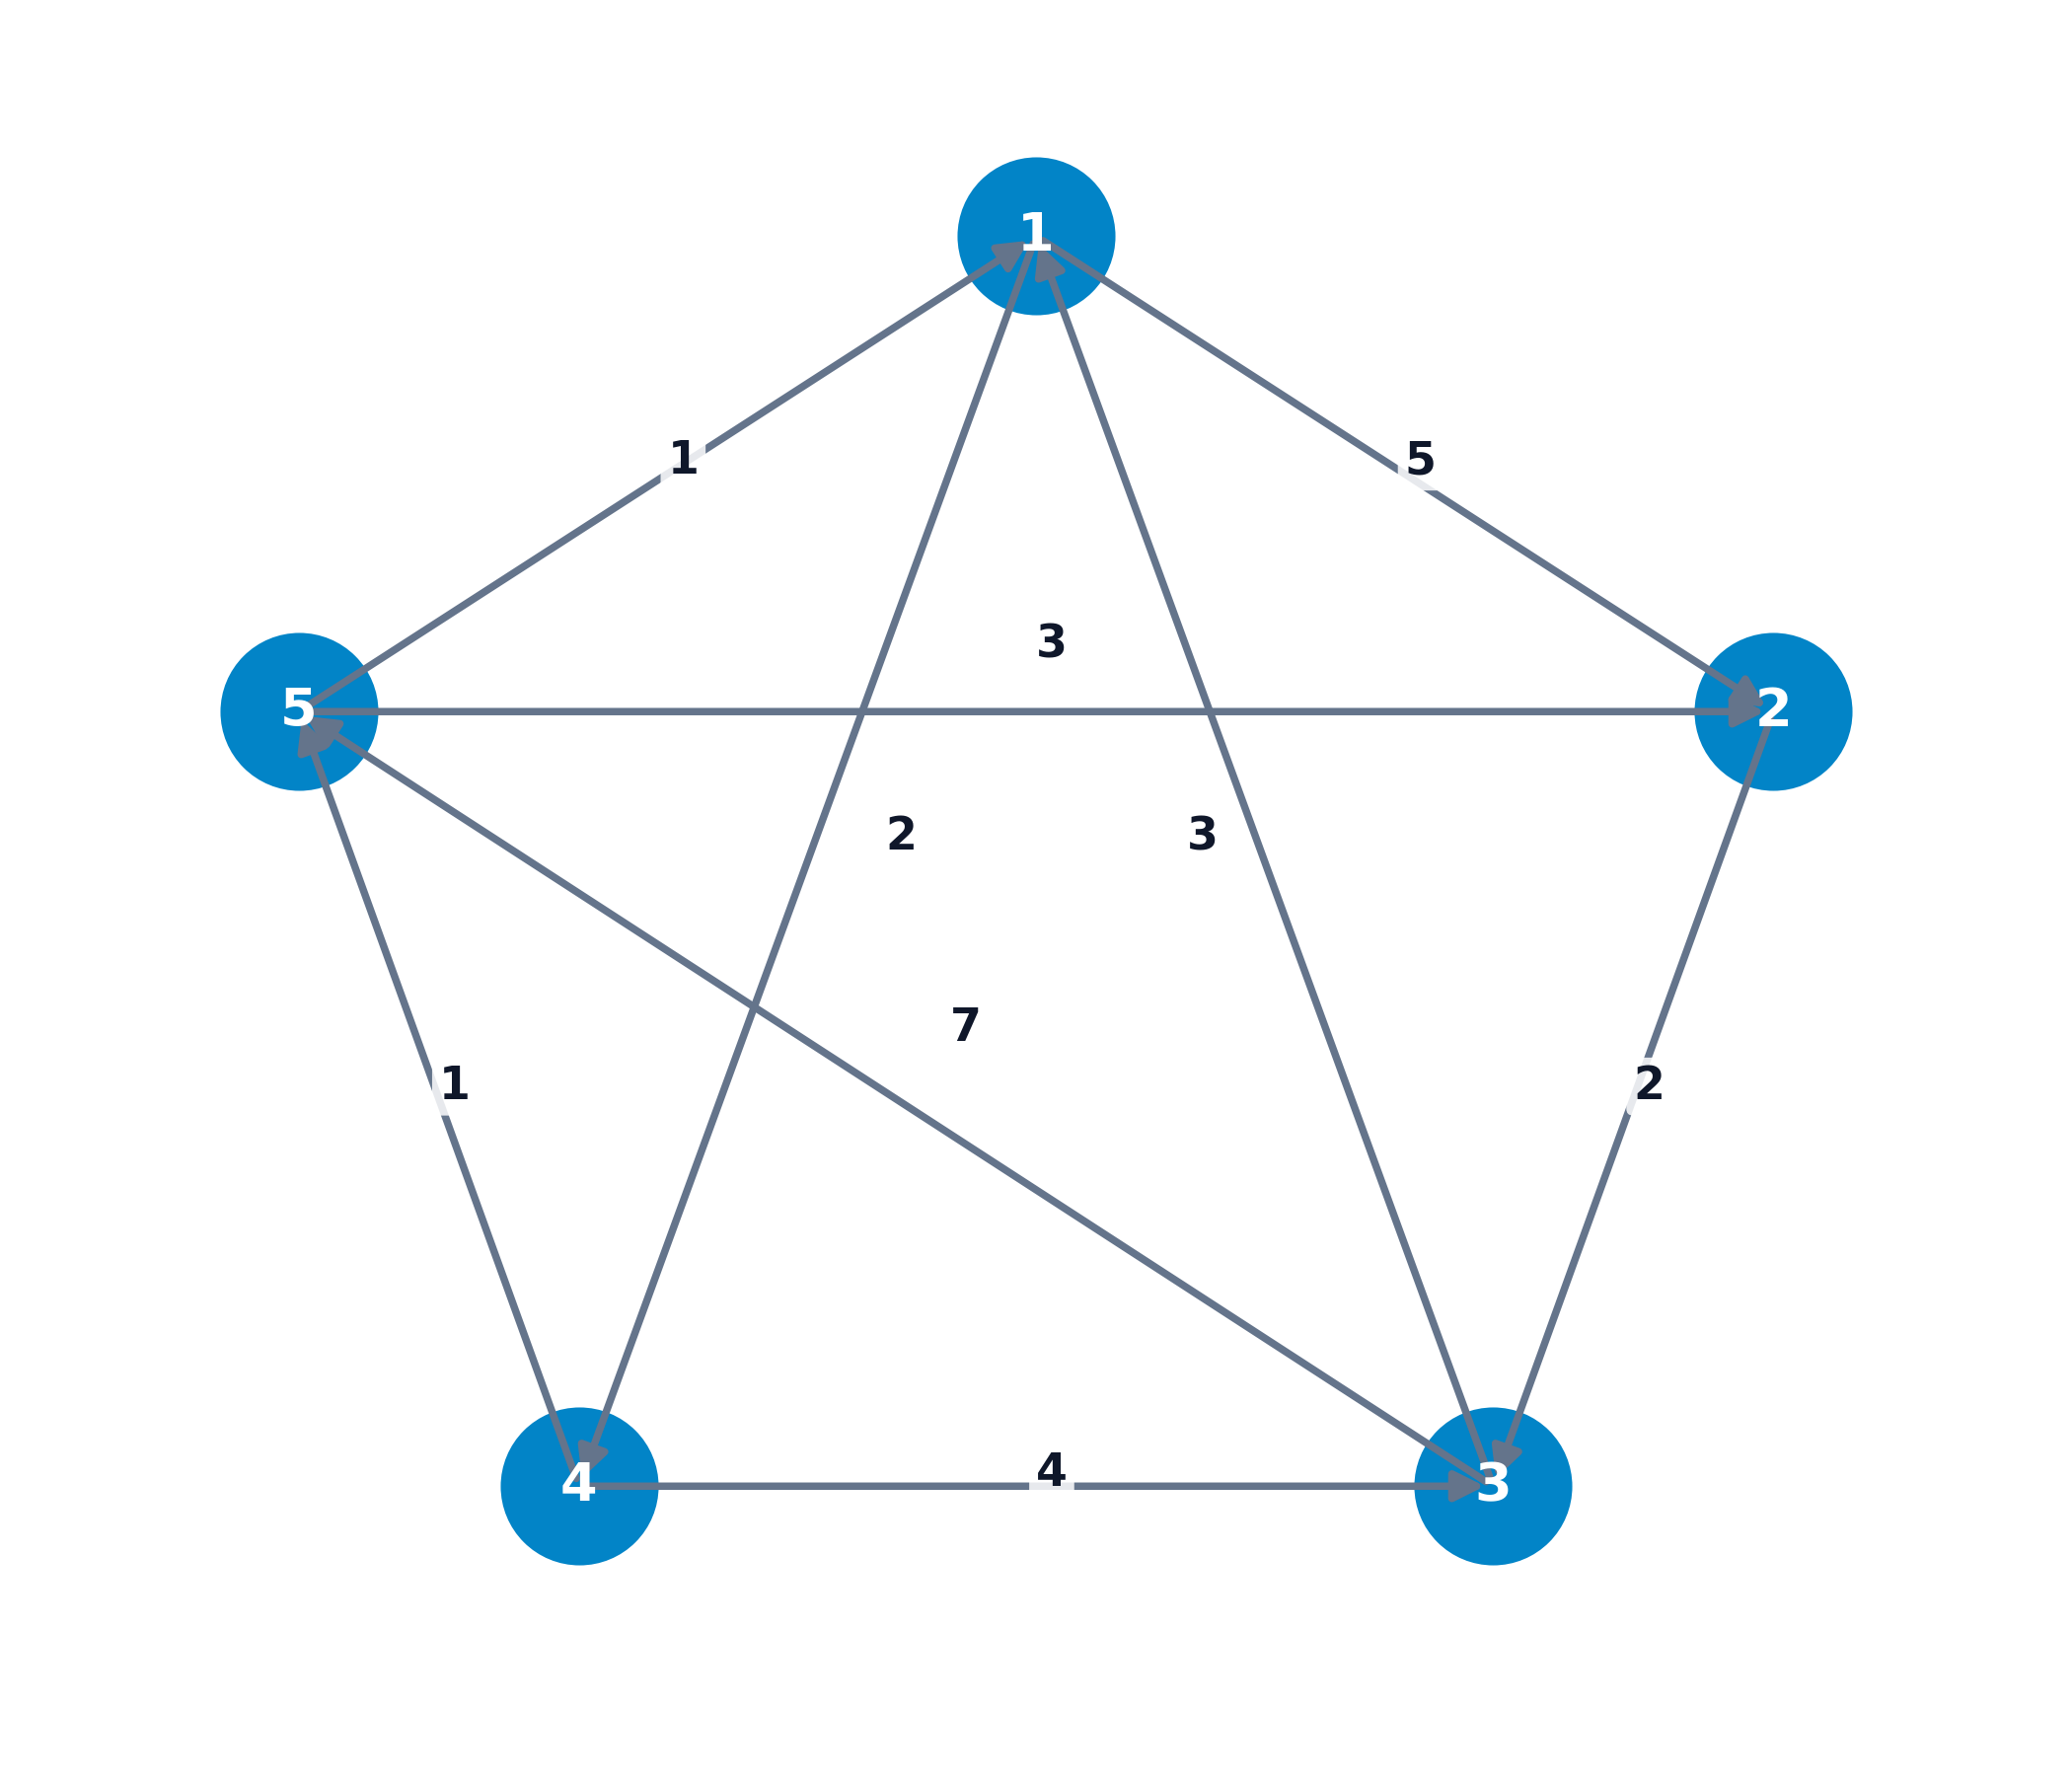
\includegraphics[width=0.95\linewidth,height=\textheight,keepaspectratio]{../images/floyd_warshall_ejemplo_5nodos.png}
\end{center}
\end{column}

\begin{column}{0.5\linewidth}
\begin{itemize}
\item
  \textbf{Digrafo de 5 nodos}: Pivotes secuenciales
  \(k = 1, 2, 3, 4, 5\).
\item
  \textbf{Objetivo}: Obtener la matriz de distancias absolutas
  \(D^{(5)}\) y reconstruir rutas óptimas.
\end{itemize}
\end{column}
\end{columns}
\end{frame}

\begin{frame}{Ejemplo Floyd-Warshall: Matriz Inicial D\^{}(0)}
\phantomsection\label{ejemplo-floyd-warshall-matriz-inicial-d0}
\begin{columns}[T]
\begin{column}{0.42\linewidth}
\begin{center}
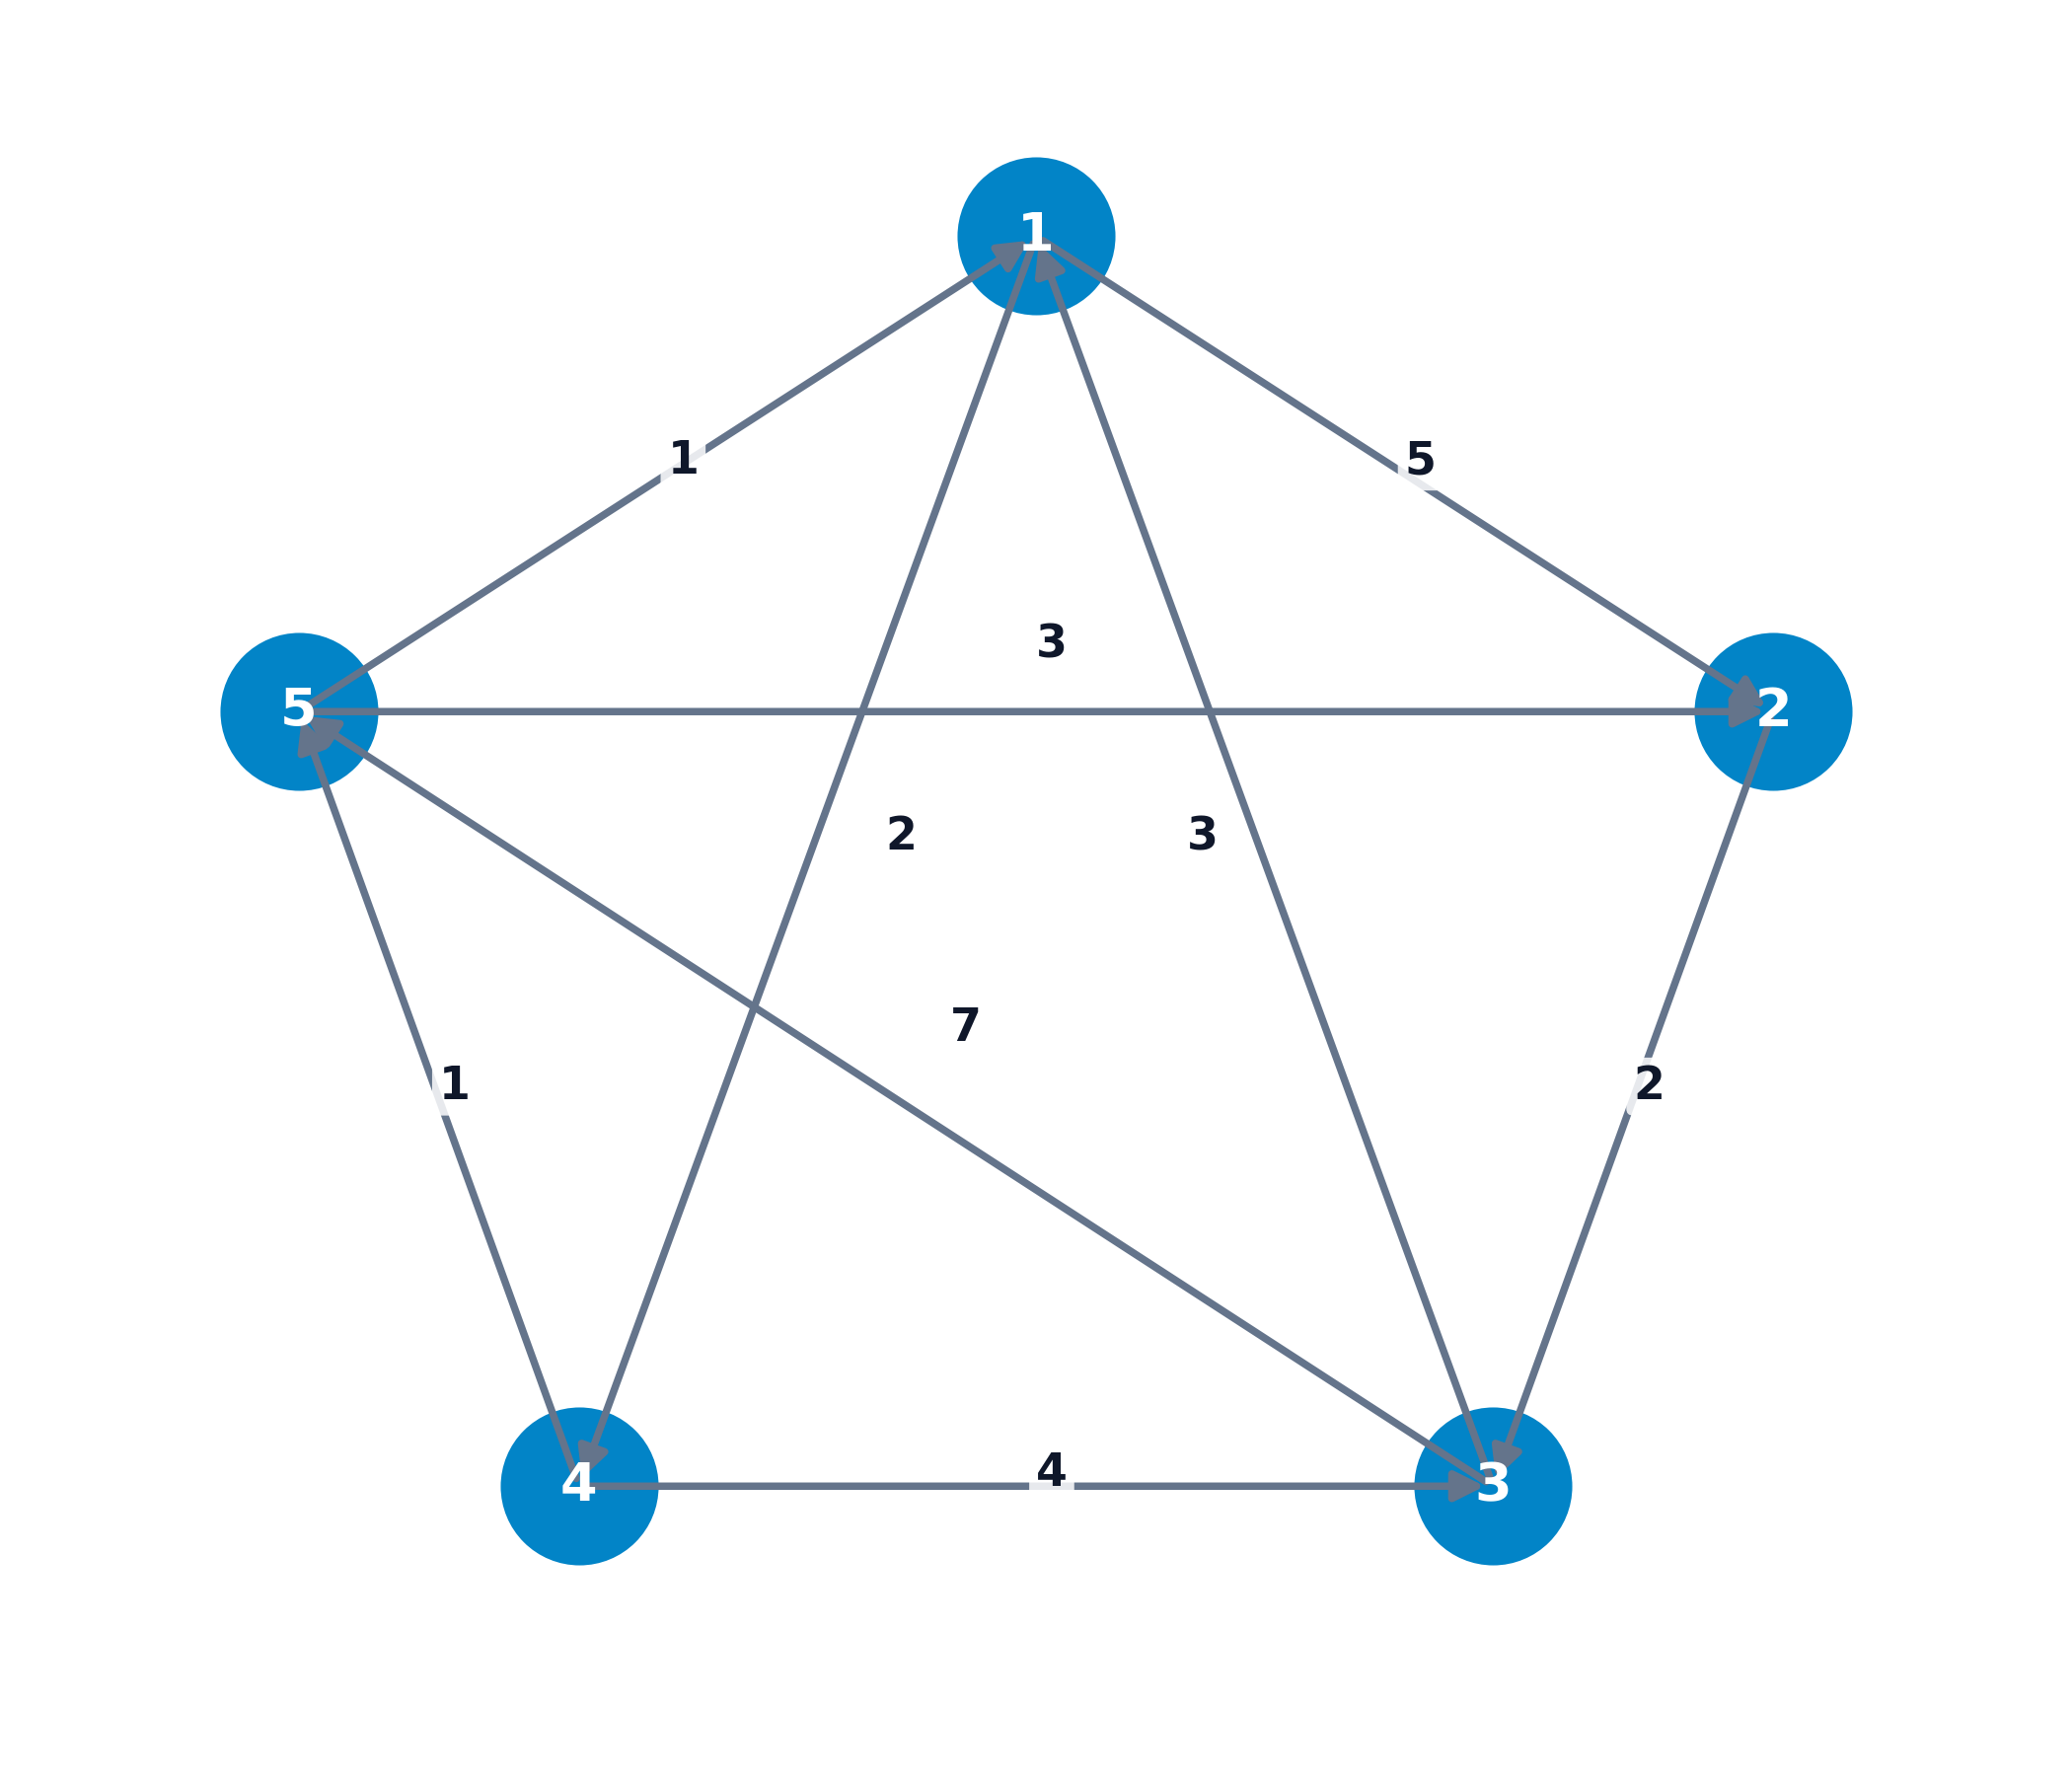
\includegraphics[width=0.95\linewidth,height=\textheight,keepaspectratio]{../images/floyd_warshall_ejemplo_5nodos.png}
\end{center}
\end{column}

\begin{column}{0.58\linewidth}
\begin{itemize}
\item
  \textbf{Matriz Inicial de Distancias Directas \(D^{(0)}\)}: \[ \small
  D^{(0)} = \begin{pmatrix}
  0 & 5 & \infty & 2 & \infty \\
  \infty & 0 & 2 & \infty & \infty \\
  3 & \infty & 0 & \infty & 7 \\
  \infty & \infty & 4 & 0 & 1 \\
  1 & 3 & \infty & \infty & 0
  \end{pmatrix}
  \]
\item
  Contiene las distancias directas entre todo par de vértices
  \(i, j \in V\) antes de aplicar ningún pivote intermedio.
\end{itemize}
\end{column}
\end{columns}
\end{frame}

\begin{frame}{Ejemplo Floyd-Warshall: Iteración k=1 (Pivote nodo 1)}
\phantomsection\label{ejemplo-floyd-warshall-iteraciuxf3n-k1-pivote-nodo-1}
\begin{columns}[T]
\begin{column}{0.48\linewidth}
\begin{itemize}
\tightlist
\item
  \textbf{Evaluación del pivote intermedio \(k=1\)}:

  \begin{itemize}
  \tightlist
  \item
    \textbf{Fila 1}: \((0, 5, \infty, 2, \infty)\)
  \item
    \textbf{Columna 1}: \((0, \infty, 3, \infty, 1)^T\)
  \end{itemize}
\item
  \textbf{Relajaciones de etiquetas}:

  \begin{itemize}
  \tightlist
  \item
    \(d_{32}^{(1)} = \min \{\infty, 3 + 5\} = \mathbf{8}\)
  \item
    \(d_{34}^{(1)} = \min \{\infty, 3 + 2\} = \mathbf{5}\)
  \item
    \(d_{54}^{(1)} = \min \{\infty, 1 + 2\} = \mathbf{3}\)
  \end{itemize}
\end{itemize}
\end{column}

\begin{column}{0.52\linewidth}
\begin{itemize}
\tightlist
\item
  \textbf{Matriz Resultante \(D^{(1)}\)}: \[ \small
  D^{(1)} = \begin{pmatrix}
  0 & 5 & \infty & 2 & \infty \\
  \infty & 0 & 2 & \infty & \infty \\
  3 & \mathbf{8} & 0 & \mathbf{5} & 7 \\
  \infty & \infty & 4 & 0 & 1 \\
  1 & 3 & \infty & \mathbf{3} & 0
  \end{pmatrix}
  \]
\end{itemize}
\end{column}
\end{columns}
\end{frame}

\begin{frame}{Ejemplo Floyd-Warshall: Iteración k=2 (Pivote nodo 2)}
\phantomsection\label{ejemplo-floyd-warshall-iteraciuxf3n-k2-pivote-nodo-2}
\begin{columns}[T]
\begin{column}{0.48\linewidth}
\begin{itemize}
\tightlist
\item
  \textbf{Evaluación del pivote intermedio \(k=2\)}:

  \begin{itemize}
  \tightlist
  \item
    \textbf{Fila 2}: \((\infty, 0, 2, \infty, \infty)\)
  \item
    \textbf{Columna 2}: \((5, 0, 8, \infty, 3)^T\)
  \end{itemize}
\item
  \textbf{Relajaciones de etiquetas}:

  \begin{itemize}
  \tightlist
  \item
    \(d_{13}^{(2)} = \min \{\infty, 5 + 2\} = \mathbf{7}\)
  \item
    \(d_{53}^{(2)} = \min \{\infty, 3 + 2\} = \mathbf{5}\)
  \end{itemize}
\end{itemize}
\end{column}

\begin{column}{0.52\linewidth}
\begin{itemize}
\tightlist
\item
  \textbf{Matriz Resultante \(D^{(2)}\)}: \[ \small
  D^{(2)} = \begin{pmatrix}
  0 & 5 & \mathbf{7} & 2 & \infty \\
  \infty & 0 & 2 & \infty & \infty \\
  3 & 8 & 0 & 5 & 7 \\
  \infty & \infty & 4 & 0 & 1 \\
  1 & 3 & \mathbf{5} & 3 & 0
  \end{pmatrix}
  \]
\end{itemize}
\end{column}
\end{columns}
\end{frame}

\begin{frame}{Ejemplo Floyd-Warshall: Iteración k=3 (Pivote nodo 3)}
\phantomsection\label{ejemplo-floyd-warshall-iteraciuxf3n-k3-pivote-nodo-3}
\begin{columns}[T]
\begin{column}{0.48\linewidth}
\begin{itemize}
\tightlist
\item
  \textbf{Evaluación del pivote intermedio \(k=3\)}:

  \begin{itemize}
  \tightlist
  \item
    \textbf{Fila 3}: \((3, 8, 0, 5, 7)\)
  \item
    \textbf{Columna 3}: \((7, 2, 0, 4, 5)^T\)
  \end{itemize}
\item
  \textbf{Relajaciones de etiquetas}:

  \begin{itemize}
  \tightlist
  \item
    \(d_{15}^{(3)} = \min \{\infty, 7 + 7\} = \mathbf{14}\)
  \item
    \(d_{21}^{(3)} = \min \{\infty, 2 + 3\} = \mathbf{5}\)
  \item
    \(d_{24}^{(3)} = \min \{\infty, 2 + 5\} = \mathbf{7}\)
  \item
    \(d_{25}^{(3)} = \min \{\infty, 2 + 7\} = \mathbf{9}\)
  \item
    \(d_{41}^{(3)} = \min \{\infty, 4 + 3\} = \mathbf{7}\)
  \item
    \(d_{42}^{(3)} = \min \{\infty, 4 + 8\} = \mathbf{12}\)
  \end{itemize}
\end{itemize}
\end{column}

\begin{column}{0.52\linewidth}
\begin{itemize}
\tightlist
\item
  \textbf{Matriz Resultante \(D^{(3)}\)}: \[ \small
  D^{(3)} = \begin{pmatrix}
  0 & 5 & 7 & 2 & \mathbf{14} \\
  \mathbf{5} & 0 & 2 & \mathbf{7} & \mathbf{9} \\
  3 & 8 & 0 & 5 & 7 \\
  \mathbf{7} & \mathbf{12} & 4 & 0 & 1 \\
  1 & 3 & 5 & 3 & 0
  \end{pmatrix}
  \]
\end{itemize}
\end{column}
\end{columns}
\end{frame}

\begin{frame}{Ejemplo Floyd-Warshall: Iteración k=4 (Pivote nodo 4)}
\phantomsection\label{ejemplo-floyd-warshall-iteraciuxf3n-k4-pivote-nodo-4}
\begin{columns}[T]
\begin{column}{0.48\linewidth}
\begin{itemize}
\tightlist
\item
  \textbf{Evaluación del pivote intermedio \(k=4\)}:

  \begin{itemize}
  \tightlist
  \item
    \textbf{Fila 4}: \((7, 12, 4, 0, 1)\)
  \item
    \textbf{Columna 4}: \((2, 7, 5, 0, 3)^T\)
  \end{itemize}
\item
  \textbf{Relajaciones de etiquetas}:

  \begin{itemize}
  \tightlist
  \item
    \(d_{13}^{(4)} = \min \{7, 2 + 4\} = \mathbf{6}\)
  \item
    \(d_{15}^{(4)} = \min \{14, 2 + 1\} = \mathbf{3}\)
  \item
    \(d_{25}^{(4)} = \min \{9, 7 + 1\} = \mathbf{8}\)
  \item
    \(d_{35}^{(4)} = \min \{7, 5 + 1\} = \mathbf{6}\)
  \end{itemize}
\end{itemize}
\end{column}

\begin{column}{0.52\linewidth}
\begin{itemize}
\tightlist
\item
  \textbf{Matriz Resultante \(D^{(4)}\)}: \[ \small
  D^{(4)} = \begin{pmatrix}
  0 & 5 & \mathbf{6} & 2 & \mathbf{3} \\
  5 & 0 & 2 & 7 & \mathbf{8} \\
  3 & 8 & 0 & 5 & \mathbf{6} \\
  7 & 12 & 4 & 0 & 1 \\
  1 & 3 & 5 & 3 & 0
  \end{pmatrix}
  \]
\end{itemize}
\end{column}
\end{columns}
\end{frame}

\begin{frame}{Ejemplo Floyd-Warshall: Iteración k=5 (Matriz Final
D\^{}(5))}
\phantomsection\label{ejemplo-floyd-warshall-iteraciuxf3n-k5-matriz-final-d5}
\begin{columns}[T]
\begin{column}{0.48\linewidth}
\begin{itemize}
\tightlist
\item
  \textbf{Evaluación del pivote intermedio \(k=5\)}:

  \begin{itemize}
  \tightlist
  \item
    \textbf{Fila 5}: \((1, 3, 5, 3, 0)\)
  \item
    \textbf{Columna 5}: \((3, 8, 6, 1, 0)^T\)
  \end{itemize}
\item
  \textbf{Relajaciones finales}:

  \begin{itemize}
  \tightlist
  \item
    \(d_{41}^{(5)} = \min \{7, 1 + 1\} = \mathbf{2}\)
  \item
    \(d_{42}^{(5)} = \min \{12, 1 + 3\} = \mathbf{4}\)
  \end{itemize}
\item
  \textbf{Conclusión}: \(D^{(5)}\) determina la distancia geodésica
  exacta entre todo par de vértices.
\end{itemize}
\end{column}

\begin{column}{0.52\linewidth}
\begin{itemize}
\tightlist
\item
  \textbf{Matriz Final \(D^{(5)}\)}: \[ \small
  D^{(5)} = \begin{pmatrix}
  0 & 5 & 6 & 2 & 3 \\
  5 & 0 & 2 & 7 & 8 \\
  3 & 8 & 0 & 5 & 6 \\
  \mathbf{2} & \mathbf{4} & 4 & 0 & 1 \\
  1 & 3 & 5 & 3 & 0
  \end{pmatrix}
  \]
\end{itemize}
\end{column}
\end{columns}
\end{frame}

\begin{frame}{Ejemplo Floyd-Warshall: Reconstrucción de la ruta óptima
(4, 2)}
\phantomsection\label{ejemplo-floyd-warshall-reconstrucciuxf3n-de-la-ruta-uxf3ptima-4-2}
\begin{itemize}
\item
  \textbf{Matriz de predecesores final \(P^{(5)}\)}:
  \[\text{Para el par }(4, 2): \quad P_{42} = 5\]
\item
  \textbf{Traza de reconstrucción}:

  \begin{enumerate}
  \tightlist
  \item
    De 4 a 2: El primer paso intermedio pasa por el nodo 5 \(\implies\)
    segmento \(4 \to 5\).
  \item
    De 5 a 2: Inspeccionar \(P_{52} = 2 \implies\) segmento directo
    \(5 \to 2\).
  \end{enumerate}
\item
  \textbf{Ruta elemental óptima}: \[4 \to 5 \to 2\]

  \begin{itemize}
  \tightlist
  \item
    Coste acumulado: \(d_{45} + d_{52} = 1 + 3 = \mathbf{4}\) (coincide
    con \(d_{42}^{(5)} = 4\)).
  \end{itemize}
\end{itemize}
\end{frame}

\begin{frame}{Ejemplo Floyd-Warshall: Traza animada interactiva}
\phantomsection\label{ejemplo-floyd-warshall-traza-animada-interactiva}
\end{frame}




\end{document}
